% !TeX spellcheck = en-US
% !TeX encoding = utf8
% !TeX program = pdflatex
% !BIB program = biber
% -*- coding:utf-8 mod:LaTeX -*-


% vv  scroll down to line 200 for content  vv


\let\ifdeutsch\iffalse
\let\ifenglish\iftrue


% EN: This file is loaded before the \documentclass command in the main document

% EN: The following package allows \\ at the title page
%     For more information see https://github.com/latextemplates/scientific-thesis-cover/issues/4
\RequirePackage{kvoptions-patch}

\ifenglish
  \PassOptionsToClass{numbers=noenddot}{scrbook}
\else
  %()Aus scrguide.pdf - der Dokumentation von KOMA-Script)
  %Nach DUDEN steht in Gliederungen, in denen ausschließlich arabische Ziffern für die Nummerierung
  %verwendet werden, am Ende der Gliederungsnummern kein abschließender Punkt
  %(siehe [DUD96, R3]). Wird hingegen innerhalb der Gliederung auch mit römischen Zahlen
  %oder Groß- oder Kleinbuchstaben gearbeitet, so steht am Ende aller Gliederungsnummern ein
  %abschließender Punkt (siehe [DUD96, R4])
  \PassOptionsToClass{numbers=autoendperiod}{scrbook}
\fi

% Warns about outdated packages and missing caption declarations
% See https://www.ctan.org/pkg/nag
\RequirePackage[l2tabu, orthodox]{nag}

%DE: Neue deutsche Trennmuster
%    Siehe http://www.ctan.org/pkg/dehyph-exptl und http://projekte.dante.de/Trennmuster/WebHome
%    Nur für pdflatex, nicht für lualatex
\RequirePackage{ifluatex}
\ifluatex
  % do not load anything
\else
  \ifdeutsch
    \RequirePackage[ngerman=ngerman-x-latest]{hyphsubst}
  \fi
\fi

\documentclass[
  %
  %ngerman, %%% Add if you write in German.
  %
  % fontsize=11pt is the standard
  a4paper,  % Standard format - only KOMAScript uses paper=a4 - https://tex.stackexchange.com/a/61044/9075
  twoside,  % we are optimizing for both screen and two-side printing. So the page numbers will jump, but the content is configured to stay in the middle (by using the geometry package)
  bibliography=totoc,
  %               idxtotoc,   %Index ins Inhaltsverzeichnis
  %               liststotoc, %List of X ins Inhaltsverzeichnis, mit liststotocnumbered werden die Abbildungsverzeichnisse nummeriert
  headsepline,
  cleardoublepage=empty,
  parskip=half,
  %               draft    % um zu sehen, wo noch nachgebessert werden muss - wichtig, da Bindungskorrektur mit drin
  draft=false
]{scrbook}
% !TeX encoding = utf8
% -*- coding:utf-8 mod:LaTeX -*-

% EN: This file includes basic packages and sets options. The order of package
%     loading is important

% DE: In dieser Datei werden zuerst die benoetigten Pakete eingebunden und
%     danach diverse Optionen gesetzt. Achtung Reihenfolge ist entscheidend!


% EN: Styleguide:
% - English comments are prefixed with "EN", German comments are prefixed with "DE"
% - Prefixed headings define the language for the subsequent paragraphs
% - It is tried to organize packages in blocks. Bocks are separated by two empty lines.

% DE: Styleguide:
%
% Ein sehr kleiner Styleguide. Packages werden in Blöcken organisiert.
% Zwischen zwei Blöcken sind 2 Leerzeilen!


% EN: Enable copy and paste of text from the PDF
%     Only required for pdflatex. It "just works" in the case of lualatex.
%     mmap enables mathematical symbols, but does not work with the newtx font set
%     See: https://tex.stackexchange.com/a/64457/9075
%     Other solutions outlined at http://goemonx.blogspot.de/2012/01/pdflatex-ligaturen-und-copynpaste.html and http://tex.stackexchange.com/questions/4397/make-ligatures-in-linux-libertine-copyable-and-searchable
%     Trouble shooting outlined at https://tex.stackexchange.com/a/100618/9075

\ifluatex
\else
  \usepackage{cmap}
\fi


% EN: File encoding
% DE: Codierung
%     Wir sind im 21 Jahrhundert, utf-8 löst so viele Probleme.
%
% Mit UTF-8 funktionieren folgende Pakete nicht mehr. Bitte beachten!
%   * fancyvrb mit §
%   * easylist -> http://www.ctan.org/tex-archive/macros/latex/contrib/easylist/
\ifluatex
  % EN: See https://tex.stackexchange.com/a/158517/9075
  %     Not required, because of usage of fontspec package
  %\usepackage[utf8]{luainputenc}
\else
  \usepackage[utf8]{inputenc}
\fi


% DE: Parallelbetrieb tex4ht und pdflatex

\makeatletter
\@ifpackageloaded{tex4ht}{
  \def\iftex4ht{\iftrue}
}{
  \def\iftex4ht{\iffalse}
}
\makeatother


% EN: Mathematics
% DE: Mathematik
%
% DE: Viele Mathematik-Sachen. Siehe https://texdoc.net/pkg/amsmath
%
% EN: Options must be passed this way, otherwise it does not work with glossaries
% DE: fleqn (=Gleichungen linksbündig platzieren) funktioniert nicht direkt. Es muss noch ein Patch gemacht werden:
\PassOptionsToPackage{fleqn,leqno}{amsmath}
%
% DE: amsmath Muss nicht mehr geladen werden, da es von newtxmath automatisch geladen wird
% \usepackage{amsmath}


%% EN: Fonts
%% DE: Schriften
%%
%% !!! If you change the font, be sure that words such as "workflow" can
%% !!! still be copied from the PDF. If this is not the case, you have
%% !!! to use glyphtounicode. See comment at cmap package


% EN: Times Roman for all text
\ifluatex
  % source: Second proposed fix from the following answer: https://tex.stackexchange.com/a/394137
  \usepackage[no-math]{fontspec}
  \setmainfont{TeXGyreTermes-Regular}[
       BoldFont       = TeXGyreTermes-Bold ,
       ItalicFont     = TeXGyreTermes-Italic ,
       BoldItalicFont = TeXGyreTermes-BoldItalic,
       NFSSFamily     = ntxtlf]
  \setsansfont{TeX Gyre Heros Regular}[
       Scale=.9,
       BoldFont       = TeX Gyre Heros Bold,
       ItalicFont     = TeX Gyre Heros Italic,
       BoldItalicFont = TeX Gyre Heros BoldItalic]
  \setmonofont[StylisticSet={1,3},Scale=.9]{inconsolata}
  \RequirePackage{newtxmath}
\else
  \RequirePackage{newtxtext}
  \RequirePackage{newtxmath}
  % EN: looks good with times, but no equivalent for lualatex found,
  %     therefore replaced with inconsolata
  %\RequirePackage[zerostyle=b,scaled=.9]{newtxtt}
  \RequirePackage[varl,scaled=.9]{inconsolata}
\fi

% EN: Fallback font - if the subsequent font packages do not define a font (e.g., monospaced)
%     This is the modern package for "Computer Modern".
%     In case this gets activated, one has to switch from cmap package to glyphtounicode (in the case of pdflatex)
% DE: Fallback-Schriftart
%\usepackage[%
%    rm={oldstyle=false,proportional=true},%
%    sf={oldstyle=false,proportional=true},%
%    tt={oldstyle=false,proportional=true,variable=true},%
%    qt=false%
%]{cfr-lm}

% EN: Headings are typset in Helvetica (which is similar to Arial)
% DE: Schriftart fuer die Ueberschriften - ueberschreibt lmodern
%\usepackage[scaled=.95]{helvet}

% DE: Für Schreibschrift würde tun, muss aber nicht
%\usepackage{mathrsfs} %  \mathscr{ABC}

% EN: Font for the main text
% DE: Schriftart fuer den Fliesstext - ueberschreibt lmodern
%     Linux Libertine, siehe http://www.linuxlibertine.org/
%     Packageparamter [osf] = Minuskel-Ziffern
%     rm = libertine im Brottext, Linux Biolinum NICHT als serifenlose Schrift, sondern helvet (von oben) beibehalten
%\usepackage[rm]{libertine}

% EN: Alternative Font: Palantino. It is recommeded by Prof. Ludewig for German texts
% DE: Alternative Schriftart: Palantino, Packageparamter [osf] = Minuskel-Ziffern
%     Bitte nur in deutschen Texten
%\usepackage{mathpazo} %ftp://ftp.dante.de/tex-archive/fonts/mathpazo/ - Tipp aus DE-TEX-FAQ 8.2.1

% DE: Schriftart fuer Programmcode - ueberschreibt lmodern
%     Falls auskommentiert, wird die Standardschriftart lmodern genommen
%     Fuer schreibmaschinenartige Schluesselwoerter in den Listings - geht bei alten Installationen nicht, da einige Fontshapes (<>=) fehlen
%\usepackage[scaled=.92]{luximono}
%\usepackage{courier}
% DE: BeraMono als Typewriter-Schrift, Tipp von http://tex.stackexchange.com/a/71346/9075
%\usepackage[scaled=0.83]{beramono}

% EN: backticks (`) are rendered as such in verbatim environments.
%     See following links for details:
%     - https://tex.stackexchange.com/a/341057/9075
%     - https://tex.stackexchange.com/a/47451/9075
%     - https://tex.stackexchange.com/a/166791/9075
\usepackage{upquote}

% DE: Symbole
%
%\usepackage[geometry]{ifsym} % \BigSquare
%\usepackage{mathabx}
%\usepackage{stmaryrd} %fuer \ovee, \owedge, \otimes
%\usepackage{marvosym} %fuer \Writinghand %patched to not redefine \Rightarrow
%\usepackage{mathrsfs} %mittels \mathscr{} schoenen geschwungenen Buchstaben erzeugen
%\usepackage{calrsfs} %\mathcal{} ein bisserl dickeren buchstaben erzeugen - sieht net so gut aus.
%durch mathpazo ist das schon definiert

%
%\usepackage{amssymb}

% EN: For \texttrademark{}
\usepackage{textcomp}

% EN: name-clashes von marvosym und mathabx vermeiden:
\def\delsym#1{%
  %  \expandafter\let\expandafter\origsym\expandafter=\csname#1\endcsname
  %  \expandafter\let\csname orig#1\endcsname=\origsym
  \expandafter\let\csname#1\endcsname=\relax
}

%\usepackage{pifont}
%\usepackage{bbding}
%\delsym{Asterisk}
%\delsym{Sun}\delsym{Mercury}\delsym{Venus}\delsym{Earth}\delsym{Mars}
%\delsym{Jupiter}\delsym{Saturn}\delsym{Uranus}\delsym{Neptune}
%\delsym{Pluto}\delsym{Aries}\delsym{Taurus}\delsym{Gemini}
%\delsym{Rightarrow}
%\usepackage{mathabx} - Ueberschreibt leider zu viel - und die \le-Zeichen usw. sehen nicht gut aus!


% EN: Modern font encoding
%     Has to be loaded AFTER any font packages. See https://tex.stackexchange.com/a/2869/9075.
\ifluatex
\else
  \usepackage[T1]{fontenc}
\fi
%


% EN: Character protrusion and font expansion. See http://www.ctan.org/tex-archive/macros/latex/contrib/microtype/
% DE: Optischer Randausgleich und Grauwertkorrektur

\usepackage[
  babel=true, % EN: Enable language-specific kerning. Take language-settings from the languge of the current document (see Section 6 of microtype.pdf)
  expansion=alltext,
  protrusion=alltext-nott, % EN: Ensure that at listings, there is no change at the margin of the listing
  final % EN: Always enable microtype, even if in draft mode. This helps finding bad boxes quickly.
        %     In the standard configuration, this template is always in the final mode, so this option only makes a difference if "pros" use the draft mode
]{microtype}


% EN: \texttt{test -- test} keeps the "--" as "--" (and does not convert it to an en dash)
\DisableLigatures{encoding = T1, family = tt* }

% DE: fuer microtype
% DE: tracking=true muss als Parameter des microtype-packages mitgegeben werden
% DE: Deaktiviert, da dies bei Algorithmen seltsam aussieht

%\DeclareMicrotypeSet*[tracking]{my}{ font = */*/*/sc/* }%
%\SetTracking{ encoding = *, shape = sc }{ 45 }
% DE: Hier wird festgelegt,
%     dass alle Passagen in Kapitälchen automatisch leicht
%     gesperrt werden.
%     Quelle: http://homepage.ruhr-uni-bochum.de/Georg.Verweyen/pakete.html
%    Deaktiviert, da sonst "BPEL", "BPMN" usw. wirklich komisch aussehen.
%     Macht wohl nur bei geisteswissenschaftlichen Arbeiten Sinn.


% EN: amsmath teaks


% EN: Fixes bugs in AMS math
%     Corrently conflicts with unicode-math
% \usepackage{mathtools}

%\numberwithin{equation}{section}
%\renewcommand{\theequation}{\thesection.\Roman{equation}}

% EN: work-around ams-math problem with align and 9 -> 10. Does not work with glossaries, No visual changes.
%\addtolength\mathindent{1em}


% EN: For theorems, replacement for amsthm
\usepackage[amsmath,hyperref]{ntheorem}
\theorempreskipamount 2ex plus1ex minus0.5ex
\theorempostskipamount 2ex plus1ex minus0.5ex
\theoremstyle{break}
\newtheorem{definition}{Definition}[section]


% CTAN: https://ctan.org/pkg/lccaps
% Doc: http://texdoc.net/pkg/lccaps
%
% Required for DE/EN \initialism
\usepackage{lccaps}


% EN: Defintion of colors. Argument "hyperref" is not used as we do not want to change border colors of links: Links are not colored anymore.
% DE: Farbdefinitionen
\usepackage[dvipsnames]{xcolor}


% EN: Required for custom acronyms/glossaries style.
%     Left aligned Columns in tables with fixed width.
%     See http://tex.stackexchange.com/questions/91566/syntax-similar-to-centering-for-right-and-left
\usepackage{ragged2e}


% DE: Wichtig, ansonsten erscheint "No room for a new \write"
\usepackage{scrwfile}


% EN: Support for language-specific hyphenation
% DE: Neue deutsche Rechtschreibung und Literatur statt "Literature"
%     Die folgende Einstellung ist der Nachfolger von ngerman.sty
\ifdeutsch
  % DE: letzte Sprache ist default, Einbindung von "american" ermöglicht \begin{otherlanguage}{amercian}...\end{otherlanguage} oder \foreignlanguage{american}{Text in American}
  %     Siehe auch http://tex.stackexchange.com/a/50638/9075
  \usepackage[american,main=ngerman]{babel}
  % Ein "abstract" ist eine "Kurzfassung", keine "Zusammenfassung"
  \addto\captionsngerman{%
    \renewcommand\abstractname{Kurzfassung}%
  }
  \ifluatex
    % EN: conditionally disable ligatures. See https://github.com/latextemplates/scientific-thesis-template/issues/54
    %     for a discussion
    \usepackage[ngerman]{selnolig}
  \fi
\else
  % EN: Set English as language and allow to write hyphenated"=words
  %     `american`, `english` and `USenglish` are synonyms for babel package (according to https://tex.stackexchange.com/questions/12775/babel-english-american-usenglish).
  %      "english" has to go last to set it as default language
  \usepackage[english]{babel}
  % EN: Hint by http://tex.stackexchange.com/a/321066/9075 -> enable "= as dashes
  \addto\extrasenglish{\languageshorthands{ngerman}\useshorthands{"}}
  \ifluatex
    % EN: conditionally disable ligatures. See https://github.com/latextemplates/scientific-thesis-template/issues/54
    %     for a discussion
    \usepackage[english]{selnolig}
  \fi
\fi
%


% EN: For easy quotations: \enquote{text}
%     This package is very smart when nesting is applied, otherwise textcmds (see below) provides a shorter command
%     Note that this package results in a warning when it is loaded before minted (actually fvextra).
% DE: Anführungszeichen
%     Zitate in \enquote{...} setzen, dann werden automatisch die richtigen Anführungszeichen verwendet.
%     Dieses package erzeugt eine Warnung, wenn es vor minted (genauer fvextra) geladen wird.
\usepackage{csquotes}


% EN: For even easier quotations: \qq{text}.
%     Is not smart in the case of nesting, but good enough for the most cases
\usepackage{textcmds}
\ifdeutsch
  % EN: German quotes are different. So do not use the English quotes, but the ones provided by the csquotes package.
  \renewcommand{\qq}[1]{\enquote{#1}}
\fi


% EN: extended enumarations
% DE: erweitertes Enumerate
\usepackage{paralist}


% DE: Gestaltung der Kopf- und Fußteilen

\usepackage[automark]{scrlayer-scrpage}

\automark[section]{chapter}
\setkomafont{pageheadfoot}{\normalfont\sffamily}
\setkomafont{pagenumber}{\normalfont\sffamily}

% DE: funktioniert nicht: Alle Linien sind hier weg
%\setheadsepline[.4pt]{.4pt}


% DE: Intelligentes Leerzeichen um hinter Abkürzungen die richtigen Abstände zu erhalten, auch leere.
%     Siehe commands.tex \gq{}
\usepackage{xspace}
% DE: Macht \xspace und \enquote kompatibel
\makeatletter
\xspaceaddexceptions{\grqq \grq \csq@qclose@i \} }
\makeatother


\newcommand{\eg}{e.\,g.,\ }
\newcommand{\ie}{i.\,e.,\ }


% EN: introduce \powerset - hint by http://matheplanet.com/matheplanet/nuke/html/viewtopic.php?topic=136492&post_id=997377
\DeclareFontFamily{U}{MnSymbolC}{}
\DeclareSymbolFont{MnSyC}{U}{MnSymbolC}{m}{n}
\DeclareFontShape{U}{MnSymbolC}{m}{n}{
  <-6>    MnSymbolC5
  <6-7>   MnSymbolC6
  <7-8>   MnSymbolC7
  <8-9>   MnSymbolC8
  <9-10>  MnSymbolC9
  <10-12> MnSymbolC10
  <12->   MnSymbolC12%
}{}
\DeclareMathSymbol{\powerset}{\mathord}{MnSyC}{180}


% EN: Package for the appendix
% DE: Anhang
\usepackage{appendix}
%[toc,page,title,header]
%


% EN: Graphics
% DE: Grafikeinbindungen
%
% EN: The parameter "pdftex" is not required
\usepackage{graphicx}
\graphicspath{{\getgraphicspath}}
\newcommand{\getgraphicspath}{graphics/}


% EN: Enables inclusion of SVG graphics - 1:1 approach
%    This is NOT the approach of https://ctan.org/pkg/svg-inkscape,
%     which allows text in SVG to be typeset using LaTeX
%     We just include the SVG as is.
\usepackage{epstopdf}
\epstopdfDeclareGraphicsRule{.svg}{pdf}{.pdf}{%
  inkscape -z -D --file=#1 --export-pdf=\OutputFile
}


% EN: Enables inclusion of SVG graphics - text-rendered-with-LaTeX-approach
%     This is the approach of https://ctan.org/pkg/svg-inkscape,
\newcommand{\executeiffilenewer}[3]{%
  \IfFileExists{#2}
  {
    %\message{file #2 exists}
    \ifnum\pdfstrcmp{\pdffilemoddate{#1}}%
      {\pdffilemoddate{#2}}>0%
      {\immediate\write18{#3}}
    \else
      {%\message{file up to date #2}
      }
    \fi%
  }{
    %\message{file #2 doesn't exist}
    %\message{argument: #3}
    %\immediate\write18{echo "test" > xoutput.txt}
    \immediate\write18{#3}
  }
}
\newcommand{\includesvg}[1]{%
  \executeiffilenewer{#1.svg}{#1.pdf}%
  {
    inkscape -z -D --file=\getgraphicspath#1.svg %
    --export-pdf=\getgraphicspath#1.pdf --export-latex}%
  \input{\getgraphicspath#1.pdf_tex}%
}


% EN: Enable typesetting values with SI units.
%\ifdeutsch
%  \usepackage[mode=text,group-four-digits]{siunitx}
%  \sisetup{locale=DE}
%\else
%  \usepackage[mode=text,group-four-digits,group-separator={,}]{siunitx}
%  \sisetup{locale=US}
%\fi


% EN: Extensions for tables
% DE: Tabellenerweiterungen
\usepackage{array} %increases tex's buffer size and enables ``>'' in tablespecs
\usepackage{longtable}
\usepackage{dcolumn} %Aligning numbers by decimal points in table columns
\ifdeutsch
  \newcolumntype{d}[1]{D{.}{,}{#1}}
\else
  \newcolumntype{d}[1]{D{.}{.}{#1}}
\fi
\setlength{\extrarowheight}{1pt}


% DE: Eine Zelle, die sich über mehrere Zeilen erstreckt.
%     Siehe Beispieltabelle in Kapitel 2
\usepackage{multirow}


% DE: Fuer Tabellen mit Variablen Spaltenbreiten
%\usepackage{tabularx}
%\usepackage{tabulary}


% EN: Links behave as they should. Enables "\url{...}" for URL typesettings.
%     Allow URL breaks also at a hyphen, even though it might be confusing: Is the "-" part of the address or just a hyphen?
%     See https://tex.stackexchange.com/a/3034/9075.
% DE: Links verhalten sich so, wie sie sollen
%     Zeilenumbrüche bei URLs auch bei Bindestrichen erlauben, auch wenn es verwirrend sein könnte: Gehört der Bindestrich zur URL oder ist es ein Trennstrich?
%     Siehe https://tex.stackexchange.com/a/3034/9075.
\usepackage[hyphens]{url}
%
%  EN: When activated, use text font as url font, not the monospaced one.
%      For all options see https://tex.stackexchange.com/a/261435/9075.
% \urlstyle{same}
%
% EN: Hint by http://tex.stackexchange.com/a/10419/9075.
\makeatletter
\g@addto@macro{\UrlBreaks}{\UrlOrds}
\makeatother


% DE: Index über Begriffe, Abkürzungen
%\usepackage{makeidx} makeidx ist out -> http://xindy.sf.net verwenden


% DE: lustiger Hack fuer das Abkuerzungsverzeichnis
%     nach latex durchlauf folgendes ausfuehren
%     makeindex ausarbeitung.nlo -s nomencl.ist -o ausarbeitung.nls
%     danach nochmal latex
%\usepackage{nomencl}
%    \let\abk\nomenclature %Deutsche Ueberschrift setzen
%          \renewcommand{\nomname}{List of Abbreviations}
%        %Punkte zw. Abkuerzung und Erklaerung
%          \setlength{\nomlabelwidth}{.2\hsize}
%          \renewcommand{\nomlabel}[1]{#1 \dotfill}
%        %Zeilenabstaende verkleinern
%          \setlength{\nomitemsep}{-\parsep}
%    \makenomenclature


% EN: Logic for TeX - enables if-then-else in commands
% DE: Logik für TeX
%     FÜr if-then-else @ commands.tex
\usepackage{ifthen}


% EN: Code Listings
% DE: Listings
\usepackage{listings}
\lstset{language=XML,
  showstringspaces=false,
  extendedchars=true,
  basicstyle=\footnotesize\ttfamily,
  commentstyle=\slshape,
  % DE: Original: \rmfamily, damit werden die Strings im Quellcode hervorgehoben. Zusaetzlich evtl.: \scshape oder \rmfamily durch \ttfamily ersetzen. Dann sieht's aus, wie bei fancyvrb
  stringstyle=\ttfamily,
  breaklines=true,
  breakatwhitespace=true,
  % EN: alternative: fixed
  columns=flexible,
  numbers=left,
  numberstyle=\tiny,
  basewidth=.5em,
  xleftmargin=.5cm,
  % aboveskip=0mm, %DE: deaktivieren, falls man lstlistings direkt als floating object benutzt (\begin{lstlisting}[float,...])
  % belowskip=0mm, %DE: deaktivieren, falls man lstlistings direkt als floating object benutzt (\begin{lstlisting}[float,...])
  captionpos=b
}

\ifluatex
\else
  % EN: Enable UTF-8 support - see https://tex.stackexchange.com/q/419327/9075
  \usepackage{listingsutf8}
  \lstset{inputencoding=utf8/latin1}
\fi

\ifdeutsch
  \renewcommand{\lstlistlistingname}{Verzeichnis der Listings}
\fi


% EN: Alternative to listings could be fancyvrb. Can be used together.
% DE: Alternative zu Listings ist fancyvrb. Kann auch beides gleichzeitig benutzt werden.
\usepackage{fancyvrb}
%
% EN: Font size for the normal text
% DE: Groesse fuer den Fliesstext. Falls deaktiviert: \normalsize
%\fvset{fontsize=\small}
%
% DE: Somit kann im Text ganz einfach §verbatim§ text gesetzt werden.
%     Disabled, because UTF-8 does not work any more and lualatex causes issues
%\DefineShortVerb{\§}
%
% EN: Shrink font size of listings
\RecustomVerbatimEnvironment{Verbatim}{Verbatim}{fontsize=\footnotesize}
\RecustomVerbatimCommand{\VerbatimInput}{VerbatimInput}{fontsize=\footnotesize}
%
% EN: Hack for fancyvrb based on http://newsgroups.derkeiler.com/Archive/Comp/comp.text.tex/2008-12/msg00075.html
%     Change of the solution: \Vref somehow collidated with cleveref/varioref as the output of \Vref{} was "Abschnitt 4.3 auf Seite 85"; therefore changed to \myVref -- so completely removed
%     See https://tex.stackexchange.com/q/132420/9075 for more information.
\newcommand{\Vlabel}[1]{\label[line]{#1}\hypertarget{#1}{}}
\newcommand{\lref}[1]{\hyperlink{#1}{\FancyVerbLineautorefname~\ref*{#1}}}


% EN: Tunings of captions for floats, listings, ...
% DE: Bildunterschriften bei floats genauso formatieren wie bei Listings
%     Anpassung wird unten bei den newfloat-Deklarationen vorgenommen
%     https://www.ctan.org/pkg/caption2 is superseeded by this package.
\usepackage{caption}


% EN: Provides rotating figures, where the PDF page is also turned
% DE: Ermoeglicht es, Abbildungen um 90 Grad zu drehen
%     Alternatives Paket: rotating Allerdings wird hier nur das Bild gedreht, während bei lscape auch die PDF-Seite gedreht wird.
%     Das Paket lscape dreht die Seite auch nicht
\usepackage{pdflscape}


% EN: Required for proper environments of fancyvrb and lstlistings
%    There is also the newfloat pacakge (recommended by minted), but we currently have no expericene with that
% DE: Wird für fancyvrb und für lstlistings verwendet
\usepackage{float}
%
% EN: Alternative to float package
%\usepackage{floatrow}
% DE: zustäzlich für den Paramter [H] = Floats WIRKLICH da wo sie deklariert wurden paltzieren - ganz ohne Kompromisse
%     floatrow ist der Nachfolger von float
%     Allerdings macht floatrow in manchen Konstellationen Probleme. Deshalb ist das Paket deaktiviert.
%
% EN: See http://www.tex.ac.uk/cgi-bin/texfaq2html?label=floats
% DE: floats IMMER nach einer Referenzierung platzieren
%\usepackage{flafter}


% EN: Put footnotes below floats
%     Source: https://tex.stackexchange.com/a/32993/9075
\usepackage{stfloats}
\fnbelowfloat


% EN: For nested figures
% DE: Fuer Abbildungen innerhalb von Abbildungen
%     Ersetzt die Pakete subfigure und subfig - siehe https://tex.stackexchange.com/a/13778/9075
\usepackage[hypcap=true]{subcaption}


% EN: Extended support for footnotes
% DE: Fußnoten
%
%\usepackage{dblfnote}  %Zweispaltige Fußnoten
%
% Keine hochgestellten Ziffern in der Fußnote (KOMA-Script-spezifisch):
%\deffootnote[1.5em]{0pt}{1em}{\makebox[1.5em][l]{\bfseries\thefootnotemark}}
%
% Abstand zwischen Fußnoten vergrößern:
%\setlength{\footnotesep}{.85\baselineskip}
%
% EN: Following command disables the separting line of the footnote
% DE: Folgendes Kommando deaktiviert die Trennlinie zur Fußnote
%\renewcommand{\footnoterule}{}
%
\addtolength{\skip\footins}{\baselineskip} % Abstand Text <-> Fußnote
%
% Fußnoten immer ganz unten auf einer \raggedbottom-Seite
% fnpos kommt aus dem yafoot package
\usepackage{fnpos}
\makeFNbelow
\makeFNbottom


% EN: Variable page heights
% DE: Variable Seitenhöhen zulassen
\raggedbottom


% DE: Falls die Seitenzahl bei einer Referenz auf eine Abbildung nur dann angegeben werden soll,
%     falls sich die Abbildung nicht auf der selben Seite befindet...
\iftex4ht
  %tex4ht does not work well with vref, therefore we emulate vref behavior
  \newcommand{\vref}[1]{\ref{#1}}
\else
  \ifdeutsch
    \usepackage[ngerman]{varioref}
  \else
    \usepackage{varioref}
  \fi
\fi


% EN: More beautiful tables if one uses \toprule, \midrule, \bottomrule
% DE: Noch schoenere Tabellen als mit booktabs mit http://www.zvisionwelt.de/downloads.html
\usepackage{booktabs}
%
%\usepackage[section]{placeins}


% EN: Graphs and Automata
%
% TODO: Since version 3.0 (2013-10-01), it supports pdflatex via the auto-pst-pdf package
%       Requires -shell-escape
%\usepackage{gastex}


%\usepackage{multicol}

% DE: kollidiert mit diplomarbeit.sty
%\usepackage{setspace}


% DE: biblatex statt bibtex
\usepackage[
  backend       = biber, %biber does not work with 64x versions alternative: bibtex8
  %minalphanames only works with biber backend
  sortcites     = true,
  bibstyle      = numeric,
  citestyle     = numeric,
  giveninits    = false,
  useprefix     = false, %"von, van, etc." will be printed, too. See below.
  minnames      = 1,
  minalphanames = 3,
  maxalphanames = 4,
  maxbibnames   = 99,
  maxcitenames  = 2,
  natbib        = true,
  eprint        = true,
  url           = true,
  doi           = true,
  isbn          = true,
  backref       = false]{biblatex}

% enable more breaks at URLs. See https://tex.stackexchange.com/a/134281.
\setcounter{biburllcpenalty}{7000}
\setcounter{biburlucpenalty}{8000}

\bibliography{bibliography}
%\addbibresource[datatype=bibtex]{bibliography.bib}

%Do not put "vd" in the label, but put it at "\citeauthor"
%Source: http://tex.stackexchange.com/a/30277/9075
\makeatletter
\AtBeginDocument{\toggletrue{blx@useprefix}}
\AtBeginBibliography{\togglefalse{blx@useprefix}}
\makeatother

%Thin spaces between initials
%http://tex.stackexchange.com/a/11083/9075
\renewrobustcmd*{\bibinitdelim}{\,}

%Keep first and last name together in the bibliography
%http://tex.stackexchange.com/a/196192/9075
\renewcommand*\bibnamedelimc{\addnbspace}
\renewcommand*\bibnamedelimd{\addnbspace}

%Replace last "and" by comma in bibliography
%See http://tex.stackexchange.com/a/41532/9075
\AtBeginBibliography{%
  \renewcommand*{\finalnamedelim}{\addcomma\space}%
}

\ifdeutsch
  \DefineBibliographyStrings{ngerman}{
    backrefpage  = {zitiert auf S\adddot},
    backrefpages = {zitiert auf S\adddot},
    andothers    = {et\ \addabbrvspace al\adddot},
    %Tipp von http://www.mrunix.de/forums/showthread.php?64665-biblatex-Kann-%DCberschrift-vom-Inhaltsverzeichnis-nicht-%E4ndern&p=293656&viewfull=1#post293656
    bibliography = {Literaturverzeichnis}
  }
\fi

% EN: enable hyperlinked author names when using \citeauthor
%     source: http://tex.stackexchange.com/a/75916/9075
\DeclareCiteCommand{\citeauthor}
{\boolfalse{citetracker}%
  \boolfalse{pagetracker}%
  \usebibmacro{prenote}}
{\ifciteindex
  {\indexnames{labelname}}
  {}%
  \printtext[bibhyperref]{\printnames{labelname}}}
{\multicitedelim}
{\usebibmacro{postnote}}

% EN: natbib compatibility
%\newcommand{\citep}[1]{\cite{#1}}
%\newcommand{\citet}[1]{\citeauthor{#1} \cite{#1}}
% EN: Beginning of sentence - analogous to cleveref - important for names such as "zur Muehlen"
%\newcommand{\Citep}[1]{\cite{#1}}
%\newcommand{\Citet}[1]{\Citeauthor{#1} \cite{#1}}

% DE: Blindtext. Paket "blindtext" ist fortgeschritterner als "lipsum" und kann auch Mathematik im Text (http://texblog.org/2011/02/26/generating-dummy-textblindtext-with-latex-for-testing/)
%     kantlipsum (https://www.ctan.org/tex-archive/macros/latex/contrib/kantlipsum) ist auch ganz nett, aber eben auch keine Mathematik
%     Wird verwendet, um etwas Text zu erzeugen, um eine volle Seite wegen Layout zu sehen.
\usepackage[math]{blindtext}


% EN: Make LaTeX logos available by commands. E.g., \lualatex
%     Disabled, because currently causes \not= already defined
%\usepackage{dtk-logos}

% quick replacement:
\newcommand{\LuaLaTeX}{Lua\LaTeX\xspace}
\newcommand{\lualatex}{\LuaLaTeX}

% DE: Neue Pakete bitte VOR hyperref einbinden. Insbesondere bei Verwendung des
%     Pakets "index" wichtig, da sonst die Referenzierung nicht funktioniert.
%     Für die Indizierung selbst ist unter http://xindy.sourceforge.net
%     ein gutes Tool zu erhalten.
%     Hier also neue packages einbinden.
% EN: Add new packages at this place.


% EN: Provides hyperlinks
%     Option "unicode" fixes umlauts in the PDF bookmarks - see https://tex.stackexchange.com/a/338770/9075
%
% DE: Erlaubt Hyperlinks im Dokument.
%     Alle Optionen nach \hypersetup verschoben, sonst crash
%     Siehe auch: "Praktisches LaTeX" - www.itp.uni-hannover.de/~kreutzm
\usepackage[unicode]{hyperref}


% EN: Define colors
% DE: Da es mit KOMA 3 und xcolor zu Problemen mit den global Options kommt MÜSSEN die Optionen so gesetzt werden.
%     Eigene Farbdefinitionen ohne die Namen des xcolor packages
\definecolor{darkblue}{rgb}{0,0,.5}
\definecolor{black}{rgb}{0,0,0}


% EN: Define color of links and more
\hypersetup{
  % have both title and number hyperlinking to content
  linktoc=all,
  bookmarksnumbered=true,
  bookmarksopen=true,
  bookmarksopenlevel=1,
  breaklinks=true,
  colorlinks=true,
  pdfstartview=Fit,
  pdfpagelayout=SinglePage, % DE: Alterntaive: TwoPageRight -- zweiseitige Darstellung: ungerade Seiten rechts im PDF-Viewer - siehe auch http://tex.stackexchange.com/a/21109/9075
  %pdfencoding=utf8, % EN: This is probably the same as passing the option "unicode" at \usepackage{hyperref}
  filecolor=black,
  urlcolor=black,
  linkcolor=black,
  citecolor=black
}

\ifenglish
    %\renewcommand{\sectionautorefname}{Section}
    %\renewcommand{\subsectionautorefname}{Section}
    %\renewcommand{\subsubsectionautorefname}{Section}
    \defcaptionname*{english}{\chapterautorefname}{Chapter}
    \defcaptionname*{english}{\sectionautorefname}{Section}
    \defcaptionname*{english}{\subsectionautorefname}{Section}
    \defcaptionname*{english}{\subsubsectionautorefname}{Section}


% EN: Abbreviations - has to be loaded after hyperref
% DE: Abkürzungsverzeichnis - muss nach hyperref geladen werden
%
% DE: siehe http://www.dickimaw-books.com/cgi-bin/faq.cgi?action=view&categorylabel=glossaries#glsnewwriteexceeded
\usepackage[acronym,indexonlyfirst,nomain]{glossaries}
\ifdeutsch
  \addto\captionsngerman % DE: siehe https://tex.stackexchange.com/a/154566
  {%
    \renewcommand*{\acronymname}{Abkürzungsverzeichnis}
  }
\else
  \renewcommand*{\acronymname}{List of Abbreviations}
\fi
\renewcommand*{\glsgroupskip}{}
%
% EN: Removed Glossarie as a table as a quick fix to get the template working again
%     See http://tex.stackexchange.com/questions/145579/how-to-print-acronyms-of-glossaries-into-a-table
%
\makenoidxglossaries


% EN: Extensions for references inside the document (\cref{fig:sample}, ...)
% DE: cleveref für cref statt autoref, da cleveref auch bei Definitionen funktioniert
%\usepackage[capitalise,nameinlink,noabbrev]{cleveref}
%\ifdeutsch
%  \crefname{table}{Tabelle}{Tabellen}
%  \Crefname{table}{Tabelle}{Tabellen}
%  \crefname{figure}{\figurename}{\figurename}
%  \Crefname{figure}{Abbildung}{Abbildungen}
%  \crefname{equation}{Gleichung}{Gleichungen}
%  \Crefname{equation}{Gleichung}{Gleichungen}
%  \crefname{theorem}{Theorem}{Theoreme}
%  \Crefname{theorem}{Theorem}{Theoreme}
%  \crefname{listing}{\lstlistingname}{\lstlistingname}
%  \Crefname{listing}{Listing}{Listings}
%  \crefname{section}{Abschnitt}{Abschnitte}
%  \Crefname{section}{Abschnitt}{Abschnitte}
%  \crefname{paragraph}{Abschnitt}{Abschnitte}
%  \Crefname{paragraph}{Abschnitt}{Abschnitte}
%  \crefname{subparagraph}{Abschnitt}{Abschnitte}
%  \Crefname{subparagraph}{Abschnitt}{Abschnitte}
%\else
%  \crefname{listing}{\lstlistingname}{\lstlistingname}
%  \Crefname{listing}{Listing}{Listings}
%\fi


% DE: Zur Darstellung von Algorithmen
%     Algorithm muss nach hyperref geladen werden
\usepackage[chapter]{algorithm}
\usepackage[]{algpseudocode}


% DE: Links auf Gleitumgebungen springen nicht zur Beschriftung,
%     Doc: http://mirror.ctan.org/tex-archive/macros/latex/contrib/oberdiek/hypcap.pdf
%     sondern zum Anfang der Gleitumgebung
\usepackage[all]{hypcap}


% DE: Deckblattstyle
%
\ifdeutsch
  \PassOptionsToPackage{language=german}{scientific-thesis-cover}
\else
  \PassOptionsToPackage{language=english}{scientific-thesis-cover}
\fi


% EN: Bugfixes packages
%\usepackage{fixltx2e} %Fuer neueste LaTeX-Installationen nicht mehr benoetigt - bereinigte einige Ungereimtheiten, die auf Grund von Rueckwaertskompatibilitaet beibahlten wurden.
%\usepackage{mparhack} %Fixt die Position von marginpars (die in DAs selten bis gar nicht gebraucht werden}
%\usepackage{ellipsis} %Fixt die Abstaende vor \ldots. Wird wohl auch nicht benoetigt.


% EN: Settings for captions of floats
% DE: Formatierung der Beschriftungen
%
\captionsetup{
  format=hang,
  labelfont=bf,
  justification=justified,
  %single line captions should be centered, multiline captions justified
  singlelinecheck=true
}


% EN: New float environments for listings and algorithms
%
% \floatstyle{ruled} % TODO: enabled or disabled causes no change - listings and algorithms are always ruled
%
\newfloat{Listing}{tbp}{code}[chapter]
%\crefname{Listing}{Listing}{Listings}

\newfloat{Algorithmus}{tbp}{alg}[chapter]
\ifdeutsch
  %\crefname{Algorithmus}{Algorithmus}{Algorithmus}
\else
  %\crefname{Algorithmus}{Algorithm}{Algorithms}
  \floatname{Algorithmus}{Algorithm}
\fi



% EN: Various chapter styles
% DE: unterschiedliche Chapter-Styles
%     u.a. Paket fncychap

% Andere Kapitelueberschriften
% falls einem der Standard von KOMA nicht gefaellt...
% Falls man zurück zu KOMA moechte, dann muss jede der vier folgenden Moeglichkeiten deaktiviert sein.

%\usepackage[Sonny]{fncychap}

%\usepackage[Bjarne]{fncychap}

%\usepackage[Lenny]{fncychap}

%DE: Zur Aktivierung eines der folgenden Möglichkeiten ein Paar von "\iffalse" und "\fi" auskommentieren

\iffalse
  \usepackage[Bjarne]{fncychap}
  \ChNameVar{\Large\sf} \ChNumVar{\Huge} \ChTitleVar{\Large\sf}
  \ChRuleWidth{0.5pt} \ChNameUpperCase
\fi

\iffalse
  \usepackage[Rejne]{fncychap}
  \ChNameVar{\centering\Huge\rm\bfseries}
  \ChNumVar{\Huge}
  \ChTitleVar{\centering\Huge\rm}
  \ChNameUpperCase
  \ChTitleUpperCase
  \ChRuleWidth{1pt}
\fi

\iffalse
  \usepackage{fncychap}
  \ChNameUpperCase
  \ChTitleUpperCase
  \ChNameVar{\raggedright\normalsize} %\rm
  \ChNumVar{\bfseries\Large}
  \ChTitleVar{\raggedright\Huge}
  \ChRuleWidth{1pt}
\fi

\iffalse
  \usepackage[Bjornstrup]{fncychap}
  \ChNumVar{\fontsize{76}{80}\selectfont\sffamily\bfseries}
  \ChTitleVar{\raggedright\Large\sffamily\bfseries}
\fi

% EN: Complete different chapter style - self made

% Innen drin kann man dann noch zwischen
%   * serifenloser Schriftart (eingestellt)
%   * serifenhafter Schriftart (wenn kein zusaetzliches Kommando aktiviert ist) und
%   * Kapitälchen wählen
\iffalse
  \makeatletter
  %\def\thickhrulefill{\leavevmode \leaders \hrule height 1ex \hfill \kern \z@}

  %Fuer Kapitel mit Kapitelnummer
  \def\@makechapterhead#1{%
    \vspace*{10\p@}%
    {\parindent \z@ \raggedright \reset@font
      %Default-Schrift: Serifenhaft (gut fuer englische Dokumente)
      %A) Fuer serifenlose Schrift:
      \fontfamily{phv}\selectfont
      %B) Fuer Kapitaelchen:
      %\fontseries{m}\fontshape{sc}\selectfont
      %C) Fuer ganz "normale" Schrift:
      %\normalfont
      %
      \Large \@chapapp{} \thechapter
      \par\nobreak\vspace*{10\p@}%
      \interlinepenalty\@M
      {\Huge\bfseries\baselineskip3ex
        %Fuer Kapitaelchen folgende Zeile aktivieren:
        %\fontseries{m}\fontshape{sc}\selectfont
        #1\par\nobreak}
      \vspace*{10\p@}%
      \makebox[\textwidth]{\hrulefill}%    \hrulefill alone does not work
      \par\nobreak
      \vskip 40\p@
    }}

  %Fuer Kapitel ohne Kapitelnummer (z.B. Inhaltsverzeichnis)
  \def\@makeschapterhead#1{%
    \vspace*{10\p@}%
    {\parindent \z@ \raggedright \reset@font
      \normalfont \vphantom{\@chapapp{} \thechapter}
      \par\nobreak\vspace*{10\p@}%
      \interlinepenalty\@M
      {\Huge \bfseries %
        %Default-Schrift: Serifenhaft (gut fuer englische Dokumente)
        %A) Fuer serifenlose Schrift folgende Zeile aktivieren:
        \fontfamily{phv}\selectfont
        %B) Fuer Kapitaelchen folgende Zeile aktivieren:
        %\fontseries{m}\fontshape{sc}\selectfont
        #1\par\nobreak}
      \vspace*{10\p@}%
      \makebox[\textwidth]{\hrulefill}%    \hrulefill does not work
      \par\nobreak
      \vskip 40\p@
    }}
  %
  \makeatother
\fi


% DE: Minitoc-Einstellungen
%\dominitoc
%\renewcommand{\mtctitle}{Inhaltsverzeichnis dieses Kapitels}


% EN: Nicer paragraph line placement:
%     - Disable single lines at the start of a paragraph (Schusterjungen)
%     - Disable single lines at the end of a paragraph (Hurenkinder)
%     Normally, this is clubpenalty and widowpenalty, but using a package, it feels more non-hacky
\usepackage[all,defaultlines=3]{nowidow}
%
\displaywidowpenalty = 10000


% EN: Try to get rid of "overfull hbox" things and let text flow batter
%     See also
%       - http://groups.google.de/group/de.comp.text.tex/browse_thread/thread/f97da71d90442816/f5da290593fd647e?lnk=st&q=tolerance+emergencystretch&rnum=5&hl=de#f5da290593fd647e
%       - http://www.tex.ac.uk/cgi-bin/texfaq2html?label=overfull
\tolerance=2000
%
% EN: This could be increased to 20pt
\setlength{\emergencystretch}{3pt}
%
% EN: Suppress hbox warnings if less than 1pt
\setlength{\hfuzz}{1pt}


% EN: Fix names for algorithms in German
% DE: fuer algorithm.sty: - falls Deutsch und nicht Englisch.
\ifdeutsch
  \floatname{algorithm}{Algorithmus}
  \renewcommand{\listalgorithmname}{Verzeichnis der Algorithmen}
\fi


% EN: The euro sign
% DE: Das Euro Zeichen
%     Fuer Palatino (mathpazo.sty): richtiges Euro-Zeichen
%     Alternative: \usepackage{eurosym}
\newcommand{\EUR}{\ppleuro}


% Float-placements - http://dcwww.camd.dtu.dk/~schiotz/comp/LatexTips/LatexTips.html#figplacement
% and http://people.cs.uu.nl/piet/floats/node1.html
\renewcommand{\topfraction}{0.85}
\renewcommand{\bottomfraction}{0.95}
\renewcommand{\textfraction}{0.1}
\renewcommand{\floatpagefraction}{0.75}
%\setcounter{totalnumber}{5}

% EN: ensure that floats covering a whole page are placed at the top of the page
%    see http://tex.stackexchange.com/a/28565/9075
\makeatletter
\setlength{\@fptop}{0pt}
\setlength{\@fpbot}{0pt plus 1fil}
\makeatother



% DE: Bei Gleichungen nur dann die Nummer zeigen, wenn die Gleichung auch referenziert wird
%     Funktioniert mit MiKTeX Stand 2012-01-13 nicht. Deshalb ist dieser Schalter deaktiviert.
%
%\mathtoolsset{showonlyrefs}


% EN: Margins
% DE: Ränder
%     Viele Moeglichkeiten, die Raender im Dokument einzustellen.
%
%     Satzspiegel neu berechnen. Dokumentation dazu ist in "scrguide.pdf" von KOMA-Skript zu finden
%     Optionen werden bei \documentclass[] in ausarbeitung.tex mitgegeben.
% \typearea[current]{current} %neu berechnen, da neue Schrift eingebunden

%\usepackage{a4}
%\usepackage{a4wide}
%\areaset{170mm}{277mm} %a4:29,7hochx21mbreit

%Wer die Masse direkt eingeben moechte:
%Bei diesem Beispiel wird die Regel nicht beachtet, dass der innere Rand halb so gross wie der aussere Rand und der obere Rand halb so gross wie der untere Rand sein sollte
%\usepackage[inner=2.5cm, outer=2.5cm, includefoot, top=3cm, bottom=1.5cm]{geometry}

% EN: Package geometry to enlarge on page
%
%     Normally, geometry should not be used as the typearea package calculates the margins perfectly for printing
%     However, we want better screen-readable documents where the content does not "jump"
%     Thus, we fix the margins left and right to the same value
%
%     Source: http://www.howtotex.com/tips-tricks/change-margins-of-a-single-page/
%
\usepackage[
  left=3cm,right=3cm,top=2.5cm,bottom=2.5cm,
  headsep=18pt,
  footskip=30pt,
  includehead,
  includefoot
]{geometry}


% EN: Provides todo notes
% DE: schoene TODOs
\ifdeutsch
  \usepackage[colorinlistoftodos,ngerman]{todonotes}
\else
  \usepackage[colorinlistoftodos]{todonotes}
\fi
\setlength{\marginparwidth}{2,5cm}

\let\xtodo\todo
\renewcommand{\todo}[1]{\xtodo[inline,color=black!5]{#1}}
\newcommand{\utodo}[1]{\xtodo[inline,color=green!5]{#1}}
\newcommand{\itodo}[1]{\xtodo[inline]{#1}}


% EN: Enable footnotes in tables.
%     This package superseeds the 1997 package "footnote"
\usepackage{footnotehyper}
% TODO: The footnotehyper author recommends to enclose the respective area with \begin{savenotes} ... \end{savenotes}
\makesavenoteenv{tabular}
\makesavenoteenv{table}
% Reuse of footnotes, see http://tex.stackexchange.com/questions/10102/multiple-references-to-the-same-footnote-with-hyperref-support-is-there-a-bett
%\crefformat{footnote}{#2\footnotemark[#1]#3}


% EN: pgfplots (optional if the ppackage is installed)
%     PGFPlots draws high-qual­ity func­tion plots in nor­mal or log­a­rith­mic scal­ing
\IfFileExists{pgfplots.sty}{
  \usepackage{pgfplots}
  % EN: highest version supported by overleaf as of 2018-03-16
  \pgfplotsset{compat=1.14}
}{}


% EN: pgfplotstable (optional if the ppackage is installed)
%     PGFPlots generates tables from csv files
\IfFileExists{pgfplotstable.sty}{
  \usepackage{pgfplotstable}
}{}


% EN: Package for creating graphics programmatically
\usepackage{tikz}


% EN: Package for creating uml diagramms
\usepackage{tikz-uml}


% EN: Forest: apgf/TikZ-based package for drawing linguistic trees - https://ctan.org/pkg/forest
\usepackage{forest}


% EN: Enable PlantUML listings in the environment "plantuml"
\IfFileExists{plantuml.sty}{
  \usepackage[output=latex]{plantuml}
}{}


% EN: Layout: bottoms of pages not aligned to each other
% DE: Der untere Rand darf "flattern"
\raggedbottom


% DE: Wie tief wird das Inhaltsverzeichnis aufgeschlüsselt
% 0 --\chapter
% 1 --\section % fuer kuerzeres Inhaltsverzeichnis verwenden - oder minitoc benutzen
% 2 --\subsection
% 3 --\subsubsection
% 4 --\paragraph
\setcounter{tocdepth}{1}


% EN: Fixes wrong spacing in the TOC.
%     Source: https://tex.stackexchange.com/a/33842/9075 -> comment by esdd
\RedeclareSectionCommand[tocnumwidth=2.8em]{section}

% Fix TOC sans serif font -- https://tex.stackexchange.com/questions/625079/how-to-control-font-in-srcbook-koma-script-table-of-contents
\RedeclareSectionCommands[%
  tocentrynumberformat=\sffamily,%
  tocentryformat=\sffamily,%
  tocpagenumberformat=\sffamily,%
]{section}

\RedeclareSectionCommands[%
  tocentrynumberformat=\sffamily,%
  tocentryformat=\sffamily,%
  tocpagenumberformat=\sffamily,%
]{subsection}

\RedeclareSectionCommands[%
  tocentrynumberformat=\sffamily,%
  tocentryformat=\sffamily,%
  tocpagenumberformat=\sffamily,%
]{subsubsection}


% DE: Angaben in die PDF-Infos uebernehmen
\makeatletter
\hypersetup{
  pdftitle={}, %Titel der Arbeit
  pdfauthor={}, %Author
  pdfkeywords={}, % CR-Klassifikation und ggf. weitere Stichworte
  pdfsubject={}
}
\makeatother


% EN: Higher compression of the output PDF
\pdfcompresslevel=9


% EN: Required for recent version of komascript, as some packges are not that compatible with KOMAScript as they should be
%     Has to be loaded at the *very* end, so we use "\AtEndPreamble" by etoolsbox
\usepackage{etoolbox}
\AtEndPreamble{\usepackage{scrhack}}


% EN: Provide tables over multiple pages
\usepackage{longtable}


% EN: Show LaTeX commands and their results in the document
%     Enables the command \PrintDemo
% See https://github.com/latextemplates/scientific-thesis-template/issues/82 for further discussion
\usepackage{latexdemo}


% DE: Fuer deutsche Texte: Weniger Silbentrennung, mehr Abstand zwischen den Woertern
\ifdeutsch
  \setlength{\emergencystretch}{3em} % Silbentrennung reduzieren durch mehr frei Raum zwischen den Worten
\fi



\usepackage[
  title={Visualizing Sleep Wellness: Data Physicalization as a Motivational Tool}, % Do not forget to capitalize your title correctly, you may use the following page to help you: https://capitalizemytitle.com/
  author={Marcus Reiners},
  email={marcus.reiners@campus.lmu.de},
  type=bachelor,
  institute={Institut für Informatik}, % or other institute names - or just a plain string using {Demo\\Demo...}
  course={Medieninformatik},
  examiner={Prof.\ Dr.\ Sven Mayer},
  supervisor={Henrike Weing\"artner,\ M.Sc.\\Luke Haliburton,\ M.A.Sc.},
  startdate={July 04, 2023},
  enddate={November 21, 2023},
  % Falls keine Lizenz gewünscht wird bitte auf "none" setzen
  % Die Lizenz erlaubt es zu nichtkommerziellen Zwecken die Arbeit zu
  % vervielfältigen und Kopien zu machen. Dabei muss aber immer der Autor
  % angegeben werden. Eine kommerzielle Verwertung ist für den Autor
  % weiter möglich.
  copyright=ccbysa, % ccbysa, ccbynosa, cc0, none
  language=english
]{lmu-thesis-cover}

% Hier stehen alle Abkürzungen
\newacronym{er}{ER}{error rate}
\newacronym{fr}{FR}{Fehlerrate}
\newacronym[plural={RDBMS},shortplural={RDBMS}]{rdbms}{RDBMS}{Relational Database Management System}


\makeindex

\begin{document}

%tex4ht-Konvertierung verschönern
\iftex4ht
  % tell tex4ht to create picures also for formulas starting with '$'
  % WARNING: a tex4ht run now takes forever!
  
  %\Configure{$}{\PicMath}{\EndPicMath}{}
  %$ % <- syntax highlighting fix for emacs
  \Css{body {text-align:justify;}}

  %conversion of .pdf to .png
  \Configure{graphics*}
  {pdf}
  {\Needs{"convert \csname Gin@base\endcsname.pdf
      \csname Gin@base\endcsname.png"}%
    \Picture[pict]{\csname Gin@base\endcsname.png}%
  }
\fi

%\VerbatimFootnotes %verbatim text in Fußnoten erlauben. Geht normalerweise nicht.

% DE: wird fuer Tabellen benötigt (z.B. >{centering\RBS}p{2.5cm} erzeugt einen zentrierten 2,5cm breiten Absatz in einer Tabelle
\newcommand{\RBS}{\let\\=\tabularnewline}

% EN: To avoid issues with Springer's \mathplus
%     See also http://tex.stackexchange.com/q/212644/9075
\providecommand\mathplus{+}

% DE: typoraphisch richtige Abkürzungen
\newcommand{\zB}{z.\,B.\xspace}
\newcommand{\bzw}{bzw.\xspace}
\newcommand{\usw}{usw.\xspace}
\renewcommand{\dh}{d.\,h.\xspace}

% EN: from hmks makros.tex - \indexify
\newcommand{\toindex}[1]{\index{#1}#1}

% DE: Tipp aus "The Comprehensive LaTeX Symbol List"
\newcommand{\dotcup}{\ensuremath{\,\mathaccent\cdot\cup\,}}

% DE: Anstatt $|x|$ $\abs{x}$ verwenden.
%     Die Betragsstriche skalieren automatisch, falls "x" etwas größer sein sollte...
\newcommand{\abs}[1]{\left\lvert#1\right\rvert}

% DE: für Zitate
\newcommand{\citeS}[2]{\cite[S.~#1]{#2}}
\newcommand{\citeSf}[2]{\cite[S.~#1\,f.]{#2}}
\newcommand{\citeSff}[2]{\cite[S.~#1\,ff.]{#2}}
\newcommand{\vgl}{vgl.\ }
\newcommand{\Vgl}{Vgl.\ }

% EN: For the algorithmic package
\newcommand{\commentchar}{\ensuremath{/\mkern-4mu/}}
\algrenewcommand{\algorithmiccomment}[1]{\hfill $\commentchar$ #1}

% DE: Seitengrößen - Gegen Schusterjungen und Hurenkinder...
\newcommand{\largepage}{\enlargethispage{\baselineskip}}
\newcommand{\shortpage}{\enlargethispage{-\baselineskip}}

\newcommand{\initialism}[1]{%
  \ifdeutsch%
    \textsc{#1}\xspace%
  \else%
    \textlcc{#1}\xspace%
  \fi%
}
\newcommand{\OMG}{\initialism{OMG}}
\newcommand{\BPEL}{\initialism{BPEL}}
\newcommand{\BPMN}{\initialism{BPMN}}
\newcommand{\UML}{\initialism{UML}}

\pagenumbering{arabic}
\Coverpage
\Copyright
%Eigener Seitenstil fuer die Kurzfassung und das Inhaltsverzeichnis
\deftriplepagestyle{preamble}{}{}{}{}{}{\pagemark}
%Doku zu deftriplepagestyle: scrguide.pdf
\pagestyle{preamble}
\renewcommand*{\chapterpagestyle}{preamble}



%Kurzfassung / abstract
%auch im Stil vom Inhaltsverzeichnis
\section*{Kurzfassung}

In der heutigen schnelllebigen und auf Produktivität ausgerichteten Welt wird es immer schwieriger, ausreichend Schlaf zu finden. Um hier Abhilfe zu schaffen, wurden Gesundheitstracker entwickelt, die einen detaillierten Einblick in die Schlafgewohnheiten der Nutzer geben und so Verbesserungen ermöglichen. Studien, die Gesundheitstracker bewerten, haben jedoch die Schwächen aktueller Geräte aufgezeigt, was die Notwendigkeit eines alternativen Ansatzes für bessere Ergebnisse unterstreicht.
Um diesen Herausforderungen zu begegnen und eine neue Methode zu etablieren, haben wir ein physisches System entwickelt, das darauf abzielt, Menschen einen besseren Bezug zu ihren Schlafgewohnheiten zu geben. Dieses System nutzt Umgebungsvisualisierungen, um sich harmonisch in den Schlafbereich einzufügen und eine ruhige, entspannende Umgebung zu schaffen.
Für die Entwicklung unseres Prototyps haben wir eine Online-Umfrage mit 156 Teilnehmern und eine Fokusgruppe mit 6 Teilnehmern durchgeführt. Basierend auf diesen Ergebnissen haben wir ein kerzenähnliches Gerät entwickelt, das die natürlichen Eigenschaften einer echten Kerze nachahmt und Schlafdaten über Merkmale wie Helligkeit oder Flackern der künstlichen Flamme übermittelt. Die würfelförmige Kerze besteht aus 4 Bildschirmen, die den Kerzenkörper bilden, und einer LED-Lampe an der Spitze, die die Flamme darstellt. Die Helligkeit der Kerze steht für die Schlafdauer, das Flackern für die allgemeine Schlafqualität und die Bildschirme zeigen eine Visualisierung der Schlafphasen.
Im Vergleich zu herkömmlichen App-basierten Visualisierungen bietet unser Ansatz ein intuitiveres Verständnis der Schlafaufzeichnungen und lässt sich leicht in den Schlafbereich integrieren. Die Nutzer erhalten eine interaktive Darstellung ihrer Daten, die das Interesse am eigenen Schlafverhalten steigert und zu einem besseren Verständnis der Schlafgewohnheiten beiträgt, was wiederum die Motivation zur Verbesserung des Schlafverhaltens fördert.

\cleardoublepage

\section*{Abstract}

In today's fast-paced and productivity-focused world, it is becoming increasingly difficult to get enough sleep. To solve this, health trackers have been developed to provide a detailed insight into users' sleep habits, enabling improvements to be made. However, studies evaluating health trackers have highlighted the weaknesses of current devices, emphasizing the need for an alternative approach for better results.
To address these challenges and establish a new method, we have developed a physical system that aims to give people a clearer reference to their sleep habits. This system uses ambient design principles to blend harmoniously into the sleeping area and create a calm, relaxing environment.
To develop our prototype, we conducted an online survey with 156 participants and a focus group with 6 participants. Based on these results, we developed a candle-like device that mimics the natural characteristics of a real candle and transmits sleep data via features such as brightness or flickering of the artificial flame. The cube-shaped candle consists of 4 screens that form the body of the candle and a LED lamp at the top, that represents the flame. The brightness of the candle represents the duration of sleep, the flickering represents the general quality of sleep and the screens show a visualization of the sleep phases.
Compared to traditional app-based visualizations, our approach offers a more intuitive understanding of sleep recordings and can be easily integrated into the sleep space. Users receive an interactive representation of their data, which increases interest in their own sleep behavior and contributes to a better understanding of sleep habits, which in turn promotes motivation to improve sleep behavior.

\cleardoublepage


% BEGIN: Verzeichnisse

\iftex4ht
\else
  \microtypesetup{protrusion=false}
\fi

%%%
% Literaturverzeichnis ins TOC mit aufnehmen, aber nur wenn nichts anderes mehr hilft!
% \addcontentsline{toc}{chapter}{Literaturverzeichnis}
%
% oder zB
%\addcontentsline{toc}{section}{Abkürzungsverzeichnis}
%
%%%

%Produce table of contents
%
%In case you have trouble with headings reaching into the page numbers, enable the following three lines.
%Hint by http://golatex.de/inhaltsverzeichnis-schreibt-ueber-rand-t3106.html
%
%\makeatletter
%\renewcommand{\@pnumwidth}{2em}
%\makeatother
%
\tableofcontents

% Bei einem ungünstigen Seitenumbruch im Inhaltsverzeichnis, kann dieser mit
% \addtocontents{toc}{\protect\newpage}
% an der passenden Stelle im Fließtext erzwungen werden.

\listoffigures
\listoftables

% Control List of Listings
\let\iflistings\iffalse
%Wird nur bei Verwendung von der lstlisting-Umgebung mit dem "caption"-Parameter benoetigt
%\lstlistoflistings
%ansonsten:
\iflistings
  \ifdeutsch
    \listof{Listing}{Verzeichnis der Listings}
  \else
    \listof{Listing}{List of Listings}
  \fi
\fi

% Control List of Algorithms
\let\ifalgorithms\iffalse
\ifalgorithms
  %mittels \newfloat wurde die Algorithmus-Gleitumgebung definiert.
  %Mit folgendem Befehl werden alle floats dieses Typs ausgegeben
  \ifdeutsch
    \listof{Algorithmus}{Verzeichnis der Algorithmen}
  \else
    \listof{Algorithmus}{List of Algorithms}
  \fi
  %\listofalgorithms %Ist nur für Algorithmen, die mittels \begin{algorithm} umschlossen werden, nötig
\fi

% Control Glossary
\let\ifglossary\iffalse
\ifglossary
  \printnoidxglossaries
\fi

\iftex4ht
\else
  %Optischen Randausgleich und Grauwertkorrektur wieder aktivieren
  \microtypesetup{protrusion=true}
\fi

% END: Verzeichnisse


% Headline and footline
\renewcommand*{\chapterpagestyle}{scrplain}
\pagestyle{scrheadings}
\pagestyle{scrheadings}
\ihead[]{}
\chead[]{}
\ohead[]{\headmark}
\cfoot[]{}
\ofoot[\usekomafont{pagenumber}\thepage]{\usekomafont{pagenumber}\thepage}
\ifoot[]{}


%% vv  scroll down for content  vv %%














%%%%%%%%%%%%%%%%%%%%%%%%%%%%%%%%%%%%%%%%%%%%%%%%%%%%%%%%%%%%%%%%%%%%%%%%%%%%%%
%
% Main content starts here
%
%%%%%%%%%%%%%%%%%%%%%%%%%%%%%%%%%%%%%%%%%%%%%%%%%%%%%%%%%%%%%%%%%%%%%%%%%%%%%%


\chapter{Introduction}
\label{sec:introduction}

Sleep is not merely a habit but an essential requirement for the survival of an organism, similar to the necessity of adequate air, food, and fluid intake. It plays a vital role in promoting overall well-being by exerting a significant influence on both our physical and mental health. Extensive scientific research has consistently underscored the crucial importance of obtaining enough sleep, and it should not be underestimated \cite{Define_Sleep_Health}.

Consequently, a deficiency in obtaining sufficient and restorative sleep can serve as a catalyst for numerous diseases. This includes mental repercussions like mood swings and cognitive impairment, as well as more severe physical consequences, such as the development of cardiovascular diseases, obesity, compromised immune function, and subsequently, an elevated risk of mortality \cite{Mortality_short_sleep, consequences_sleep_deprivation}. However, the fast-paced nature of modern society, together with the ubiquitous influence of technology and especially smartphones, have given rise to a range of sleep-related challenges that impact individuals’ sleep patterns and quality \cite{problematic_smartphone_use}. Consequently, improving sleep health has emerged as a critical public health necessity, bringing innovative approaches that bring individuals the opportunity to monitor, understand, and enhance their sleep behaviors effectively.

While various technological solutions, such as sleep tracking devices and applications, offer the promise of monitoring sleep, they often fall short in terms of motivating and engaging users to keep on tracking their sleep data. The abstract nature of the data presented by these tools can be challenging to interpret and act upon, impeding users' ability to make decisions based on their sleep data, to improve their sleep habits \cite{Sleep_essential_to_health}.
Furthermore, these data representations are most of the time hard to access through the use of personal devices like smartphones and tablets, pushing users to actively engage in specific actions to unveil their data \cite{Ambient_visualization}. In a study by Li et al., it was observed that individuals who frequently used sleep tracking devices often didn't take the time to review their gathered data. Consequently, this lack of engagement hinders users from obtaining a comprehensive perspective of their sleep data, thus impeding their ability to use it for self-reflection and behavior improvements \cite{Stage_Based_Model}.

This study sets out to tackle the motivational gaps in sleep tracking through a physical representation of the gathered sleep data in an ambient way. This data physicalization involves the transformation of intangible sleep data into tangible and sensory representations, utilizing visual elements to enhance user engagement and comprehension \cite{Oppotunieites_Challenges_DataPhysicalization}. Previous research has indicated the potential effectiveness of using ambient information as a tool to minimize the level of attention required for the system interaction and to encourage user engagement \cite{Fostering_Engagement, Econundrum, Roam-IO}.
Therefore, the approach of an ambient visualization of data can help the integration of sleep data into the daily routine, making it an effortless component of everyday life.

While this technique has been previously employed in various domains, such as visualizing activity data \cite{LOOP, Shelfie, 10_Design_Themes, TastyBeats, Activity_Scupltures}, its application to the field of sleep health remains largely unknown. This research aims to explore the potential of data physicalization within the realm of sleep wellness, with a focus on bridging the gap between raw sleep data and user engagement. By delving into physical data representations, the study seeks to motivate individuals to take proactive steps towards better sleep health.

This research is organized into three main phases: initially, user insights are gathered through an online survey to discern preferences and expectations; this is followed by a focus group aimed at collecting detailed expectations from individuals regarding the object; subsequently, developing a prototype that harnesses ambient information to motivate and guide users on their path to improved sleep wellness.

Since a tendency towards a calming, relaxing and atmospheric design for a prototype emerged from the survey, we decided to use a candle as a form of data physicalization. Candles have been used frequently in studies in the past as a form of relaxation \cite{Candle_as_relaxation, Candle_reduce_stress} and are generally considered a calming and atmospheric illuminant. To effectively collect sleep data, an app is used in addition to an ordinary health tracker. This app consistently reads the collected data from the watch and stores it in a cloud, from where the data is then loaded and read by the prototype.

The results of this study show initial attempts for the potential of data physicalization to make the representation of sleep data more approachable and less cumbersome. Thus, not only can the field of data visualization be expanded, but also the way people perceive, interact with, and prioritize their sleep health accordingly. By combining data, design, and user experience, this study is expected to pave the way for future studies with creative solutions that allow individuals to make informed decisions regarding their sleep behaviors. These findings could represent a new step towards understanding sleep behavior and, along with further research in the future, could change the perspective of various aspects of health and wellness behavior in today's society.

%LaTeX hints are provided in \autoref{chap:latexhints}.

\chapter{Related Work}

This chapter provides an overview of the literature on the importance of sleep, sleep tracking and visualization techniques, and how data physicalization can be used as a motivational tool.
Sleep is an important component of human well-being, and understanding and improving sleep quality is of great interest in both medical and personal contexts. This section reviews the existing literature on health data visualization and the use of data radicalization as a motivational tool.

\section{Importance of Sleep}

Sleep, as one of the fundamental pillars of a healthy life, has gained substantial attention in both medical and personal contexts. Traditionally centered on addressing sleep disorders and insufficient sleep duration, the concept of sleep health now encompasses the whole well-being of individuals or entire populations \cite{Define_Sleep_Health}. Its significance as a foundation of health underscores the need to comprehensively understand and improve sleep quality.

\paragraph{Brain Functioning}
Sleep is essential for various physiological functions, particularly impacting the brain by playing a role across a variety of these functions \cite{tai_impact_2022}. A collection of articles clarifies the dynamic nature of sleep, its evolution across the lifespan, and its role in memory consolidation and integration \cite{simon_functions_2022}. Sleep re-energizes the body’s cells, clears waste from the brain, and supports learning and memory. Although more research is necessary to fully understand its role in mood, appetite, and libido regulation \cite{cirelli_sleeping_2017}. Emerging evidence suggests that a crucial function of the sleeping brain is the removal of wastes and toxins from the central nervous system \cite{semyachkina-glushkovskaya_brain_2023}. During non-rapid eye movement (REM) sleep, neural activity coupled with changes in blood volume enables cerebrospinal fluid to flow in slow waves; this process may help clear toxins from the brain that have been linked to neurodegenerative diseases \cite{lehmann_slow_2019}.

\paragraph{Growth and Repair}
Sleep is vital for cellular, organic, and systemic functions of an organism, affecting various physiological processes including hormonal axes \cite{dattilo_sleep_2011}. Sleep plays a role in neural reorganization and growth, significantly impacting the brain's structure and function, especially in infants and children \cite{brinkman_physiology_2023}.
The function of sleep for repair or clearance becomes more pronounced during late ontogeny (after 2 or 3 years in humans) as shown by a quantitative analysis \cite{cao_unraveling_2020}.
\paragraph{Consequences of Sleep Deprivation.}
Insufficient sleep duration and quality are linked to a range of adverse health effects. Sleep deprivation is associated with increased mortality, particularly in men, due to changes in endocrine and metabolic functions \cite{yin_relationship_2017}. Weight management is also greatly impacted, often leading to weight gain and obesity \cite{papatriantafyllou_sleep_2022}. Cardiovascular health risks, such as hypertension and coronary heart disease, are elevated due to insufficient sleep \cite{belloir_sleep_2022}. Furthermore, cognitive and motor impairments resulting from sleep deprivation increase the likelihood of accidents, notably drowsy driving, which is a significant contributor to traffic accidents \cite{williamson2011link}.

\section{Understanding Sleep}
Sleep is broadly divided into two main phases: Rapid Eye Movement (REM) and Non-Rapid Eye Movement (NREM) sleep. The latter is further subdivided into three stages, labeled N1-N3. Each of these phases and stages is characterized by distinctive patterns in muscle tone, brain wave activity, and eye movements \cite{patel_physiology_2023}.

Sleep is categorized into five stages: wakefulness, N1, N2, N3, and REM sleep. Around 75\% of sleep time is dedicated to these NREM stages, with the predominant portion occurring in the N2 stage \cite{malik_sleep-wake_2018}. During a usual night, an individual undergoes 4 to 5 sleep cycles. These cycles follow a specific order of stages: starting with N1, progressing to N2, then N3, back to N2, and finally reaching the REM stage. Each complete cycle spans approximately 90 to 110 minutes. The initial REM phase is typically brief, and as the night advances, the duration of REM sleep extends, while the time spent in deep sleep decreases \cite{feinberg_systematic_1979}.

In the wake stage, alertness varies depending on whether the eyes are open or closed, with noticeable changes in brain activity when transitioning from alertness to drowsiness. Stage N1, the lightest sleep stage, accounts for about 5\% of sleep time. It begins when there's a shift from wakefulness to sleep and features regular breathing and some muscle tone \cite{malik_sleep-wake_2018}. Stage N2, representing a deeper level of sleep, makes up roughly 45\% of sleep. This stage is important for memory consolidation and is when heart rate and body temperature decrease. It's also the stage where sleep-related phenomena like bruxism (teeth grinding) occur \cite{antony_sleep_2019}. The deepest stage of Non-REM sleep, stage N3, comprises 25\% of sleep. This stage is essential for physical restoration and is difficult to be awakened from. Common occurrences in this stage include sleepwalking and night terrors \cite{hilditch_sleep_2019}. Lastly, the REM stage, also 25\% of sleep, is associated with dreaming. It's characterized by significant muscle relaxation, except for the eyes and breathing muscles, and an erratic breathing pattern. The duration of REM periods increases throughout the night \cite{della_monica_rapid_2018}.


\section{Sleep Tracking and Visualizations}
The public availability of sleep tracking technologies has introduced new opportunities for individuals to monitor their sleep well-being. Originally conceived for scientific research, these technologies now give users the opportunity to gain insights into their sleep patterns and habits \cite{Challenges_Oppotunieties_SleepTracking}.
\paragraph{Sleep Tracking Technologies}
Sleep tracking technologies have gained considerable interest in recent years as valuable tools for monitoring and assessing sleep patterns. These technologies utilize various sensors and devices to collect data on an individual's sleep duration, sleep stages, movement, and environmental factors. Consumer-oriented devices like a wearable health tracker or a smartphone app have the potential to enhance overall sleep well-being, by measuring the sleep duration, giving a rating of the overall sleep quality, and waking the user during light sleep phases \cite{Consumer_SleepTracking}.

\paragraph{Impact of Sleep Tracking}
A study found that 30-50\% of participants believed sleep tracking apps increased awareness about sleep patterns and hygiene, influenced sleep  habits, and encouraged seeking help when needed. However, it also noted the need for improved quality and content in these apps, as the average app quality score was 3.3 out of 5 \cite{karasneh_smartphone_2022}. Sleep tracking predominantly enhances awareness of sleep patterns. It's unclear if this awareness translates to sleep improvement due to barriers like a lack of reference points for data interpretation, inaccuracies in sleep data, and a lack of motivational elements within the tracking systems to encourage actionable steps towards better sleep hygiene \cite{SleepTracking_in_the_real_world}.

\paragraph{Sleep Visualization Techniques}
Visualizing sleep data is essential for understanding sleep patterns. Consumer sleep tracking devices lack standardization and often use their own algorithms, relying on built-in accelerometers to define sleep parameters \cite{SleepTracking_ClnicalCare, lee_consumer_review2015}. These devices offer the advantage of measuring sleep quality in natural environments \cite{Making_sense_of_sensors}. User adherence to tracking, or how regularly data is collected, can affect perceived accuracy \cite{Defining_Adherence}. However, user perception of accuracy is not always based on technical validation.
Users have concerns about data trustworthiness, including variations between devices and doubts about sleep recognition \cite{Challenges_Oppotunieties_SleepTracking}. Subjective perceptions of sleep quality, such as how much sleep is enough to feel rested, can lead to a discomfort between metrics and user experience \cite{sleepexplorer}. Lack of trust in captured data reduces user acceptance \cite{Trust_activity_tracker} and may challenge long-term device adoption \cite{sleepexplorer}. Unrealistic expectations about device capabilities can also affect the perception accuracy \cite{Use_and_Adoption}.
Some users may not change their sleep habits despite tracking data due to a lack of understanding of normal sleep and an uncertainty about improvement. Liang et al. suggest design considerations related to data accuracy, visualization, guidance, and personalized recommendations to address these issues \cite{SleepTracking_in_the_real_world}.

\section{Data Physicalization}
A data physicalization is a physical artifact whose geometry or material properties encode data. Physicalization is an innovative approach to visualizing data using tangible, three-dimensional models. The original definition, proposed by Jansen et al., emphasized that only the physical characteristics of the artifact hold the encoded data \cite{Oppotunieites_Challenges_DataPhysicalization}. However, Hogan and Hornecker expanded this definition by asserting that data can also be encoded not only in the shape but also in the behavior of the physical representation \cite{Representation_Modality_Data_Artifacts}.
Dynamic physicalization involves interactive and responsive visualizations using tangible models. Users can manipulate the physical objects to explore specific data points or regions of interest while observing real-time changes \cite{Oppotunieites_Challenges_DataPhysicalization}. This broader perspective of data physicalization highlights the significance of considering the object's texture and its quality of presence in the world, which is a concept well-studied in design research \cite{Structures_Forms_Stuff_Interaction, Materiality_of_interaction}. Furthermore, Offenhuber's perspective challenges the conventional notion of data by emphasizing that data physicalization can extend beyond external datasets \cite{Talk_About_Physicality}.
\paragraph{Narrative Physicalization}
Narrative Physicalization is an innovative approach to data interaction that merges personal data with everyday objects, fostering an immersive and reflective engagement with data. This concept goes beyond traditional data visualization by incorporating elements of storytelling and physical interaction with data-embedded objects. It borrows from narrative visualization and engagement with everyday artifacts to support nuanced self-reflection through embodied engagement with personal data. The applications of Narrative Physicalization are diverse, ranging from health and wellness to environmental data interpretation and beyond. The way it adapts to various data types and contexts makes it a versatile tool for engaging individuals with their personal data, be it for educational, motivational, or awareness-raising purposes \cite{9200790}.
\paragraph{Participatory Data Physicalization}
Participatory Data Physicalization (PDP) extends the idea of Narrative Physicalization by incorporating a participatory element. Here, individuals are directly involved in the process of collecting, constructing, and interpreting their data. This involvement enhances the personal relevance and impact of the data physicalization process. PDP opens avenues for collaborative exploration and learning. It creates opportunities for groups to engage in data physicalization activities, fostering a collective understanding and dialogue around shared data sets. This collaborative approach is particularly beneficial in educational and community settings, where collective data interpretation can lead to shared insights and actions \cite{10.1145/3173574.3173728}.
\section{Ambient Information}
Ambient information systems, requiring minimal attention and cognitive effort, have been designed to motivate individuals towards healthier behaviors like regular exercise. These systems employ strategies like abstraction, historical information reflection, and triggers to motivate users towards desired actions \cite{rodriguez_cammina_2013}. For instance, in a work environment, an ambient information system was developed using a sensor-actuator system, to provide a responsive office setting, which was evaluated by experimental participants for its impact \cite{streitz_ambient_2023}. Similarly, ambient mirrors have been used to reflect a user's current behavior or attitude, supporting behavior change through personalized feedback, with one case study showcasing the reflection of a user's physical exercise status in artistic images \cite{nakajima_designing_2013}.
These examples underline the potential of integrating ambient information systems in sleep wellness programs to motivate individuals towards better sleep hygiene and overall sleep quality improvement.

Zachary Pousman and John Stasko \cite{taxonomy} explore the design space of ambient information systems. They present four critical design dimensions that designers must consider: information capacity, notification level, representational fidelity, and aesthetic emphasis. These dimensions represent key decisions in system design, ranging from the amount and type of information displayed to the aesthetic appeal of the system. The study categorizes 19 research systems and 3 consumer systems along these dimensions, drawing on published materials to inform its analysis.
\paragraph{Information Capacity}
Ambient information systems aim to uncritically enhance the well-being and awareness of the user. Their information capacity varies, as indicated by the number of discrete data elements they can display. This capacity ranges from single data displays to systems displaying 20 or more elements. Systems are ranked from "low" to "high" based on this capacity, with physical displays generally ranked lower due to limited flexibility. In contrast, systems using LCD displays, especially full-screen displays, rank higher.
\paragraph{Notification Level}
Notification levels in ambient information systems reflect how much they intend to interrupt a user, ranging from subtle to demanding. The core of ambient design lies in unobtrusive, change-blind, or awareness notifications. Those that require attention, such as alarms or system dialogues, deviate from ambient principles. Most ambient systems use low to medium levels of notification, focusing on subtle changes, with physical displays generally avoiding high-level alerts.
\paragraph{Representation Fidelity}
Representational fidelity in ambient information systems refers to how world data is encoded into various forms such as patterns, images, or sounds. This concept involves three elements: the signified (the object or idea), the signifier (its representation), and the sense (the observer's understanding). Ambient systems use signs in various forms: symbolic (arbitrary, like language characters), iconic (resembling the object), and indexical (directly related, like maps). Most systems have a single level of fidelity, but some have multiple levels, from indexical to symbolic, demonstrating their representational flexibility.
\paragraph{Aesthetic Emphasis}
The final dimension of ambient information systems is the emphasis on aesthetics, the balance between artistic appeal and information communication. Designers approach this differently, with some focusing on artistic values and others prioritizing information delivery. The emphasis on aesthetics is subjective and varies from low to high across systems. For example, systems like Apple's Dashboard widgets emphasize clean design but not as art objects, while others like Kandinsky and Informative Art reflect specific artistic styles. The balance between aesthetic appeal and information capacity is a key design consideration, with some systems deliberately designed to be artistic.

\section{Summary}
This section has provided an overview of the existing literature related to sleep health, sleep tracking technologies, visualization techniques, and the emerging field of data physicalization. The subsequent sections will build upon those insights to explore the integration of data physicalization within the context of sleep wellness.

\chapter{Methodology}
This chapter provides an overview of the research methods used in this thesis. The research process consists of three phases, each of which contributes to the overall investigation. Previous research on the use of data physicalization as a motivational tool shows a clear gap regarding the application and implementation of ambient designs to make captured sleep data more accessible to users.
There are already approaches in data recording through health trackers, such as the display of daily step count \cite{LOOP}. However, despite the serious implications of insufficient sleep quality and duration \cite{Sleep_Health_Society}, the implementation of data physicalization in the context of sleep data remains largely unexplored. With this in mind, we wanted to make sleep more tangible, increase users' awareness of their sleep patterns and well-being, and motivate them to adopt healthier habits.

Before proceeding with the selection of a research methodology, we formulated three research questions to ensure alignment with the objectives of our project:

\begin{itemize}
    \item \textbf{RQ1:} What categories of sleep data are relevant for effective visualization and understanding?
    \item \textbf{RQ2:} How should a physical prototype that communicates sleep data look?
    \item \textbf{RQ3:} How should a physical prototype communicate sleep data?
\end{itemize}

Since everyone needs enough sleep to survive, we wanted to collect results from an unrestricted target group. Therefore, in order to make our findings more widely applicable, we decided to conduct a quantitative survey, formulating questions based on the relevant research. The aim was to gain a deeper understanding of the relevant requirements in relation to the articulated research questions that would guide the prototyping process. After analyzing the survey results, we were able to make first design decisions for our tangible artifact. However, as the survey could not provide precise ideas, but only a rough theme, a focus group was then held to collect explicit design ideas from a diverse group and to inspire the design decisions of the prototype. These provided a framework for determining the mechanisms and aesthetics of the tangible object. We then started working on the prototype, including both software and hardware, and held weekly meetings to evaluate design choices and iteratively refine the system. The final step in achieving our project's goal was to build the hardware of the prototype and make it tangible.

\chapter{Online Survey}
We conducted a quantitative survey to investigate the sleep tracking experience and sleep health of users, with the aim of creating a prototype tailored to their needs. The survey provided insights into the sleep habits of these users and allowed us to determine basic specifications such as the feedback system and dimensions of the prototype. In the following, I will give an overview of the survey design and questions, present the survey results, and analyze the findings to identify the requirements for the prototype.

\section{Method}
Initially, we had to choose a method for distributing the survey that would determine the available tools. Since the only requirement for participants was their sleep habits and optional experience with a sleep tracker, we concluded that an online survey would not cause any difficulties for them, facilitating its distribution across multiple channels.

Afterwards, we focused on composing the questionnaire, taking cues from previous research. The survey covered various aspects such as demographic information, sleep routines, monitoring sleep, design of the objects, features of the objects, and lastly, physical attributes of the objects.

\subsection{Demographics}
To obtain demographic data and better understanding of participants' responses, we asked about their age, gender, and technological interest. Given that our project focused on sleep habits, the sole requirement for participants was to have a sleeping habit, making any further constraints unnecessary. This approach ensured that our dataset encompassed a diverse group of individuals, allowing us to formulate more insights from our analysis.

\subsection{Sleep Health}
The study of sleep health is critical to understanding individual well-being. This study uses specific questions and the SATED questionnaire in an online survey to collect nuanced data on sleep patterns and quality, aiding in the effective visualization and interpretation of sleep data through a data physicalization prototype.

The questions focus on identifying clinically significant factors affecting sleep, such as disorders and conditions, and how external elements like noise, temperature, and stress influence sleep quality. It also gathers data on average sleep duration and subjective sleep quality ratings. This comprehensive data collection is crucial for developing a prototype that effectively represents and visualizes sleep data, enhancing understanding of sleep routines and habits.

\paragraph{SATED Questionnaire}
The SATED questionnaire is an instrument verified by sleep researchers, acknowledged for its dependability and accuracy in determining sleep health in the general public \cite{benitez_validation_2020}. Consisting of five questions, each with a scoring system of Rarely/Never (0), Sometimes (1), and Always (2), the questionnaire produces a score between 0 and 10, revealing the overall quality of sleep. It assesses various aspects of sleep health, including satisfaction with sleep, alertness during the day, timing of sleep, efficiency of sleep, and sleep duration, thus offering a thorough evaluation of sleep health \cite{Define_Sleep_Health}.

The main purpose of using the SATED questionnaire alongside the direct questions is to provide a comparative analysis. The score from the SATED questionnaire provides a structured assessment of sleep quality that can be compared with the participant's own perception of their sleep quality by the direct sleep quality assessment question. This comparative analysis aims to identify any discrepancies between subjective self-report and the structured assessment provided by the SATED questionnaire, providing invaluable insight into the accuracy of self-reported sleep quality. Such insights are fundamental to determine how effective the data physicalization prototype can bridge any perceptual gaps, making sleep data more accessible and actionable for individuals.
\subsection{Sleep Tracking}
This survey explores participants' experiences with sleep tracking, with the aim of uncovering behaviors, preferences and barriers associated with this technology. Responses are segmented based on the initial interaction with sleep tracking, allowing for nuanced analysis relevant to data physicalization efforts.
\paragraph{Initial Engagement with Sleep Tracking}
The first question "Have you ever used a health tracker (e.g. Fitbit) to track your sleep?" directs participants into three distinct pathways: ongoing use, discontinued use, and non-use of sleep trackers. This branching facilitates an in-depth understanding of different experiences with sleep tracking technology.
\begin{itemize}
    \item \textbf{Ongoing Users:} The questions aim to examine how sleep tracking affects participants' sleep patterns, the frequency of usage, and any obstacles they may encounter. Notably, the inquiry regarding tracking frequency, especially when less than five nights per week are selected, uncovers potential barriers to consistent usage.
    \item \textbf{Discontinued Users:} This pathway explores the factors that led to discontinuation of sleep tracking, the effects of use, and the frequency of use. In line with current users, the research seeks to understand any barriers to more frequent use if less than 5 nights per week were tracked.
    \item \textbf{Non-Users:} For participants who have no prior experience with sleep tracking, the questionnaire aims to assess their willingness to use tracking devices and any potential concerns they may have.
\end{itemize}
\paragraph{Data Sharing Perspective}
Sharing sleep data suggests a collective approach to managing sleep health across multiple dimensions. Understanding the different tendencies to share data at different levels of engagement with sleep tracking is critical for incorporating collaborative features into the data physicalization prototype.

\subsection{Object Design}
This section of the survey aims to uncover participants' associations with sleep via two open-ended questions, in order to provide an unbiased platform for expression.
\paragraph{Conceptual Associations with Sleep}
The question, "What thing(s)/concept(s) do you associate most with sleeping?" encourages participants to explore their cognitive associations with the act of sleeping. The answers to this query aim to provide insight into the abstract or thematic elements commonly linked to the act of sleeping. With this insight, the thematic design of the physical data prototype could be influenced, guaranteeing an intuitive and relatable interface.
\paragraph{Physical Object Associations with Sleep}
Similarly, the question "What physical object(s) do you associate most with sleeping?" focuses attention on the tangible elements associated with sleep. By identifying physical objects that evoke a sense of sleep or are commonly associated with sleep environments, this question aims to scaffold the physical design elements of the data physicalization prototype. The answers could provide a basic understanding of what tangible attributes could be incorporated to reflect the act of sleeping in a physical artifact.
\subsection{Object Features}
This section of the survey examines the preferences and expectations of participants regarding the visual representation and interactive features of a physical object that reflects their sleep data. The introduction to this section prepares the participants to imagine such an object, laying the groundwork for the following inquiries.
\paragraph{Visual Representation Preferences}
The initial inquiry, "Which sleep data would you find most valuable to be visually represented in the physical object?" investigates which types of sleep data respondents regard as essential. The selection of responses, which include sleep length, quality, stages, patterns, and heart rate variability, presents an array of options for data representation. This inquiry seeks to identify the most relevant sleep metrics for the user, offering a central focus for the development of the visual demonstration.

The following questions inquire what information participants anticipate obtaining from a physical object that represents their sleep data. It also explores interaction modalities, asking whether users prefer a static object for an overall snapshot of sleep data or an interactive object for exploring different sleep metrics. Additionally, it explores preferences for temporal representation of sleep data, such as daily or weekly intervals, to determine the most informative presentation and aggregation strategy. These answers are critical to aligning the design of the object with the user's information needs, curiosity, and desired level of engagement.
\paragraph{Communication and Interaction Mechanisms}
The subsequent questions explore the communication mechanisms favored by participants for receiving data from and interacting with the physical object. These inquiries are vital for designing a user experience that is intuitive and enjoyable. The responses, which range from touch-based, light indicators, shape-changing, projection, and sound for communication (output), to touch-based, voice, and gestures for interaction (input), providing an extensive range of design possibilities.
\subsection{Object Physicality}
This portion of the study explores participants' tendencies towards the portability, placement, and dimensions of the physical item that represents their sleep data. We asked whether users prefer a portable object or a stationary object displayed in a specific location. If a stationary object is preferred, it further inquires about the preferred location within the home or office. It also inquires about the desired size of the object, offering options from small to large to determine the ideal dimensions that are visible yet not obtrusive in the chosen environment. These responses help determine the form factor of the object, ensuring that it fits well with the user's lifestyle and environment.

\section{Survey Results}

\subsection{Participants}
A total of 156 participants, mostly recruited via an e-mail distributor, attended for this study. The participants' demographics revealed a range of ages, with an average age of 28.53 years. The gender distribution was as follows: 86 female, 55 male, 10 preferred not to say, 3 identified as non-binary, and 2 with other gender identities.


\subsection{Sleep Health}
With this section, we aimed to gain insights into participants' sleep habits and sleep health. 36 participants reported having sleep disorders or conditions that affect their sleep, while 108 did not. Some of those conditions were eating disorders and also mental disorders like anxiety and depression. In addition, 99 participants reported specific factors that impact the quality of their sleep, such as noise, temperature, and stress, while 45 did not. Regarding their average sleep duration, participants reported an average duration with a mean of 7.03 hours. Participants rated their sleep quality on a scale from 0 to 10, with a mean score of 6.6. The SATED-Score of the questionnaire resulted in an overall mean of 7.34.
\begin{figure}[H]
    \centering
    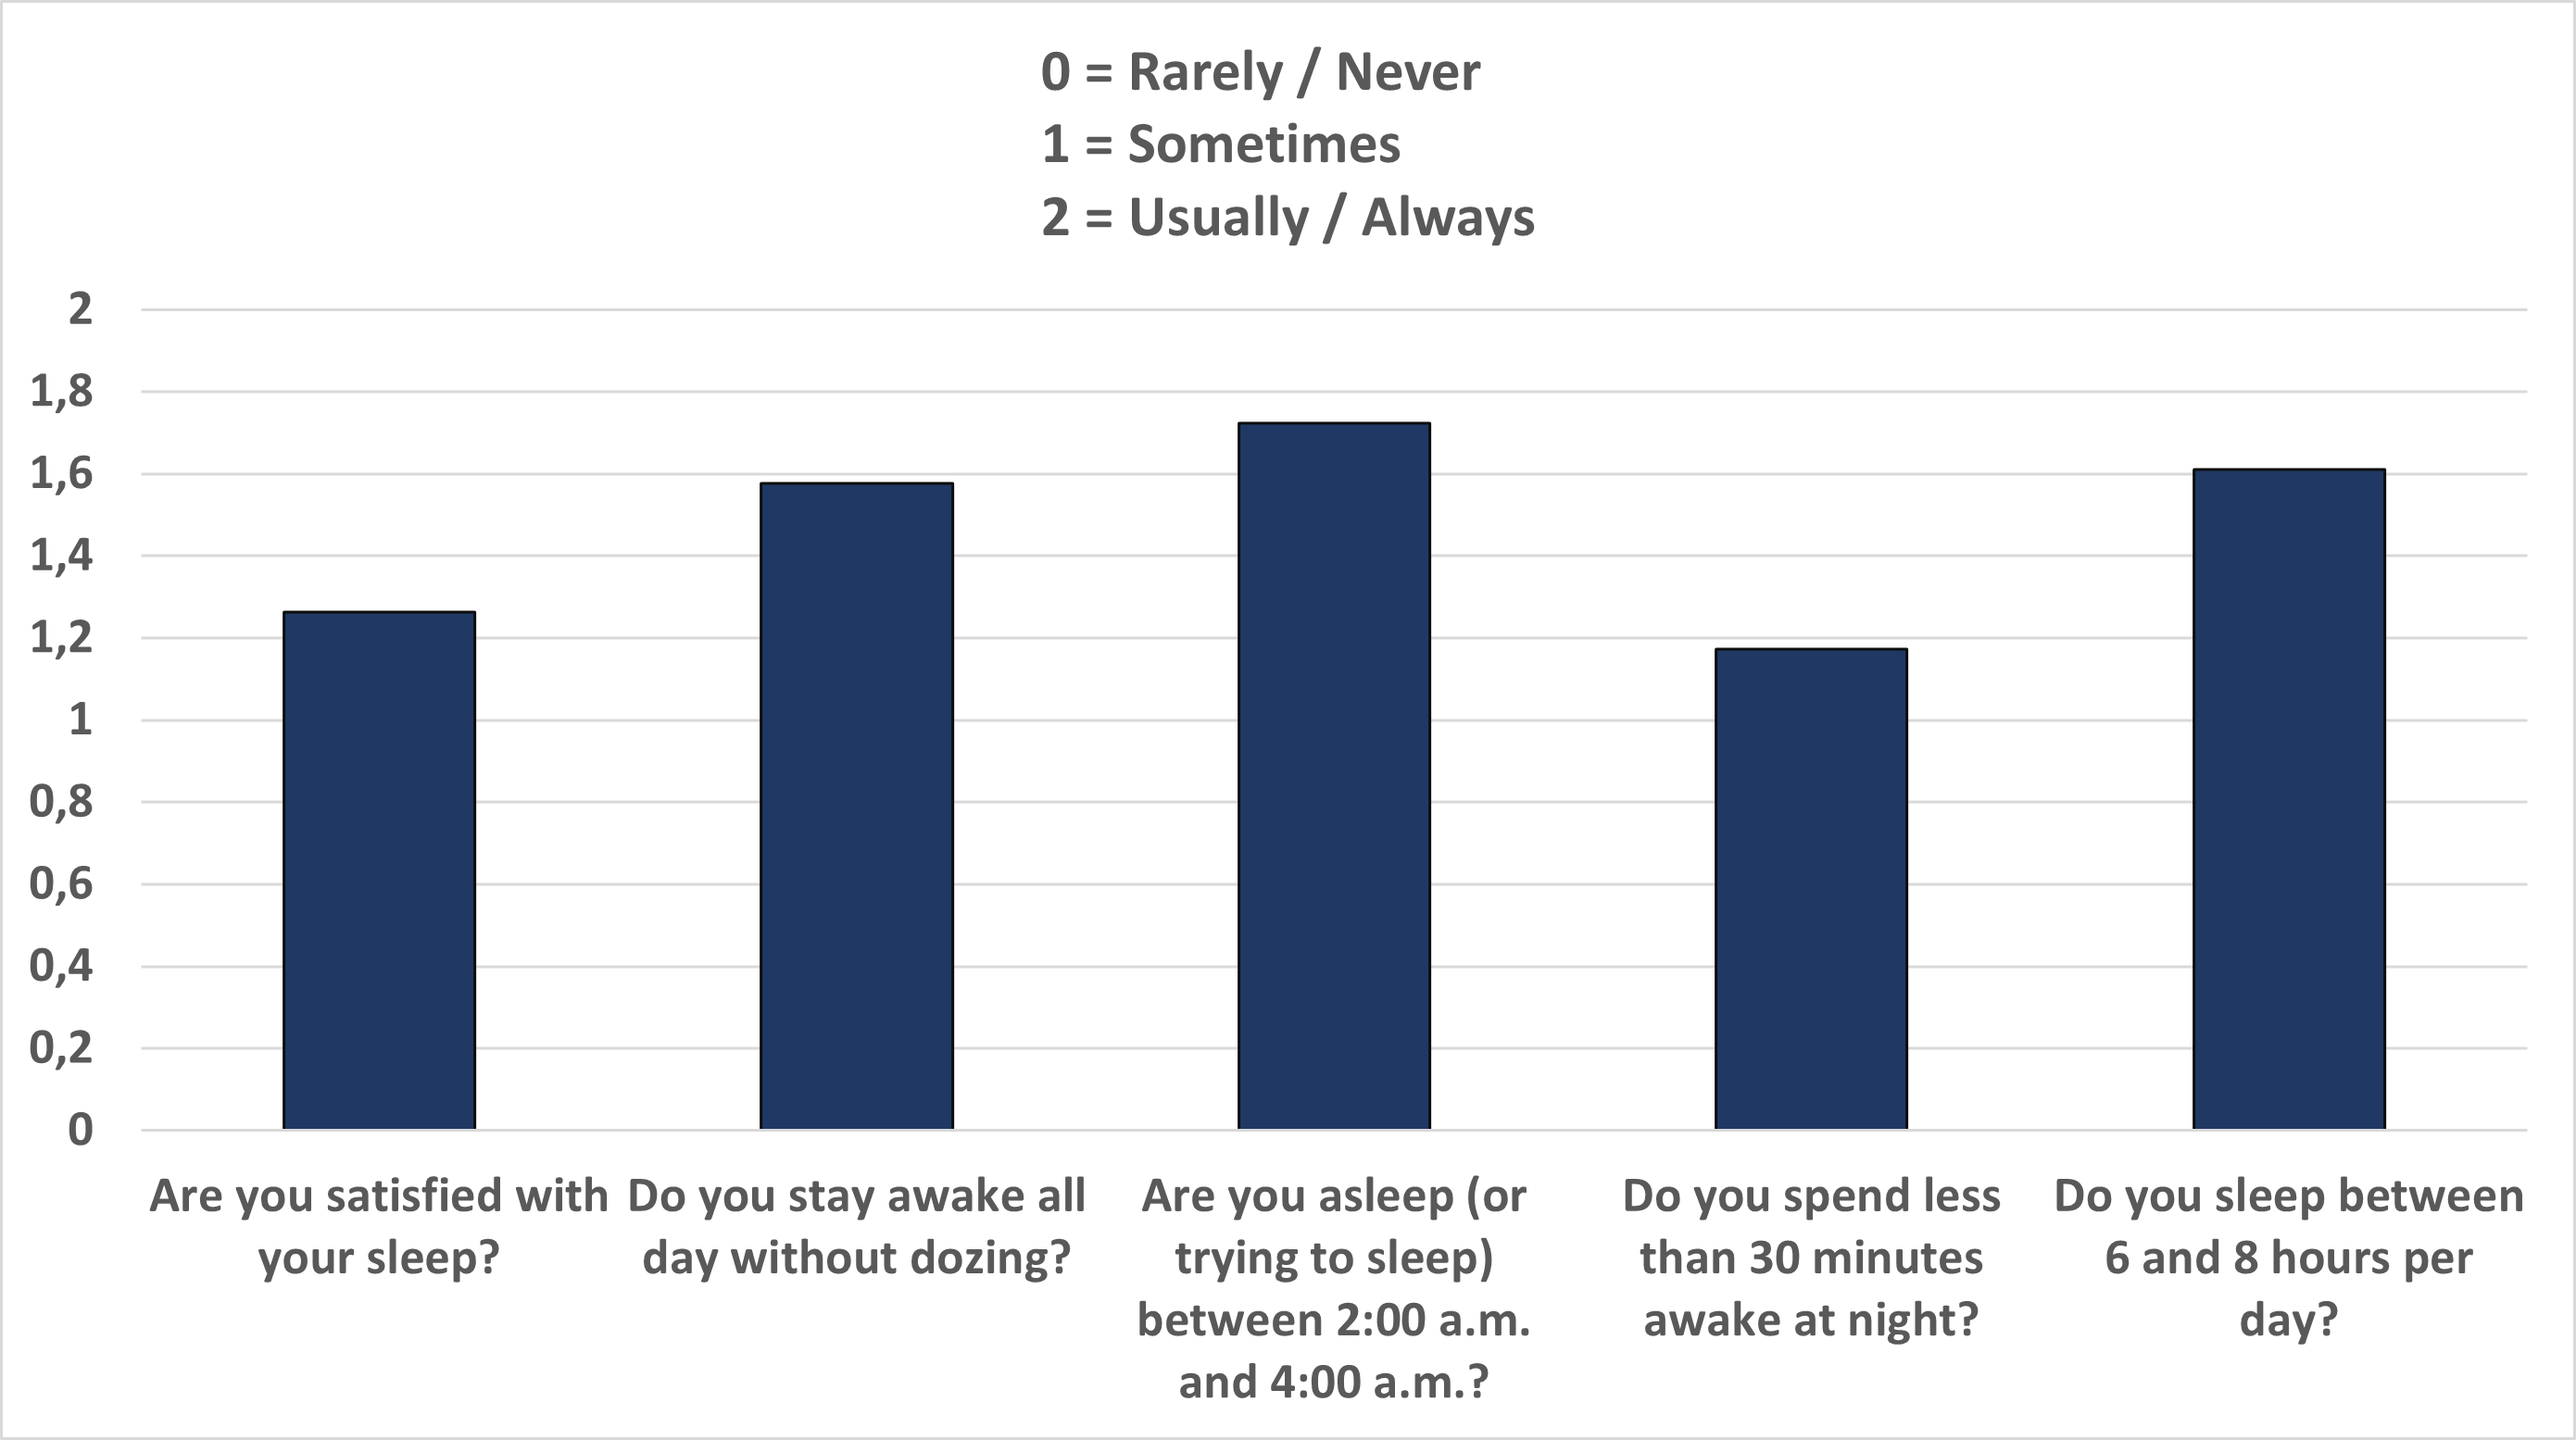
\includegraphics[scale=0.7]{graphics/SATED_Charts.png}
    \caption{SATED Questionnaire}
    \label{fig:SATED}
\end{figure}

\subsection{Sleep Tracking}
To comprehend how the participants use the present sleep tracking devices, we inquired about their usage habits and familiarity with them. The survey indicates a striking contrast in the usage of health trackers for monitoring sleep among participants. The majority of participants, 89 individuals, have never used sleep trackers before, while 30 former users stopped due to various reasons, such as a perceived lack of value, discomfort or forgetfulness. In contrast, 25 participants continue to find the use of these devices valuable for tracking their sleep.

\begin{figure}[H]
    \centering
    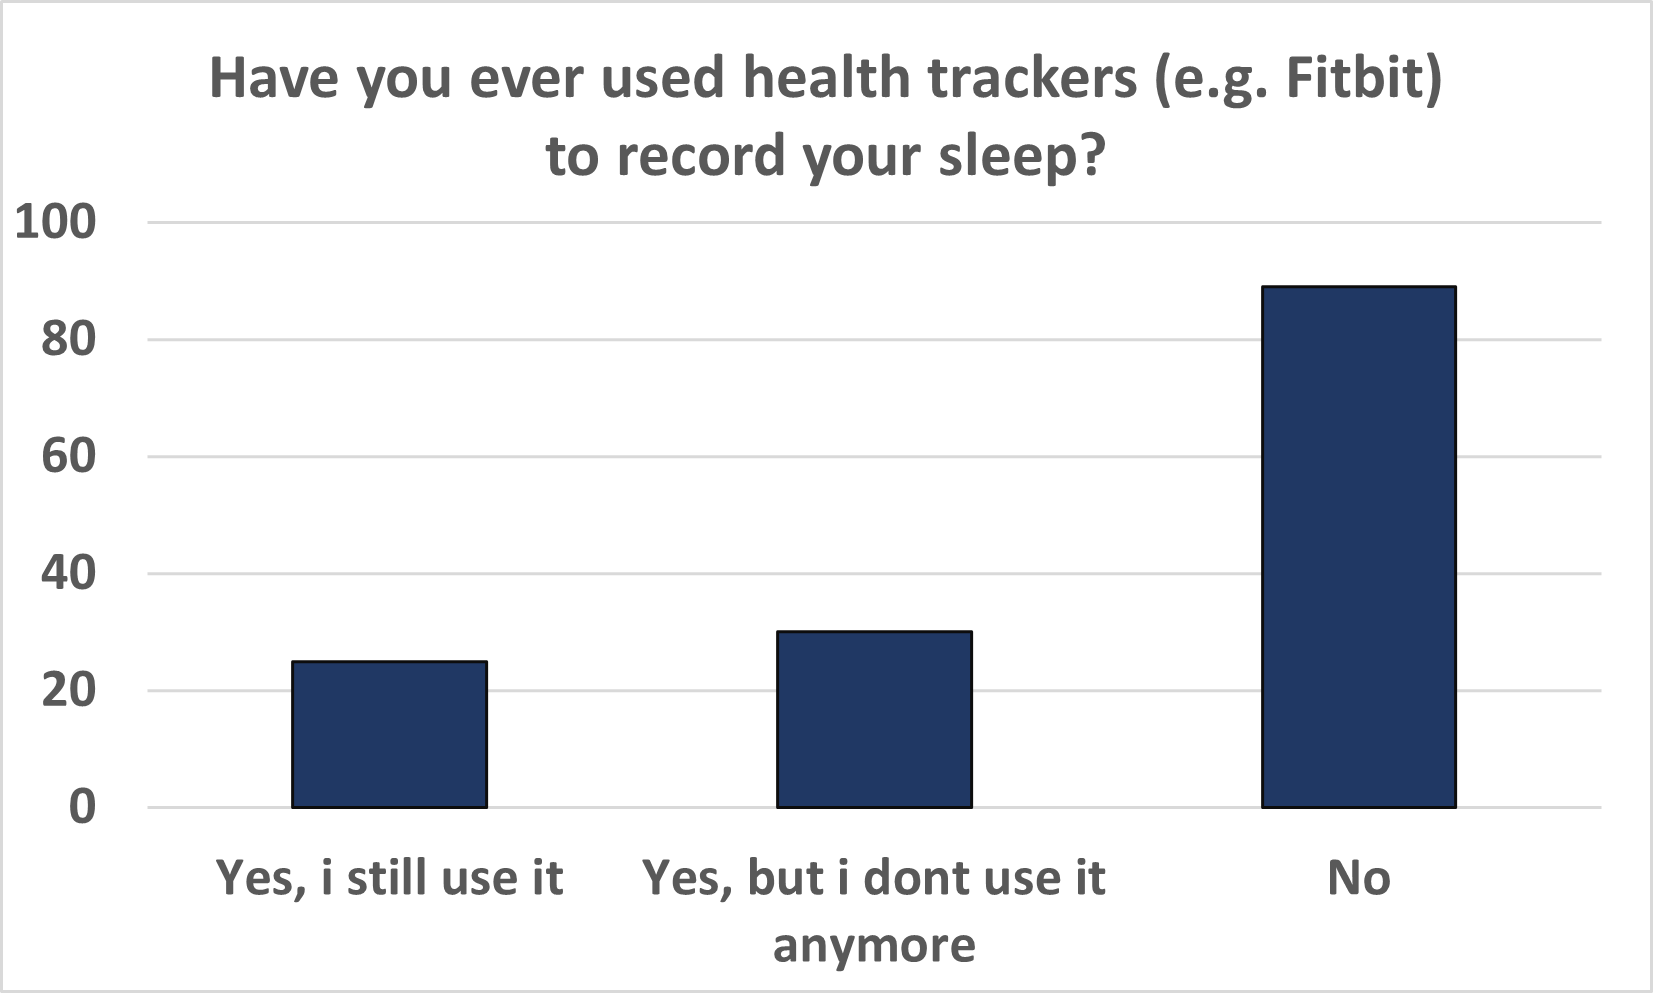
\includegraphics[scale=0.8]{graphics/Used_Sleep_Tracking.png}
    \caption{Sleep Tracking Experience}
    \label{fig:tracking_experience}
\end{figure}

\begin{figure}[H]
    \centering
    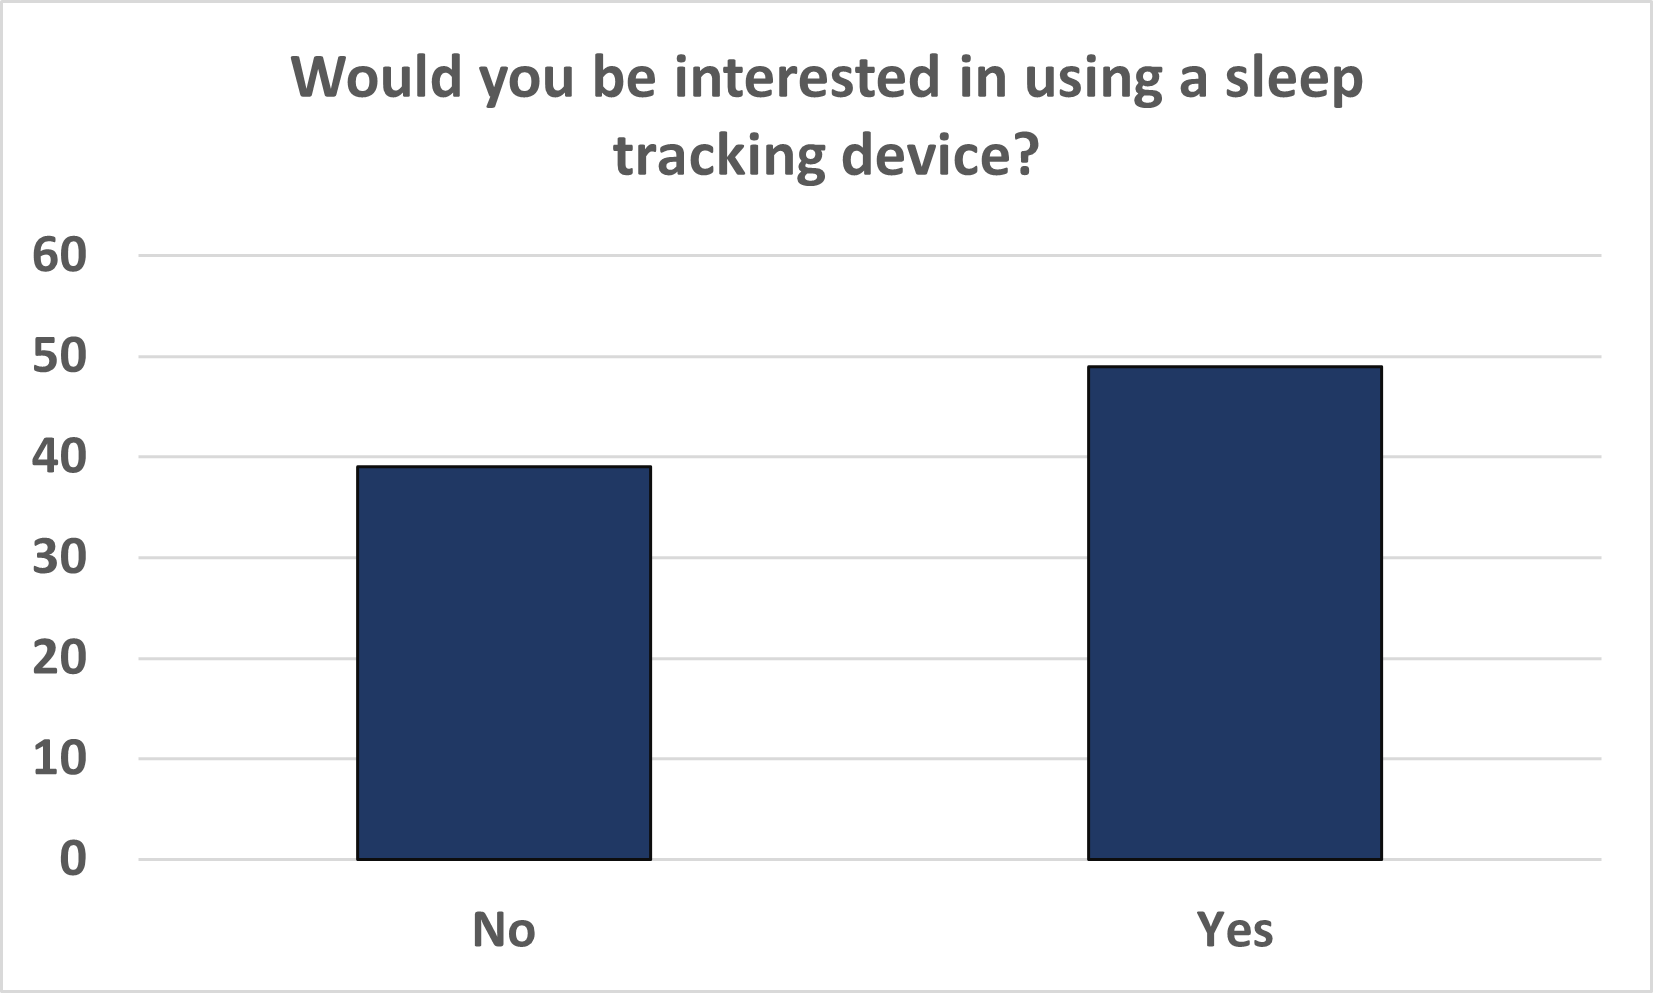
\includegraphics[scale=0.8]{graphics/Interested_in_Using.png}
    \caption{Interest in using a Sleep Tracker}
    \label{fig:interest_using}
\end{figure}

\paragraph{Non-Users Specific}
Those who chose not to use a sleep tracker (\autoref{fig:tracking_experience}) were asked if they would be interested in using one, showing that 49 people wanted to use a sleep tracker, while 39 did not (\autoref{fig:interest_using}). Reasons for rejecting a sleep tracker include feeling uncomfortable wearing it in bed, especially for those who already sleep well, concerns about privacy due to sharing data, including noise and medical records, and a dislike of technology because it may disrupt sleep or feel controlling.

\paragraph{Discontinued-Users Specific}
Participants who discontinued sleep tracking cited various reasons, including practical, technical, and personal factors. Common concerns were discomfort while sleeping and skepticism about the accuracy and usefulness of the data. Technical issues were related to device malfunctions and the need for frequent charging. Additionally, participants mentioned personal factors such as improved mental health, a desire to reduce nighttime technology use, and forgetting about the device.

\paragraph{Discontinued- and Continued-Users Specific}
The participants, categorized as Discontinuing and Continuing Users (\autoref{fig:tracking_experience}), were inquired regarding any enhancements in their sleep habits while utilizing sleep tracking. Out of the total respondents to this query, 38 participants reported no improvements while 17 affirmed improvements in their sleep habits through sleep tracking.

\begin{figure} [H]
    \centering
    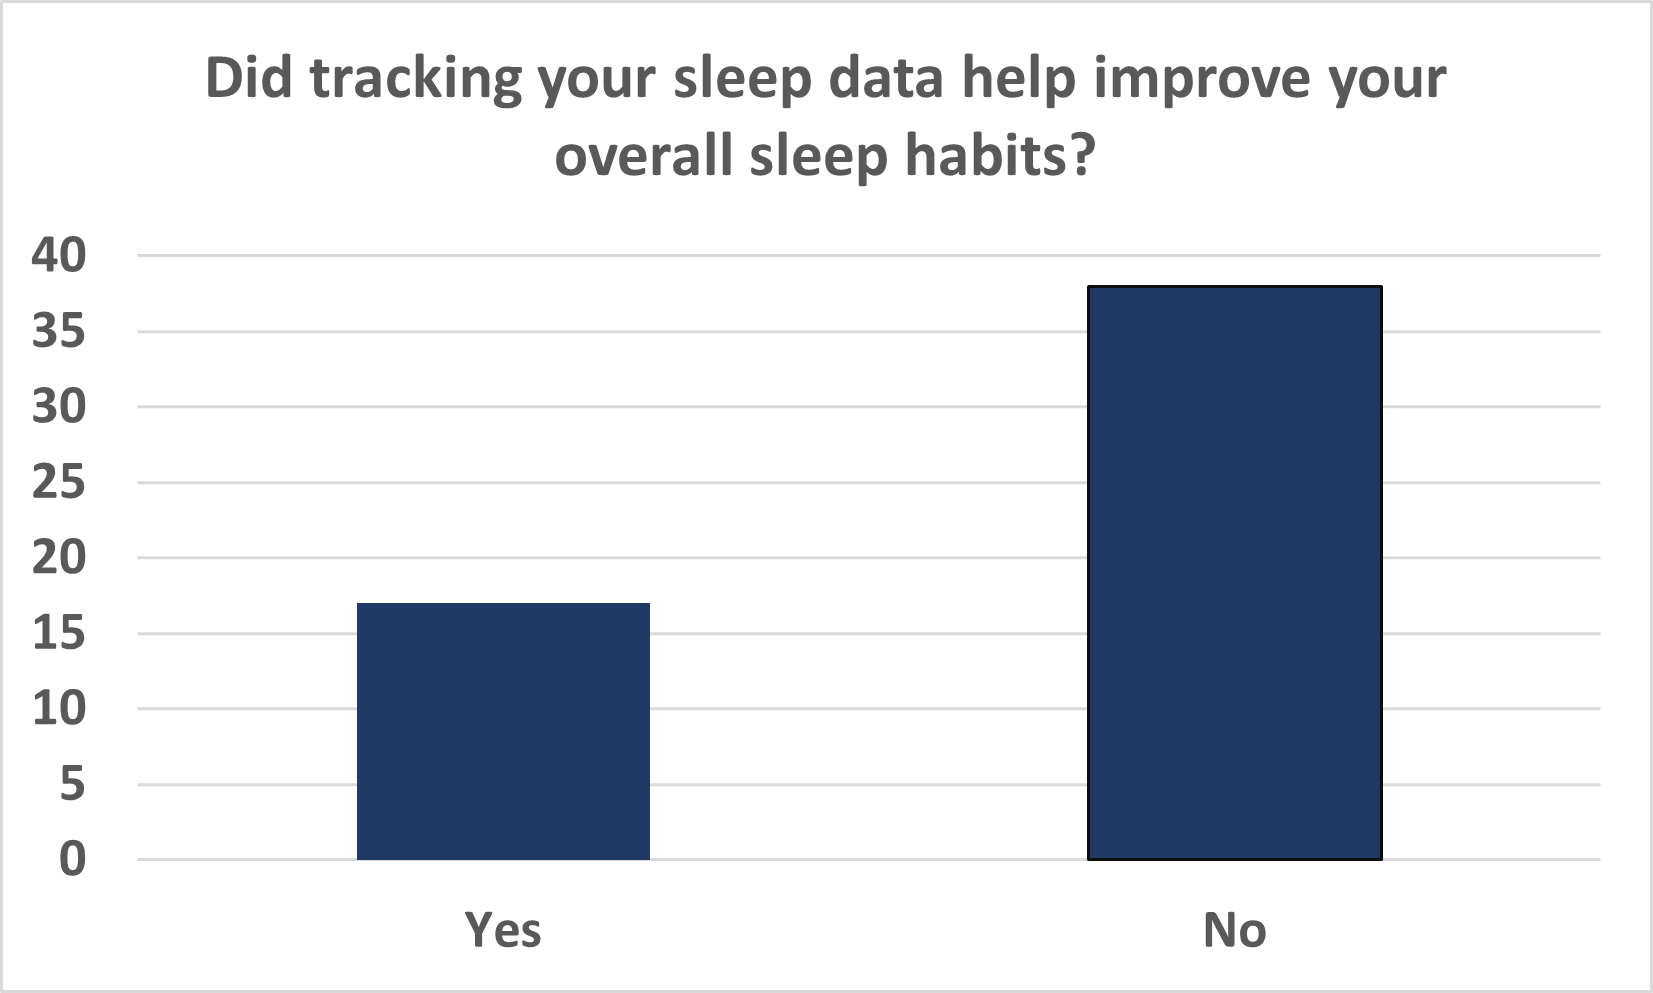
\includegraphics[scale=0.8]{graphics/Tracking_Improve.png}
    \caption{Improvement through Sleep Tracking}
    \label{fig:improvement}
\end{figure}
Participants who \textbf{did not} see sleep improvements with trackers mainly used them for information, not for sleep enhancement. They often lacked motivation to change sleep habits and expressed doubts about data accuracy, sometimes misinterpreting stillness as sleep. Factors like noise, temperature, discomfort from the tracker, and sleep anxiety impeded sleep quality improvement. The trackers failed to provide practical guidance, leading some to find no beneficial changes in their sleep routines despite knowing their patterns. Inconsistencies in tracking and perceived low value from the data further limited their effectiveness.

Participants who \textbf{did} observe sleep improvements with trackers also noted several limitations. Technical issues like short battery life affected tracking effectiveness, and the need for manual alarm or sleep time settings each night was inconvenient. Forgetting to activate the device was a common oversight. While trackers raised awareness of sleep patterns, they didn't significantly change sleep duration or timing for most.

\begin{figure} [H]
    \centering
    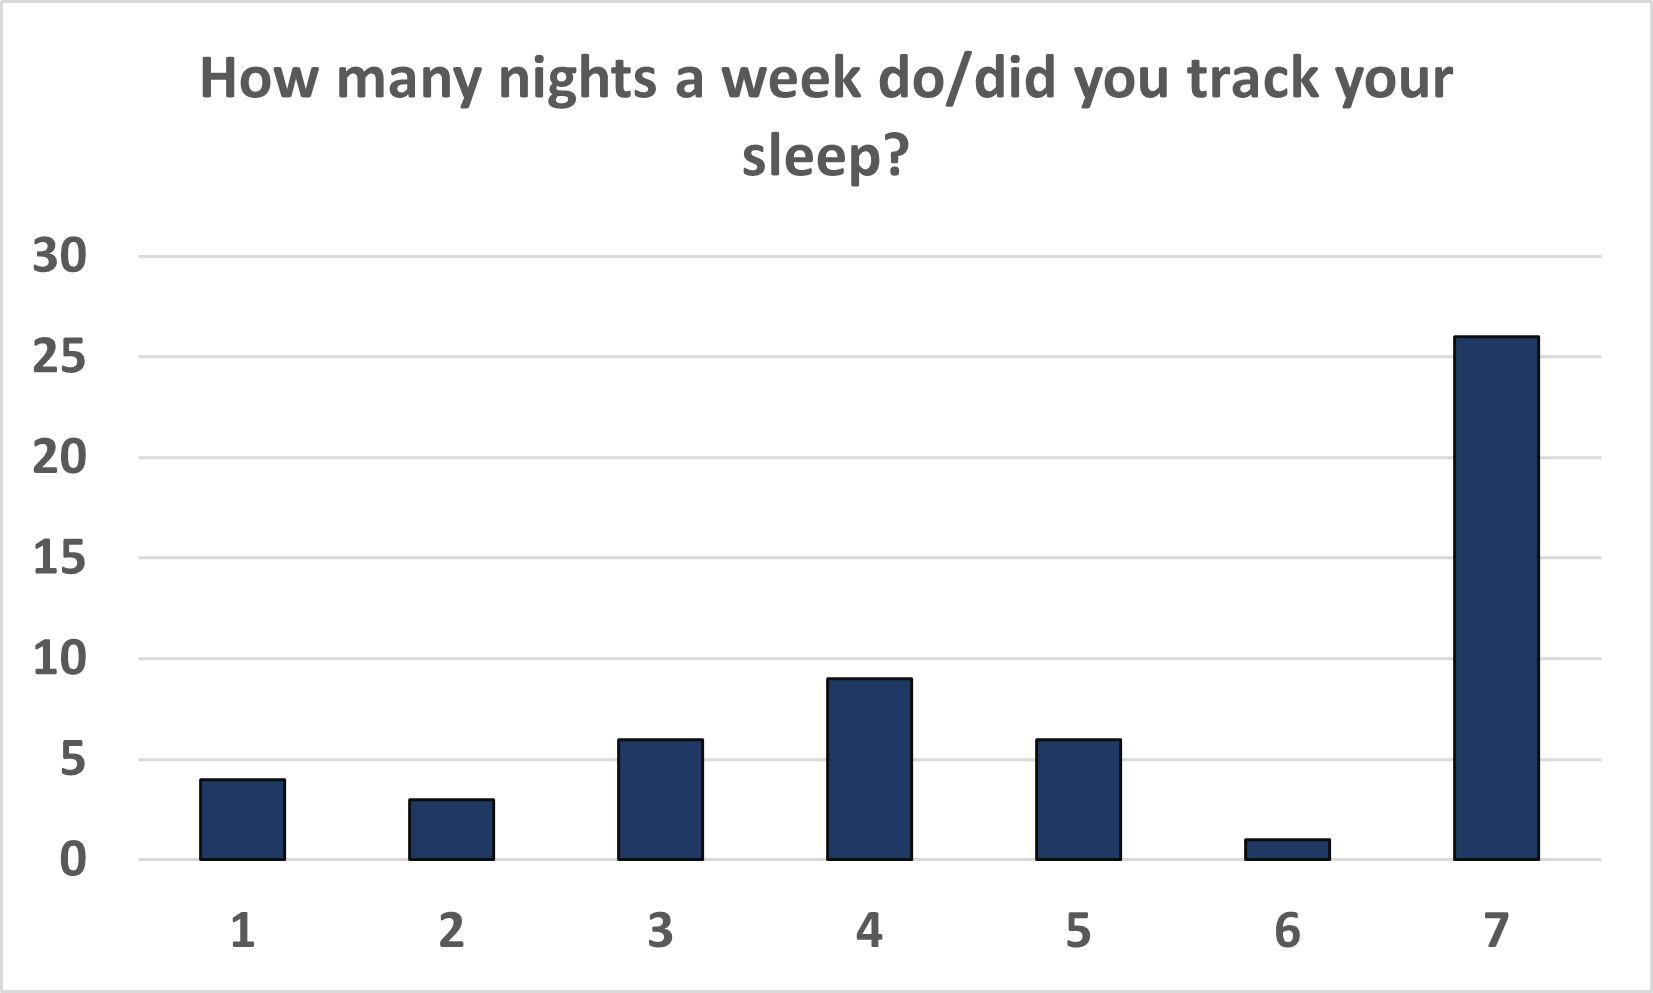
\includegraphics[scale=0.8]{graphics/How_Many_Nights.png}
    \caption{Weekly Tracking Frequency}
    \label{fig:weekly}
\end{figure}

The majority of participants (26) used a sleep tracker daily, while those using it less than 5 nights a week (22) cited various reasons for lower frequency. Device-related issues, especially battery life, frequent charging needs, and discomfort, hindered daily usage. Forgetting to use or activate the tracker suggested a lack of creating a new habit or perceived immediate benefit. The absence of noticeable help or benefits from the tracker reduced motivation for regular use.

\begin{figure}[H]
    \centering
    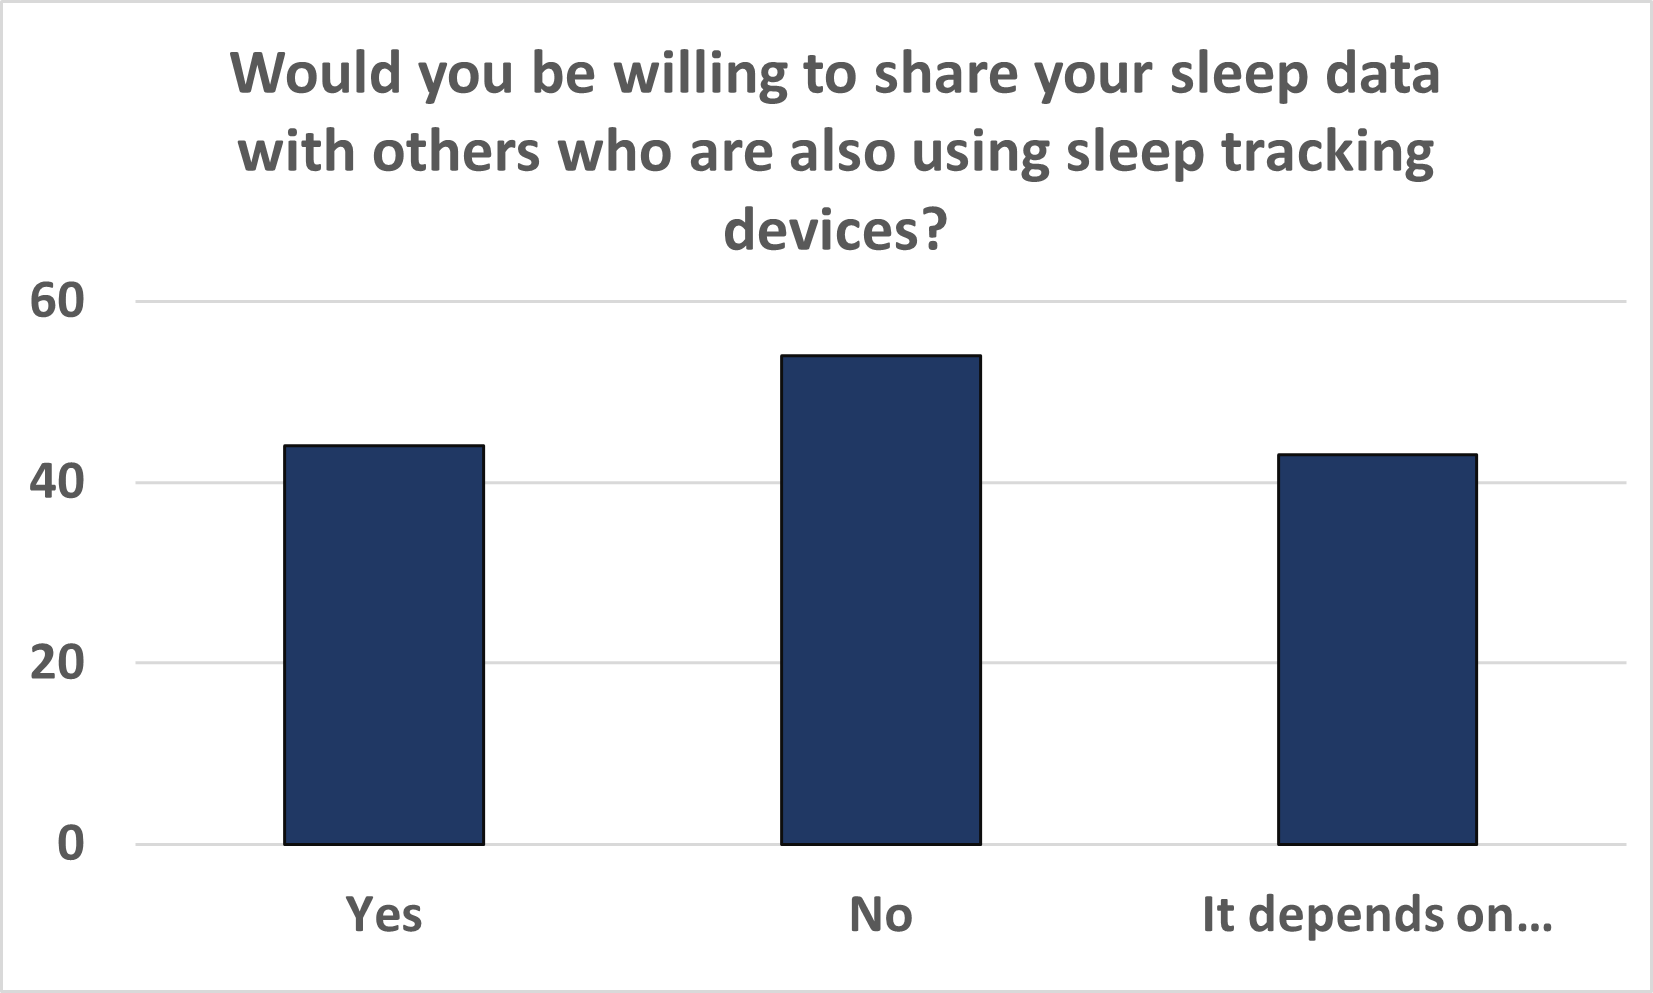
\includegraphics[scale=0.8]{graphics/Share_Data.png}
    \caption{Share Sleep Data}
    \label{fig:share}
\end{figure}

Lastly for the section of sleep tracking, all participants were asked about their willingness to share their sleep data with others. 

Participants who \textbf{did not} want to share sleep data cited privacy concerns, viewing sleep as personal and fearing data misuse. They preferred anonymous data sharing, if necessary.  Additionally, some worried about the negative impact on sleep quality from sharing. There was a general disinterest in sharing or comparing sleep data, with doubts about its value or personal benefit.

Participants who chose \textbf{"It depends on..."} value anonymity, often agreeing to share for scientific or medical reasons if their identity is protected. They're more willing to share with trusted individuals like close relations or medical professionals than unknown entities. Concerns about secure data handling and privacy regulations are prominent. Some are comfortable sharing only statistical or aggregated data.

\subsection{Object Design Preferences}
\begin{figure} [H]
    \centering
    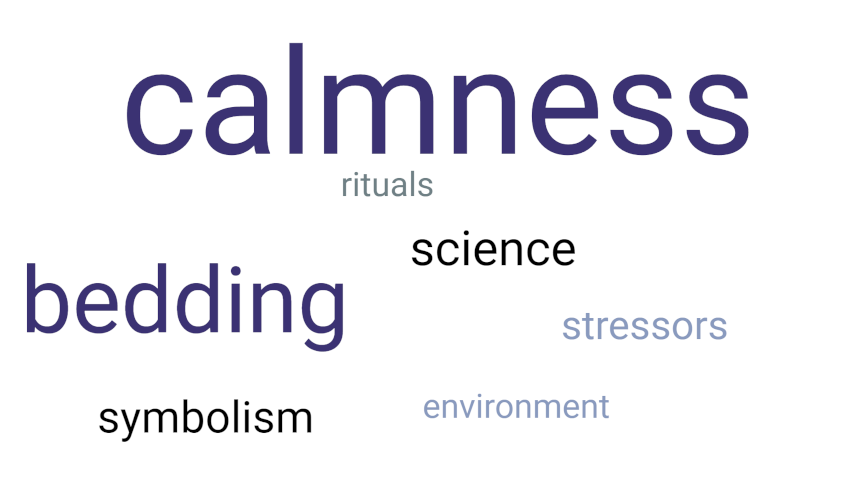
\includegraphics[width=\paperwidth/2]{graphics/word-cloud_Things_resize.png}
    \caption{Word-Cloud Things / Concepts}
    \label{fig:things}
\end{figure}
In this section, participants were presented with questions related to the design of a physical object representing sleep data. The question "What thing(s)/concept(s) do you associate most with sleeping?" resulted in a large variety of different ideas, which are categorically displayed on a word-cloud (\autoref{fig:things}). One of the most frequently occurring things was the "bed" (27), which is part of the "bedding" category, together with entries like "pillow" (5) or "mattress" (3). The biggest category "calmness" had mostly occurrences like "rest" (10), "relax" (13), "quiet" (8) or "recovery" (6).

\begin{figure} [H]
    \centering
    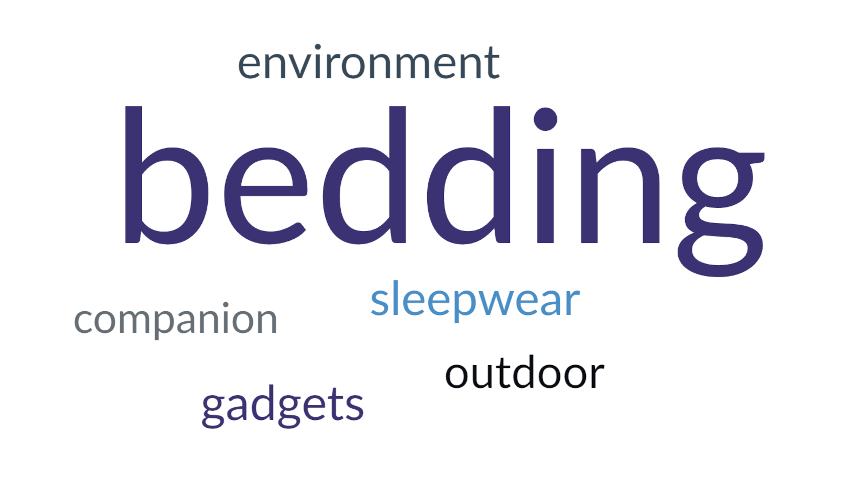
\includegraphics[width=\paperwidth/2]{graphics/word-cloud_physical_resize.png}
    \caption{Word-Cloud Physical Object}
    \label{fig:physical}
\end{figure}

The following query "What physical object(s) do you associate most with sleeping?" resulted primarily in entries of the category "bedding", as shown in the word-cloud (\autoref{fig:physical}). The word "bed" had a total count of 72, followed by pillow with 46.

In the next set of questions the participants were asked to imagine an object, capable of physicalizing sleep data, and answer the questions based on that object. The participants particularly valued the representation of sleep quality (110), sleep duration (77), and sleep stages (142) as the most important types of sleep data that the device should track. The most expected insights to gain from the object were understanding sleep quality and efficiency (97), identifying sleep disturbances or disruptions (89) and increasing self-awareness of sleep habits (83). Both questions allowed multiple selections. The imagined object was mostly preferred as interactive (95) instead of static (34) and should be able to represent the sleep data both ranging from daily to weekly (61). The preferred method of initial interaction between the user and the device was predominantly touch-based (87), with light indicators as the second choice (43). The interaction between the user and the object was again preferred to be touch-based (118). Participants also liked the object to be portable (92), instead of stationary (36) and predominantly wanted it to be placed beside their bed (99).



\begin{figure}[H]
  \centering
  \begin{minipage}[b]{0.45\textwidth}
    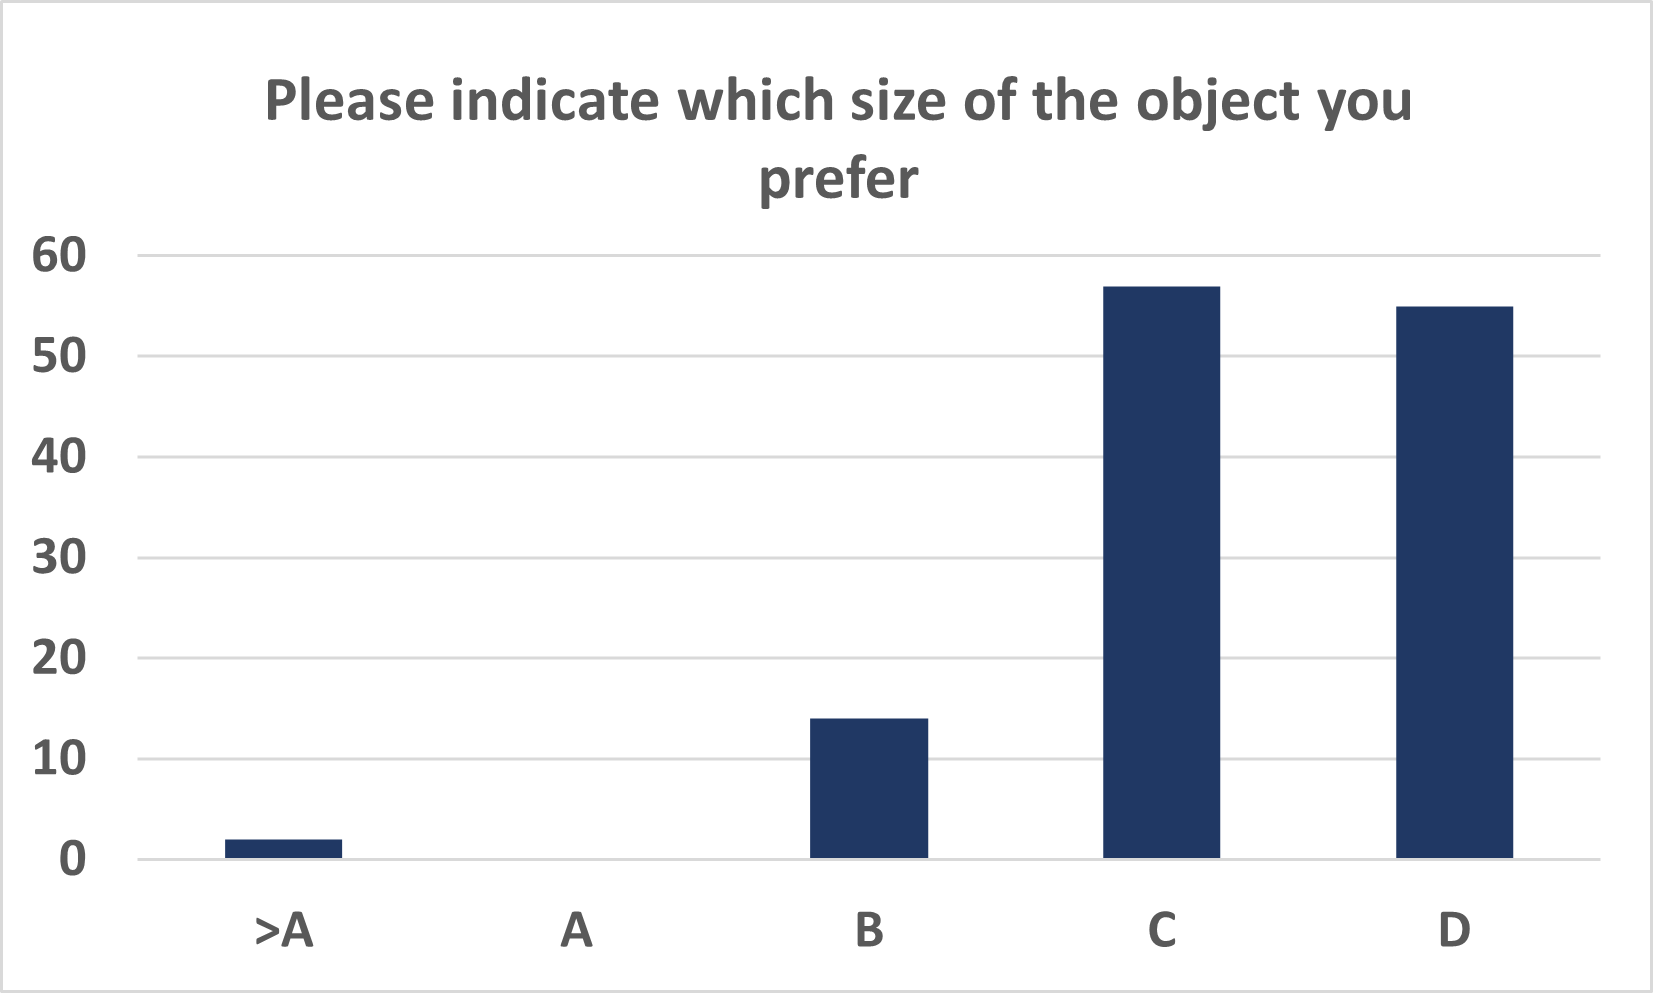
\includegraphics[width=\textwidth]{graphics/Size.png}
    \caption{Preferred Object Size}
    \label{fig:size-selection}
  \end{minipage}
  \hfill
  \begin{minipage}[b]{0.45\textwidth}
    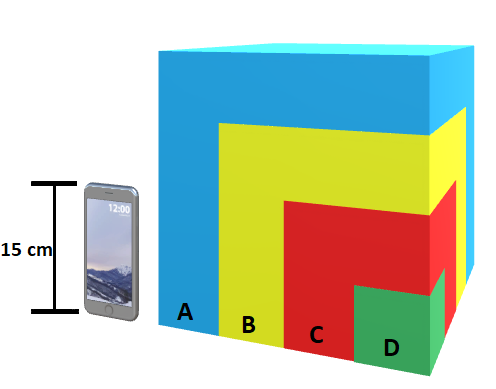
\includegraphics[width=\textwidth]{graphics/Sizeselect+prototype.png}
    \caption{Size Selection}
    \label{fig:size}
  \end{minipage}
\end{figure}

For the last question of the online survey, participants mostly preferred the object to be rather "smartphone-sized", as shown in \autoref{fig:size-selection} and \autoref{fig:size}.


\section{Online Survey Discussion}
This chapter details how the analysis of existing studies and theories, and the study results, were employed in the development
of the tangible prototype concept. The structure follows the research questions presented earlier.

\paragraph{What categories of sleep data are relevant for effective visualization and understanding?} Given that sleep habits and overall sleep health vary greatly from person to person and are not yet fully comprehended \cite{Define_Sleep_Health}, identifying the relevant variables in sleep data was crucial for obtaining qualitative insights from the prototype. Because the actual data representation would alter the object's visual design \cite{Oppotunieites_Challenges_DataPhysicalization}, it was essential to address RQ1 before proceeding with the design process. 
\begin{figure}[H]
    \centering
    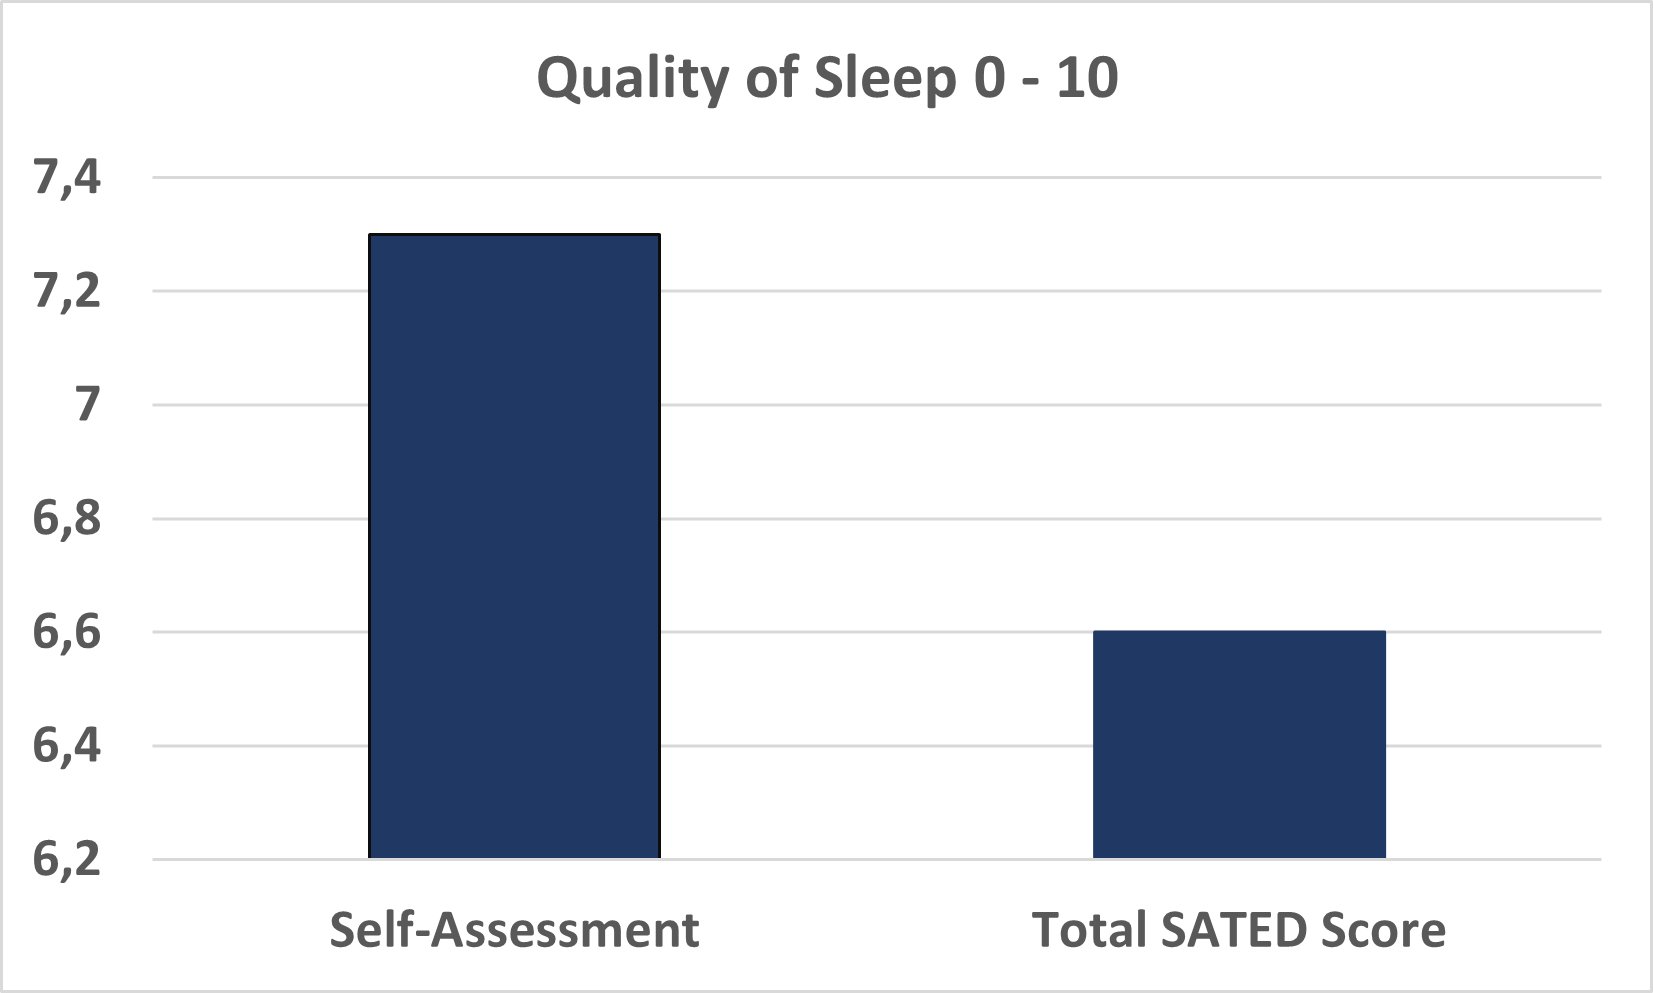
\includegraphics[scale=0.8]{graphics/SATED_vs_Self.png}
    \caption{Self-Assessment and Total SATED Score}
    \label{fig:self}
\end{figure}
The comparison of the self-assessment and the overall SATED-score (\autoref{fig:self}) show a discrepancy in the evaluation of ones sleep quality, which could offer potential for using an overall sleep quality-score as a relevant data metric. In addition to the results of the object design preferences, we decided to primarily use sleep quality, sleep duration, and sleep stages as a relevant data metric for our prototype, since those variables were most anticipated by the surveys participants and are also mostly used in other consumer sleep tracking methods \cite{Consumer_SleepTracking}. The preference of the majority for the capability to analyze both daily and weekly data led to its incorporation into the design phase. This approach is akin to the use of historical data in ambient designs, which has been shown to boost user motivation for specific actions \cite{rodriguez_cammina_2013}.

\paragraph{How should a physical prototype that communicates sleep data look?}
The survey results underscore an importance of "calmness" (\autoref{fig:things}) in the context of sleep, suggesting a design approach that prioritizes the creation of a serene and restful atmosphere. The presence of "bedding" in both word-clouds (\autoref{fig:things}, \autoref{fig:physical}) together with the preferences towards a touch-based interaction are indicating towards tangible elements.
The preference of having an interactive object opens an opportunity for dynamic physicalizations, which leads to data encoding in form of behavioral changes of the physical representation \cite{Representation_Modality_Data_Artifacts,Oppotunieites_Challenges_DataPhysicalization}. Comparing the results from the \textbf{Discontinued-Users}, \textbf{Continued-Users}, and the participants who were tracking less than 5 days a week, experienced no benefits or help from the tracker, leading to decreased motivation, ultimately suggesting that motivation is a key issue, which was mentioned in studies before \cite{Stage_Based_Model, Challenges_Oppotunieties_SleepTracking}. This implies that an alternative approach, such as ambient representation, could improve motivation by making data easier to comprehend with less effort required from the user.

\paragraph{How should a physical prototype communicate sleep data?}
The survey results gave a clear direction towards a touch-based interaction and communication between the user and the object. In the realm of data physicalization, a touch-based interaction doesn't necessarily have to be an interaction via a touch-screen, it also can be the sensation of feeling temperature or surface changes of an object \cite{Oppotunieites_Challenges_DataPhysicalization}. The survey question about the preferred ways of communication also offered a few limitations, since the majority of participants are very familiar with the use of a touch-screen, which could have led to a biased decision. Keeping that in mind and also considering the amount of participants preferring light-indicators as form of communication, they could pave the way to have a comforting ambient visualization which incorporates a certain "calmness" by using calming light effects.

\chapter{Focus Group}
As the online survey still had a few ambiguities and no clear object or communication method emerged, we decided to hold an additional focus group. This focus group was intended to provide a clearer direction for our prototype by actively creating objects and to provide a comparison with the results from the online survey.
\section{Method}
For the focus group, participation was open and unrestricted, mirroring the approach taken for the online survey. Upon completion of the online survey, participants were given the opportunity to indicate their interest in future studies. Those who opted in provided their email address, which we used to send invitations to the focus group. A subset of these participants chose to attend.
\subsubsection{Participants}

\begin{table}[h]
\centering
\begin{tabular}{|c|l|}
\hline
\textbf{Participant} & \textbf{Professional Background}                                          \\ \hline
1                    & Researcher in software engineering with a focus on machine learning       \\ \hline
2                    & Individual with recent research experience at an alternative academic institution \\ \hline
3                    & Research assistant affiliated with a different academic department        \\ \hline
4                    & Researcher engaged in projects at the human-centered ubiquitous media chair \\ \hline
5                    & Student with personal experience in managing sleep disorders              \\ \hline
6                    & Doctoral candidate active in the human-centered ubiquitous media department \\ \hline
\end{tabular}
\caption{Academic and Professional Backgrounds of Focus Group Participants}
\label{tab:participants_background}
\end{table}

\subsubsection{Survey Content}
Participants were actively encouraged to work together with tools to create or design a prototype that corresponds to their ideas of implementing a physical visualization of sleep data. The participants were divided into three groups and after a short introduction they had about 30 minutes to develop a prototype. To help them, the participants were given some sleep tracking variables to use, such as sleep duration, sleep quality and sleep stages, which were also the most requested variables from the online survey. Of course, the participants were also allowed to use their own variables. As additional support, a guiding form was used, which, with the help of some specific questions regarding the prototype, could help to develop a well thought-out design.
\section{Focus Group Results}

\textbf{Group 1} presented a docking station designed to blend into the bedroom environment and to act as a sleep stage indicator and gentle wake-up light. The complementary element, conceived as a portable object, would provide a tangible representation of sleep quality and act as a stress relief toy. The squishiness of this object would indicate sleep quality, with additional playful elements such as a ball and cup game function. The thread connecting the ball to the cup represents sleep duration; its length varies according to the users sleep duration, making the game unplayable if the sleep duration was too short.

\begin{figure}[H]
  \centering
  \begin{minipage}[b]{0.4\textwidth}
    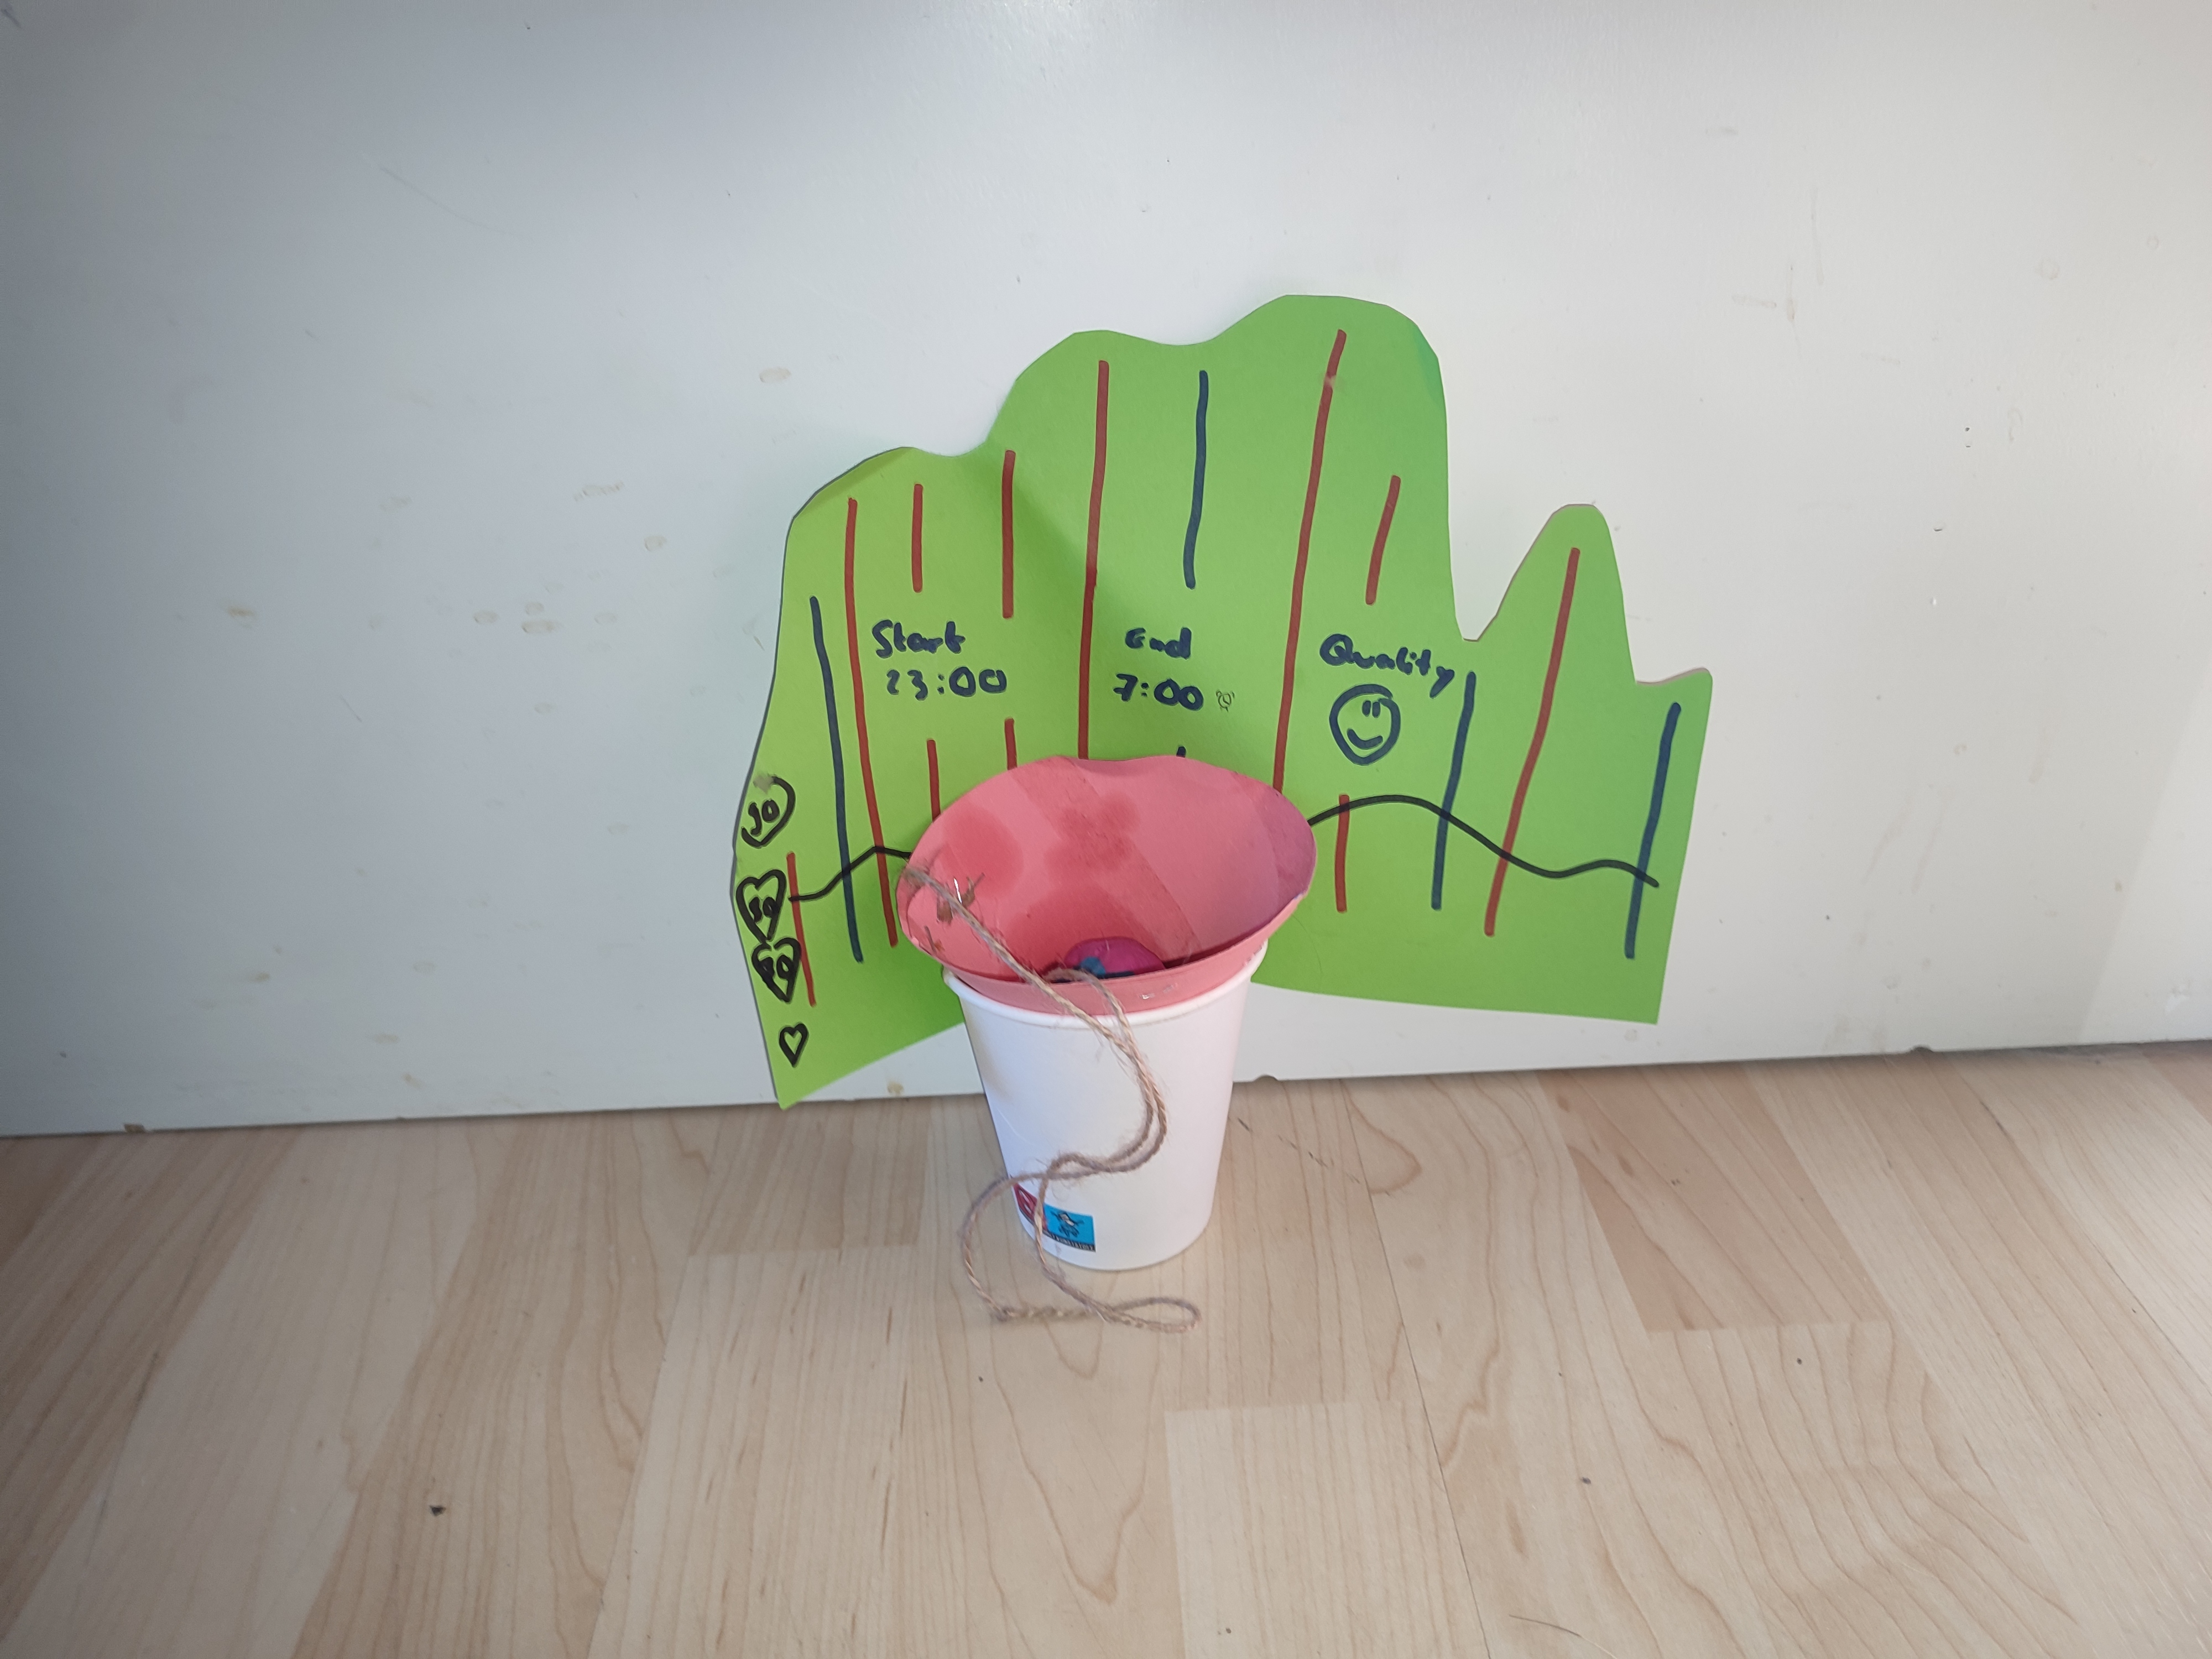
\includegraphics[width=\textwidth]{graphics/FocusGroup1.jpg}
    \caption{Prototype docked}
  \end{minipage}
  \begin{minipage}[b]{0.4\textwidth}
    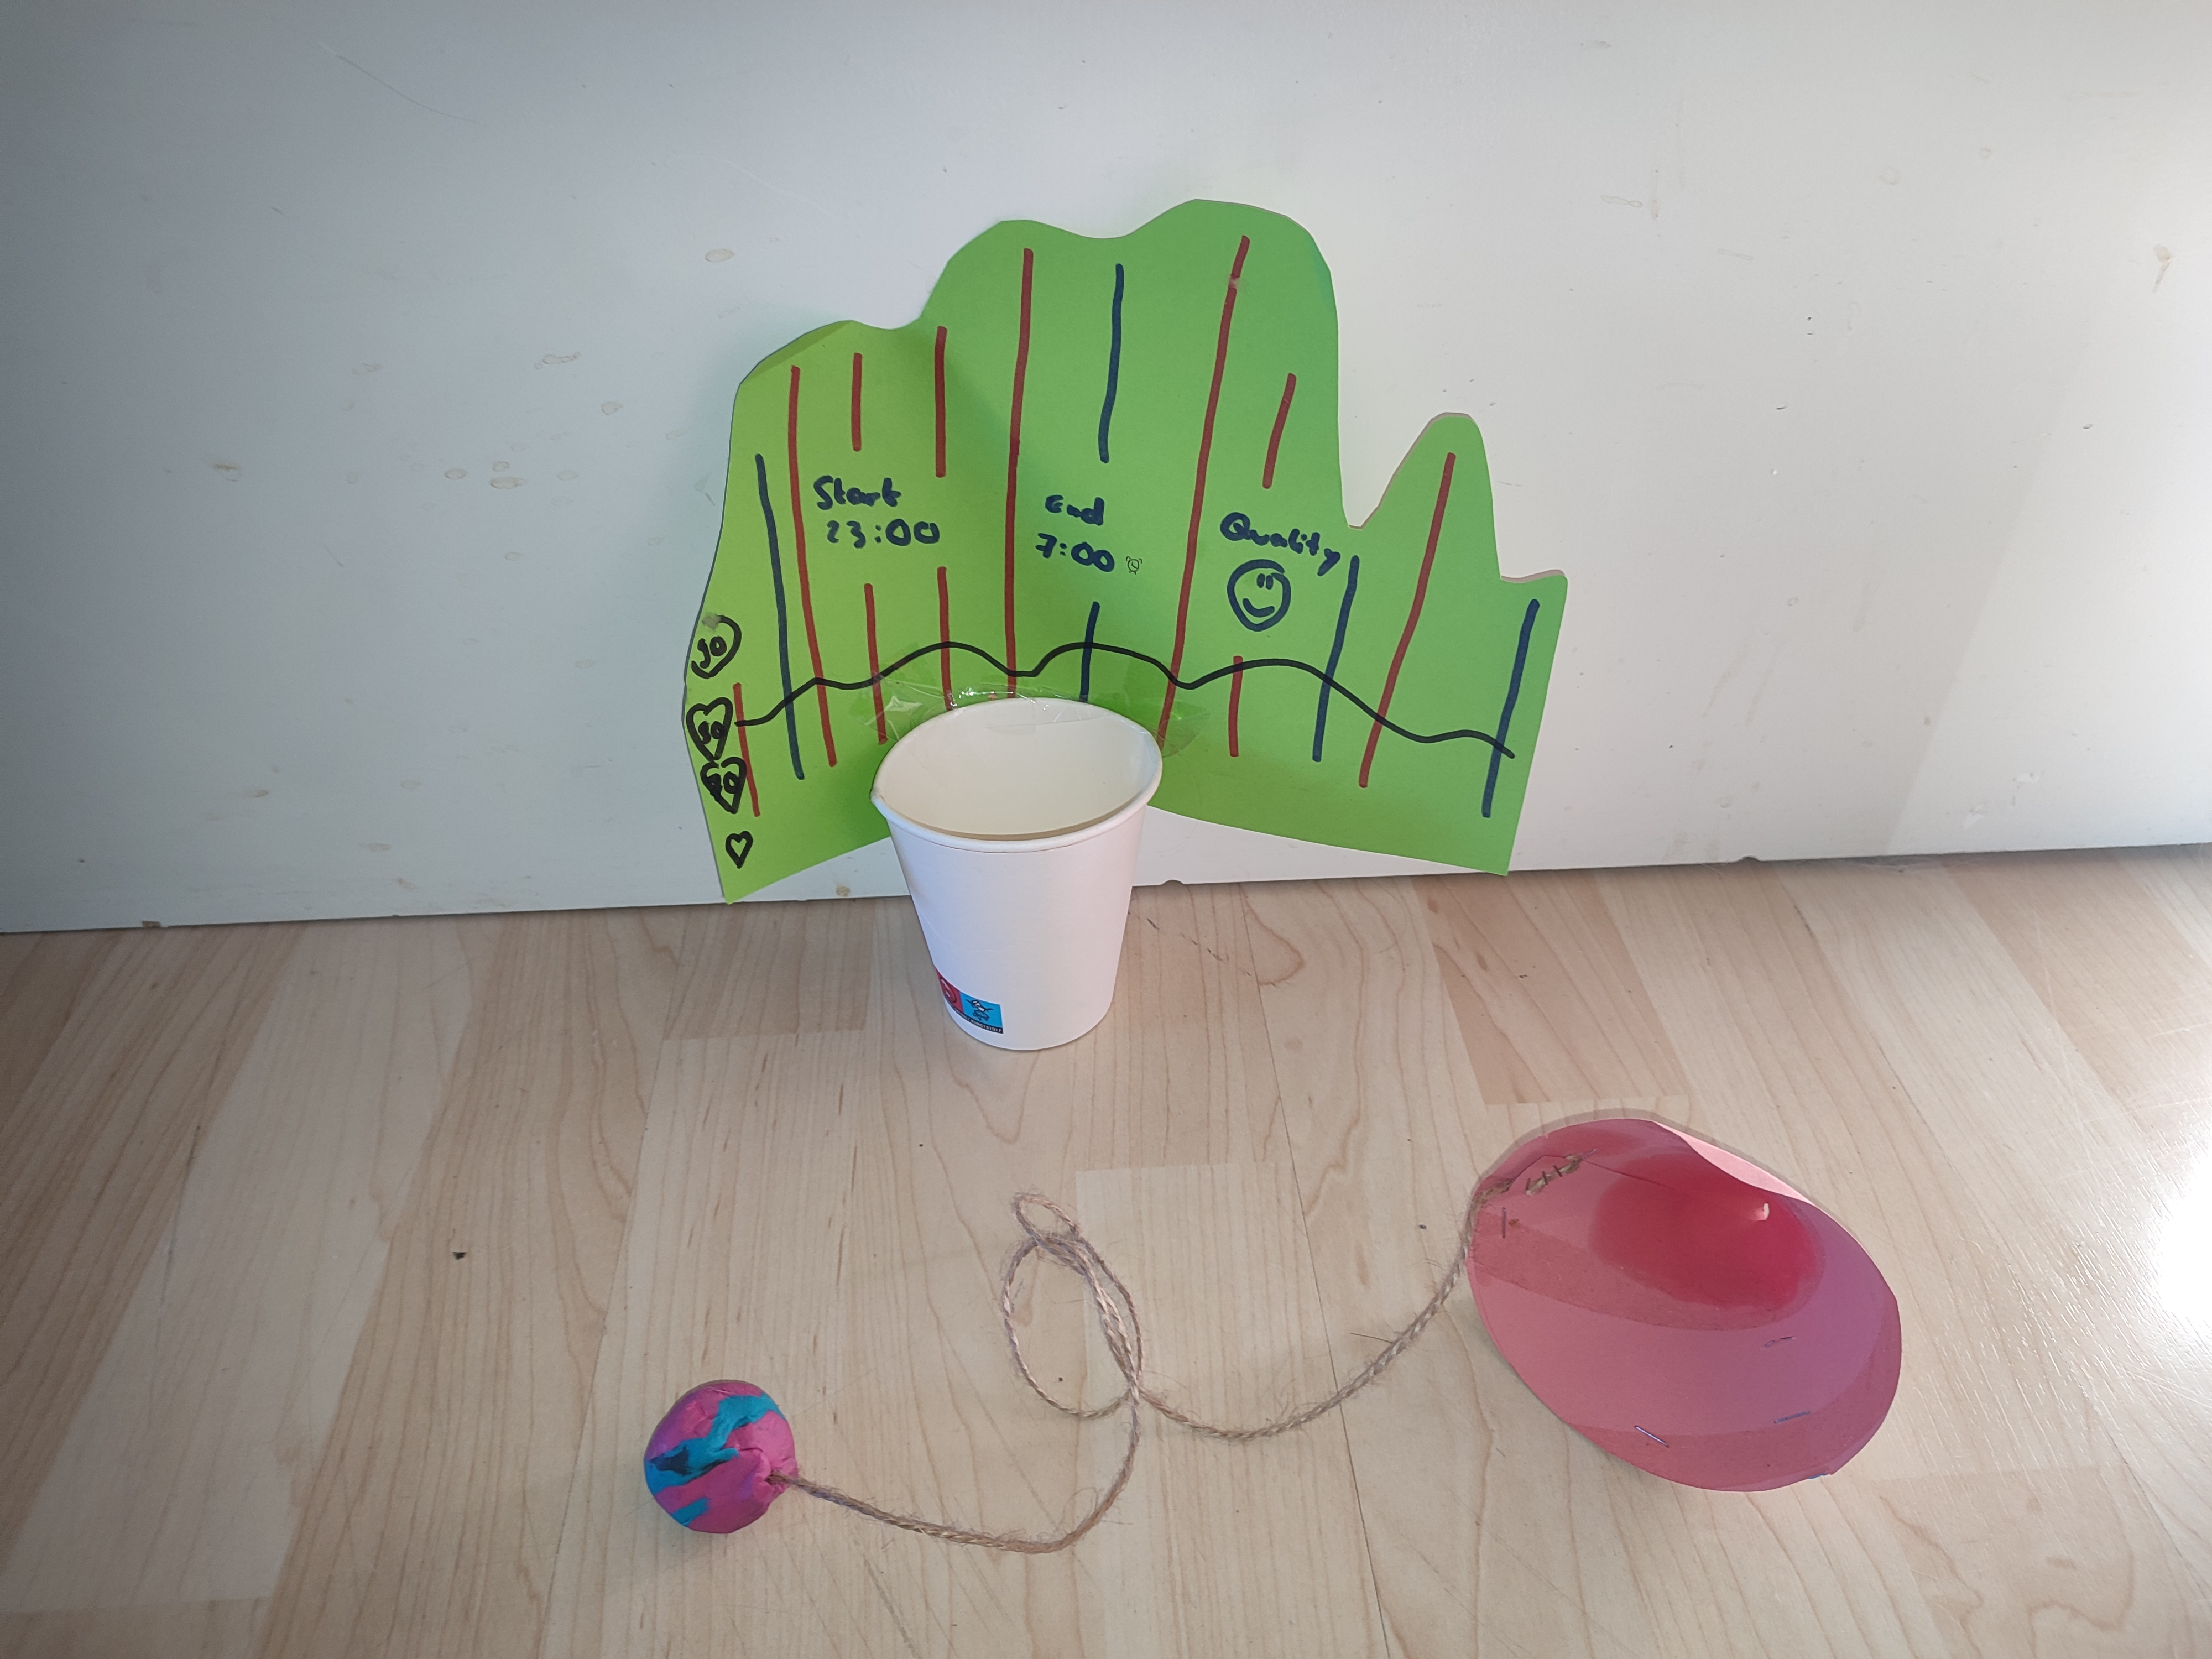
\includegraphics[width=\textwidth]{graphics/FocusGroup1_2.jpg}
    \caption{Prototype undocked}
  \end{minipage}
\end{figure}

\textbf{Group 2} proposed a sleep tracker integrated with an alarm clock that could project sleep data onto the wall. This concept included a color-coded sleep score and an interactive display that provided a summary of sleep patterns, duration and quality metrics such as heart rate variability.

\textbf{Group 3} presented an interactive design resembling a 3D bed with a clock that deforms to illustrate sleep quality over time, suggesting an interaction through manual rotation of the pointer to reveal different sleep events. Also, while turning the clocks pointer to a certain timestamp, the clock's form alters to reflect the user's sleep position at various times.

Notes and sketches done during the Focus Group can be found in the \autoref{appendix:appendix_A}.

\section{Focus Group Discussion}

\paragraph{What categories of sleep data are relevant for effective visualization and understanding?}
The focus group creations highlighted the importance of sleep duration, sleep quality and sleep stages as the primary categories of data relevant to visualization. This aligns with the earlier preferences expressed in the online survey, suggesting these metrics are not only fundamental but also the most sought-after data points for users interested in sleep wellness. The inclusion of additional metrics such as heart rate variability was also suggested to enhance sleep wellness. 

\paragraph{How should a physical prototype that communicates sleep data look?}
The designs in Groups 2 and 3 suggest that subtlety in the environment, such as a clock or ambient display, is preferred for a constant but unobtrusive presence of sleep data. Group 1's approach introduces gamification as a means of not only informing, but actively encouraging users to interact with their data and potentially adopt healthier sleep habits.

\paragraph{How should a physical prototype communicate sleep data?}
The prototypes developed by each focus group primarily utilized visual means to convey sleep data, affirming the presumption from our online survey that visual representation is a preferred mode of data communication. Additionally, Group 1's prototype enriches this visual communication with tangible feedback, offering a physical dimension to the data, while Group 2's design invites touch-based interaction, possibly indicating a user preference for tangibility in conjunction with visual data presentation. These findings suggest that a multi-sensory approach, combining both visual and tactile information, may enhance the user's understanding and engagement with their sleep data.

\chapter{Prototype Design}
In this chapter, we will explain how the results of the previous section have been put into practice. The aim
was to build and program a haptic prototype, its functionality and the interconnected systems.
\section{Design}
As the prototype was unable to extract data directly from a commercial health tracker, we needed to develop a complementary app that would require an one-time configuration and then run continuously in the background. This app uses the Health Connect API\footnote{\url{https://developer.android.com/health-and-fitness/guides/health-connect}} to access the sleep data of various health tracking apps, including Samsung Health\footnote{\url{https://www.samsung.com/de/apps/samsung-health/}} in our case. On first launch, the app prompts the user to allow access to Health Connect; this permission must be granted in order to retrieve the sleep data. In addition, permissions must be set within the Health Connect app to allow both the Visualizing Sleep app and any commercial health tracking app to share data with Health Connect (\autoref{fig:HealthApp-Access}). This setup is a one-time process that ensures continuous and autonomous data transfer from the health tracking device to the prototype (\autoref{fig:App-Setup}).

The design of the prototype aimed to create a sensory and intuitive representation of sleep data. Although, considering the participants preference towards a touch-based communication, we decided to go for light-indicators, since they are far more simple and also wanted by a good amount of participants. After analyzing the results from the survey, we came up with the design of a candle, representing the participants' association of restfulness, relaxation and calmness towards sleep. Since most participants were interested in a visualization of especially the sleep quality, the sleep duration and the sleep stages, the candle is able to display those variables in an ambient manner. Sleep stages are communicated through a square alignment of four screens, with each screen displaying the same image. The images consist of colored bars stacked above each other, indicating the duration of each sleep stage. The candle is able to display following sleep stages: light sleep, deep sleep, REM, and awake. The sleep duration is communicated via a single LED on top of the candle representing the candles' flame. The brightness of the flame shows the healthiness of the slept duration by comparing the users sleep duration to a considered healthy amount of sleep hours \cite{chaput_sleeping_2018}. The flame also is able to communicate the users sleep quality by having a flickering flame. The more the flame is flickering the worse the tracked sleep quality. 

Since there's no standard method for calculating sleep quality and each commercial health tracking company uses their own unique approach, we've developed our own method. It includes sleep habits that are statistically viewed as healthy.
The overall sleep quality is calculated using a sleep stage deviation, an efficiency deviation, an awakening deviation and a duration deviation. The sleep stage deviation is calculated by determining the deviation of each phase compared to a statistically healthy value \cite{patel_physiology_2023} and then multiplying the result with a given weight ranging from 0 to 1, based on its importance for the overall sleep quality. The deviation in sleep efficiency is calculated by using a benchmark of what's considered a healthy sleep efficiency, which refers to the actual time spent asleep divided by the total time spent in bed \cite{ikeda_relationships_2022, winser_minimum_2013}. The calculation of the awakenings deviation and the duration deviation is done similarly to the efficiency deviation \cite{hirshkowitz_national_2015}. The four deviations are summed, after each of them is multiplied by a specific weight value that takes the importance of each factor into account. The resulting value is restricted to a range between 0 and 100. This value is then subtracted from 100 so that the best possible score is 100 (\autoref{appendix:appendix_B}).

\section{Implementation}

The communication flow involves a Flutter application that retrieves sleep data from a commercial app via the Health Connect API. This data is then transferred to a Firebase Realtime Database. An ESP32 board periodically retrieves this data and displays it through its screens and LED system. A dedicated Cloud Function monitors the database for new entries, processes the latest data by extracting relevant information, and formats it into a compact structure suitable for the ESP32 board's limited storage.
\subsection{Visualizing Sleep App}
The application was written in Flutter in order to make it accessible for both Android and iOS. Libraries and packages implemented in the app are:
\begin{table}[h]
\centering

\begin{tabular}{|l|l|}
\hline
\textbf{Package Name}                  & \textbf{Description} \\ \hline
\texttt{firebase\_core}\footnote{\url{https://pub.dev/packages/firebase_core}}                & For Firebase initialization \\ \hline
\texttt{firebase\_auth}\footnote{\url{https://pub.dev/packages/firebase_auth}}                & For Firebase user authentication. \\ \hline
\texttt{flutter\_background\_service}\footnote{\url{https://pub.dev/packages/flutter_background_service}}  & To create a background service for fetching and uploading. \\ \hline
\texttt{flutter\_local\_notifications}\footnote{\url{https://pub.dev/packages/flutter_local_notifications}} & To show notifications of the uploading process. \\ \hline
\texttt{health}\footnote{\url{https://pub.dev/packages/health}}                        & To access data from either Health Connect or Apple Health. \\ \hline
\texttt{permission\_handler}\footnote{\url{https://pub.dev/packages/permission_handler}}           & To handle permissions required to access health data. \\ \hline
\end{tabular}
\caption{Summary of used Packages}
\label{tab:packages}
\end{table}


The background service package also allows a start-on-boot function, which is useful if the user tends to switch his phone off during the night. The apps UI resembles the image of a candle\footnote{\url{https://www.svgrepo.com/svg/53326/candle}}, which has a creative common 0 license, ensuring an intuitive interaction. If the screen gets tapped, the background service gets started, and the candle is lit. Tap again to end the background service and unlit the candle \autoref{fig:App-Setup}. 
\subsection{ESP32 Board}
The calculations are done by an ESP32 DEVKIT Board, which is able to power four 2.8 TFT SPI Screens with a resolution of 240x320 pixels, whilst also controlling the brightness and the flickering of a LED. The sleep stages are drawn on the screen using Bodmers TFT\_eSPI\footnote{\url{https://github.com/Bodmer/TFT_eSPI}} library, which is compatible with the Arduino and PlatformIO IDE. The height of each bar is calculated by determining what fraction of the total sleep duration the current stage's duration represents, and be further used to scale the display height accordingly. It then draws this bar on the display using the function "fillRect", from Bodmers library, with its top left corner positioned at a calculated y-offset subtracted by the bar height. Finally, the y-offset is decreased by the bar height to adjust where the next bar will be drawn, effectively moving the drawing position up for subsequent bars. The brightness of the LED is based on how far the total sleep duration deviates from a considered healthy sleep duration. The brightness is set to maximum when the total duration matches the benchmark value and decreases linearly as the difference increases. The LED's flickering is calculated by incorporating the previously discussed sleep quality value. The prototype uses two different flicker animations. One animation randomly decreases the brightness, which becomes more apparent the lower the quality value gets. The second animation completely shuts off the LED, which occurs when a random generated integer is larger then the sleep quality value. The screens and the ESP board are all mounted to a custom PCB (Printed Circuit Board), which splits the signal from the same data-pins to all screens and powers the LED using available data-pins (\autoref{fig:PCB}).

\subsection{Firebase}
The users sleep data is stored and organized in a Realtime Database hosted by Google's Firebase\footnote{\url{https://firebase.google.com/docs/database}}. Since the whole system is build to run with multiple prototypes, we required a secure authentication method, to separate and also protect the users' data. We decided to use the anonymous-authentication\footnote{\url{https://firebase.google.com/docs/auth/android/anonymous-auth}} method, provided by Firebase, because it simplifies the whole uploading and fetching process of the sleep data, while being secure. To distinguish the data from different users, the sleep data is uploaded into a uniquely created directory, which consists of a string with the phones OS and its device-ID. This ensures a safe and anonymous data access by the prototype, without confusing the data entries. An additional Cloud-Function\footnote{\url{https://firebase.google.com/docs/functions}} listens for new added data entries, loops through the data, and collects data to simplify and optimize the fetching process for the ESP board. By looping through the data, the function also counts the total number of times someone awakens during the night, which is not provided by the Health Connect API.

The whole setup with the described components and their functions is visualized in \autoref{fig:inout}. The code
is also available on GitHub\footnote{\url{https://github.com/MarcusReiners/SleepVisualization}}.


\begin{figure}[H]
    \centering
    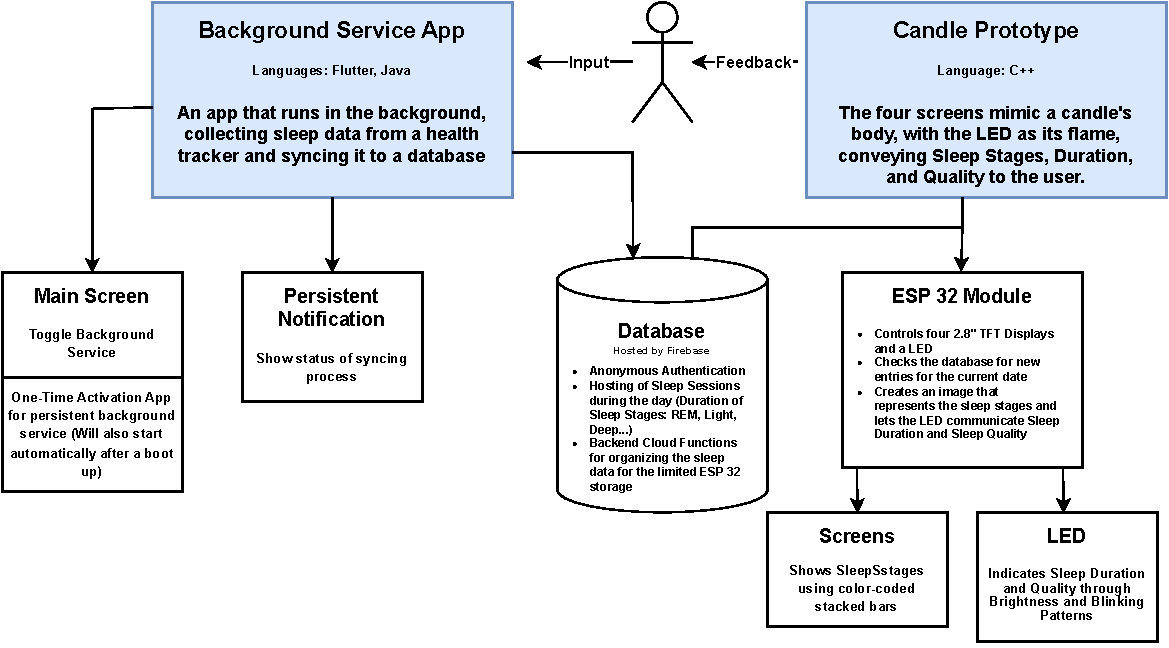
\includegraphics[height=\paperheight, width=\paperwidth, angle=90, keepaspectratio]{graphics/InputOutput.drawio (3).pdf}
    \caption{Implementation and Interaction Layout Diagram}
    \label{fig:inout}
\end{figure}

\chapter{Discussion}

In the previous chapters, we provided a detailed rationale and methodology behind the development of our application and prototype. This final chapter is dedicated to evaluating the results of our prototyping efforts, while acknowledging the limitations of our project and suggesting ways for future research. Previously, we outlined the research process to each of our research questions. We will now outline how our final prototype meets these established criteria, with a particular focus on its usability in sleep environments. This includes a critical examination of how our prototype avoids disturbing the serenity of a calming and relaxing sleep environment.

\section{What categories of sleep data are relevant for effective visualization and understanding?}
Tracking and documenting sleep can be achieved through a variety of metrics, with each user showing a preference for different metrics as each individual experiences sleep in their own unique way. So, to make it easier and more accessible for everyone to track their own sleep health, we have agreed on a global sleep quality score which, together with some other data from the sleep recording, calculates a value between 0 and 100, providing a simple and useful understanding of ones sleep quality. In addition, our prototype is able to communicate other metrics, like sleep duration and sleep stages, which is in alignment with both survey results and is comparable to sleep metrics used in commercial sleep tracking apps.

\section{How should a physical prototype that communicates sleep data look?}
We made the prototype resemble a candle by designing a printed circuit board, which allows for the attachment of 4 TFT screens at each side of the board, ending up with a cubic shape. The ESP32 board is connected at the bottom of the circuit board, leaving enough space in the inside of the cube for the LED's wiring, which is placed on top of the cube. A 3D print aids in visualizing the actual candle, by giving it a stand to also hide the ESP32 board at the bottom, while also offering enough stability to the whole structure. The stand has an opening on the side to leave enough space for a Micro-USB-Standard cable, which powers the whole prototype. The LED's wiring follows through a 3D printed wick, which holds a 3D printed flame-like milky-transparent object, encasing the LED inside of it. By using the ambient design principles inside the tranquil sleep environment, our aim is to help the user find relaxation, by making the communication with the prototype intuitive and effortless. The prototype is around the height of a smartphone with a width not larger than conventional candles. This design meets with the user's concept based on the survey results, offering a calming and relaxing environment.

\section{How should a physical prototype communicate sleep data?}
Our prototype incorporates the sleep data metrics discussed in RQ1, primarily displayed through a gentle light indication that seamlessly integrates into the sleep environment. The LED's flickering is designed to be subtle, mimicking the realistic effect of a candle without emitting disruptive light. When near a wall, this flickering casts shadows, enhancing the candle-like appearance. The LED's brightness and flicker intensity serve not as an alarm but as a gentle reminder: the poorer one's sleep, the more noticeable the light, encouraging mindfulness about sleep habits. When the user observes a pronounced flickering effect, they can engage with the candle directly. By doing so, they can see on the four screens the duration of each sleep stage from the previous night. This feature enables a swift review of potential disruptions, such as instances of waking up.

It should be mentioned, that a vast majority of participants of the online survey asked for a touch-based communication, which would have led to different design and communication choices, as we are now being presented with. Still, we decided to go with light-indicators as our way of communication, since they offer a far more simple implementation into the prototype, compared to a touch-based output, like the manipulation of an object's surface. Also, we assumed that most participants of the online survey were thinking of touchscreens as a form of communication, which would not be a touch-based output.

\section{Limitations and Future Work}
There are some limitations to this project that provide opportunities for further research. In addition to a proper presentation of the data, our survey revealed a number of other factors that hinder motivation to continue using a sleep tracker. Participants who discontinued the use of sleep tracking devices frequently cited discomfort while wearing the devices or the inaccuracy of the recorded data as reasons for stopping. This suggests a path for additional research, focusing on exploring alternative tracking methods to achieve more comfortable and accurate outcomes. Additionally, the survey identified various factors, such as temperature or noise, that impede users from getting quality rest. Although addressing these factors directly may be challenging, a new prototype could be developed to measure certain environmental elements that prevent users from achieving sufficient sleep and inform the user about those factors. 

Our prototype utilizes sleep habits identified in studies as an overall benchmark, allowing for a comparison with the user's own sleep patterns to get a result. Although this method provides a reasonable estimate of a user's sleep health, it may lead to misconceptions for some, as sleep varies greatly among individuals and is influenced by numerous factors such as age, gender, work, hobbies, etc. \cite{patel_physiology_2023}. This variation presents the opportunity for an alternative approach, where an analysis of an user's physical characteristics and daily activities is conducted to establish a personalized benchmark tailored to each individual. Creating a personalized sleep benchmark could also offer users with sleep disorders the opportunity to track their sleep habits without the need to compare them to standard norms, thereby enabling them to make improvements tailored to their specific goals.

The prototype currently has a few limitations, both in software and hardware. It can only display sleep data from the previous night, although survey respondents expressed a preference for viewing data from both the last night and the past week. To address this, an additional Cloud Function could be implemented to gather and average the sleep stage durations from the last seven days, enabling a comprehensive weekly sleep visualization. The prototype's touchscreens could facilitate toggling between nightly and weekly data with a simple gesture. Another challenge is the continuous operation of the screens and LED, which must be manually turned off. A potential solution is to integrate an alarm clock function, allowing the candle to automatically power off when the user goes to bed and gradually reactivates upon waking. The prototype can only display the duration of each sleep stage stacked sequentially, whereas the original intention was to show real-time transitions between sleep stages. From a software perspective, this isn't a major issue, but the limited resolution of the screens (320 pixels in length) restricts the displayable time span to approximately 5.3 hours, assuming each minute of sleep stage is represented by one pixel. To address this, a feasible solution would be to use screens with a higher resolution, such as 720 pixels, which would allow for a 12-hour display. Alternatively, the resolution of the sleep stages could be reduced by only displaying stages that last longer than five minutes. Also, although developed in Flutter, the app is currently only available for Android. This is due to the different approaches required to execute and implement background tasks on different operating systems. iOS, in particular, imposes stricter restrictions and requires a greater focus on integrating native solutions than Android. In terms of setup, the prototype has limitations because it requires manual input of the WiFi SSID and password into the ESP32 board, along with the user's phone device ID. This is necessary because the user's sleep data is stored in a directory named using the device ID. A solution to simplify this process would be to enable Bluetooth connectivity between the ESP32 board and the user's phone. An additional setup feature in the app could then facilitate the transfer of all necessary information to the board via Bluetooth. Furthermore, for establishing a WiFi connection, incorporating a WPS (WiFi Protected Setup) feature could streamline the setup process significantly.

Future research should focus on determining whether users effectively understand the feedback provided by the candle prototype, as well as assessing their reaction to the design. It's also important to conduct user testing of the phone application to identify any compatibility issues with different brands of health trackers. These aspects could be effectively assessed through individual interviews or short term studies.

The primary focus should be to conduct a long-term study to verify the accuracy of the assumptions made during the development of the system, using the results of the study and existing research. In particular, this study should assess whether the visualization of sleep data in the system helps users to understand and potentially improve their sleep habits. In addition, to determine the effectiveness of the prototype's ambient design, a comparison of the system with a control group using medical-grade sleep tracking devices would be crucial.


\chapter{Conclusion}
In our study, we created a physical object based on the principles of ambient design. This object aims to address the difficulty of understanding personal sleep health. This is done by transforming the interpretation of collected sleep data into a more intuitive and accessible form. Our review of various sleep tracking studies revealed numerous challenges and opportunities in the field of sleep monitoring. \cite{Challenges_Oppotunieties_SleepTracking}. Common problems include a lack of understanding of sleep data, as commercial sleep tracking applications present this data primarily in the form of graphs and scores. While these can provide detailed insights into sleep patterns, they don't explicitly indicate whether one's sleep habits are healthy without further personal research. In addition, a significant challenge is the time required to thoroughly understand the complex nature of sleep data and sessions, which is essential to identify and implement beneficial changes to improve sleep health. To address these concerns, we aimed to present users' sleep data in a visually intuitive physical form that seamlessly integrates into the typical sleep environment.

Our research primarily focused on the abstract concept of sleep health. To make this concept more tangible, we created a prototype designed to enhance users' connection with their sleep habits and stimulate greater interest in their sleep health. This prototype, inspired by various design directions identified in our research, is crafted to blend smoothly into a person's bedroom. It aims to offer a peaceful visualization of sleep patterns without interfering with daily activities.

Our research required a deeper exploration of how the theory of a physical sleep data representation could be applied in practice. To inform our design, we developed survey questions based on these theoretical concepts. The results showed that a significant number of people had never used a health tracker, and many of those who did eventually stopped using it. The main reasons for this were discomfort and simply forgetting to use the device. For those who did use sleep tracking devices, there was no noticeable improvement in sleep habits, often due to a lack of motivation to change them. To refine our understanding of the prototype design, we decided to conduct a focus group. The purpose of this additional step was to gather different ideas and perspectives to help us build a solid foundation for the development of our prototype. These findings gave us a clearer understanding of the limitations of current sleep tracking devices and highlighted potential ways to effectively visualize sleep data.

In response to the survey results, we came up with  a candle-like design that visually represents sleep quality, duration and the length of different sleep stages. This candle mimics the natural behavior of a real flame, using characteristics such as brightness and flicker to communicate sleep data in an intuitive and non-intrusive way. If users notice any anomalies in their sleep quality as represented by the candle, they can examine its body, which consists of four screens arranged in a cube. These screens use stacked colored bars to indicate the duration of different stages of sleep.

Our research participants expressed a strong preference for a smartphone-sized, interactive object that could be placed next to the bed. We chose light-indication for our design because of its simplicity of implementation. This decision was also influenced by the fact that every prototype developed in our focus group used some form of visual data representation. 

Our prototype will serve as the basis for future research in this area. The next stage is to test our findings in real sleep environments and to refine the prototype. Future research should then focus on improving the tracking experience, making it more comfortable, and integrating this improved tracking with a more intuitive data presentation. This approach should be evaluated in a long-term study to fully assess its effectiveness.

This paper represents a first step into exploring alternative ways of representing sleep habits using ambient design principles, and investigating their potential to enhance these habits in our fast-paced, technology-centric world. Through continued research, we hope to make a significant contribution to the understanding of sleep habits and ultimately facilitate meaningful improvements in overall sleep health, mental health and physical well-being.

\printbibliography

All links were last followed on \today.

\appendix

\chapter{Appendix}
\label{appendix:appendix_A}
\begin{figure}[H]
    \centering
    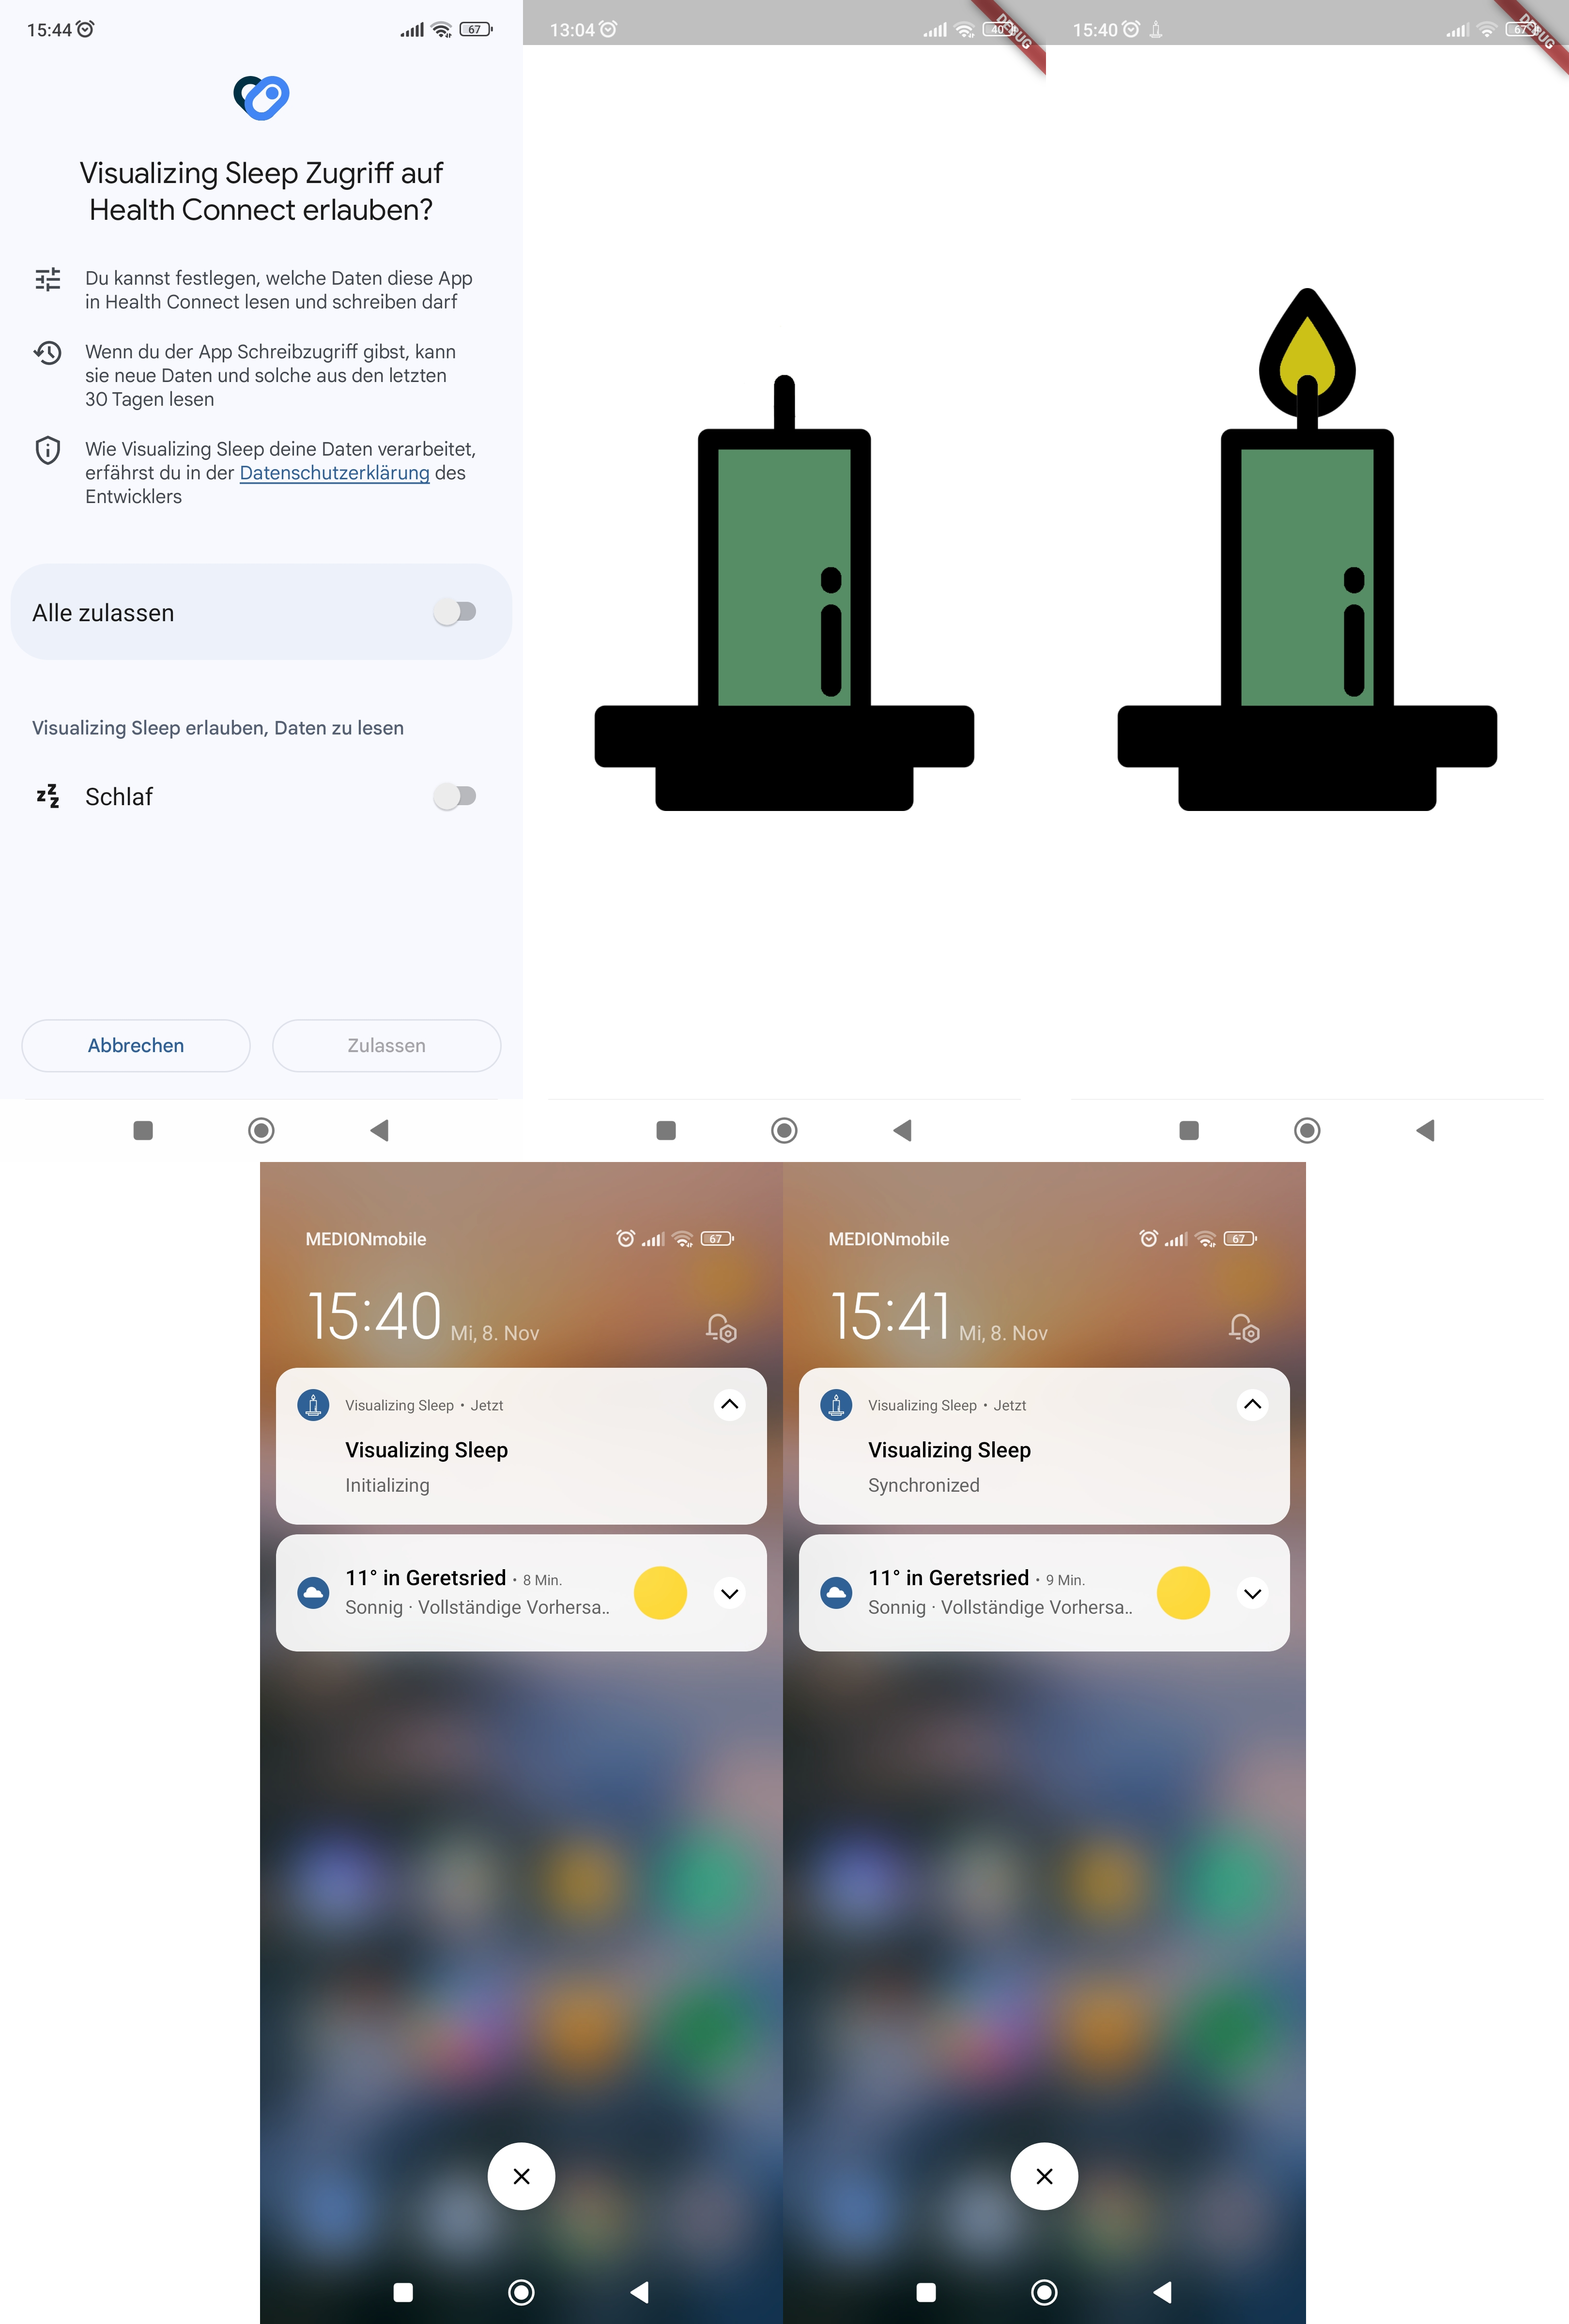
\includegraphics[scale=0.50]{graphics/SetupVis.png}
    \caption{Setting up the App}
    \label{fig:App-Setup}
\end{figure}

\begin{figure}[H]
    \centering
    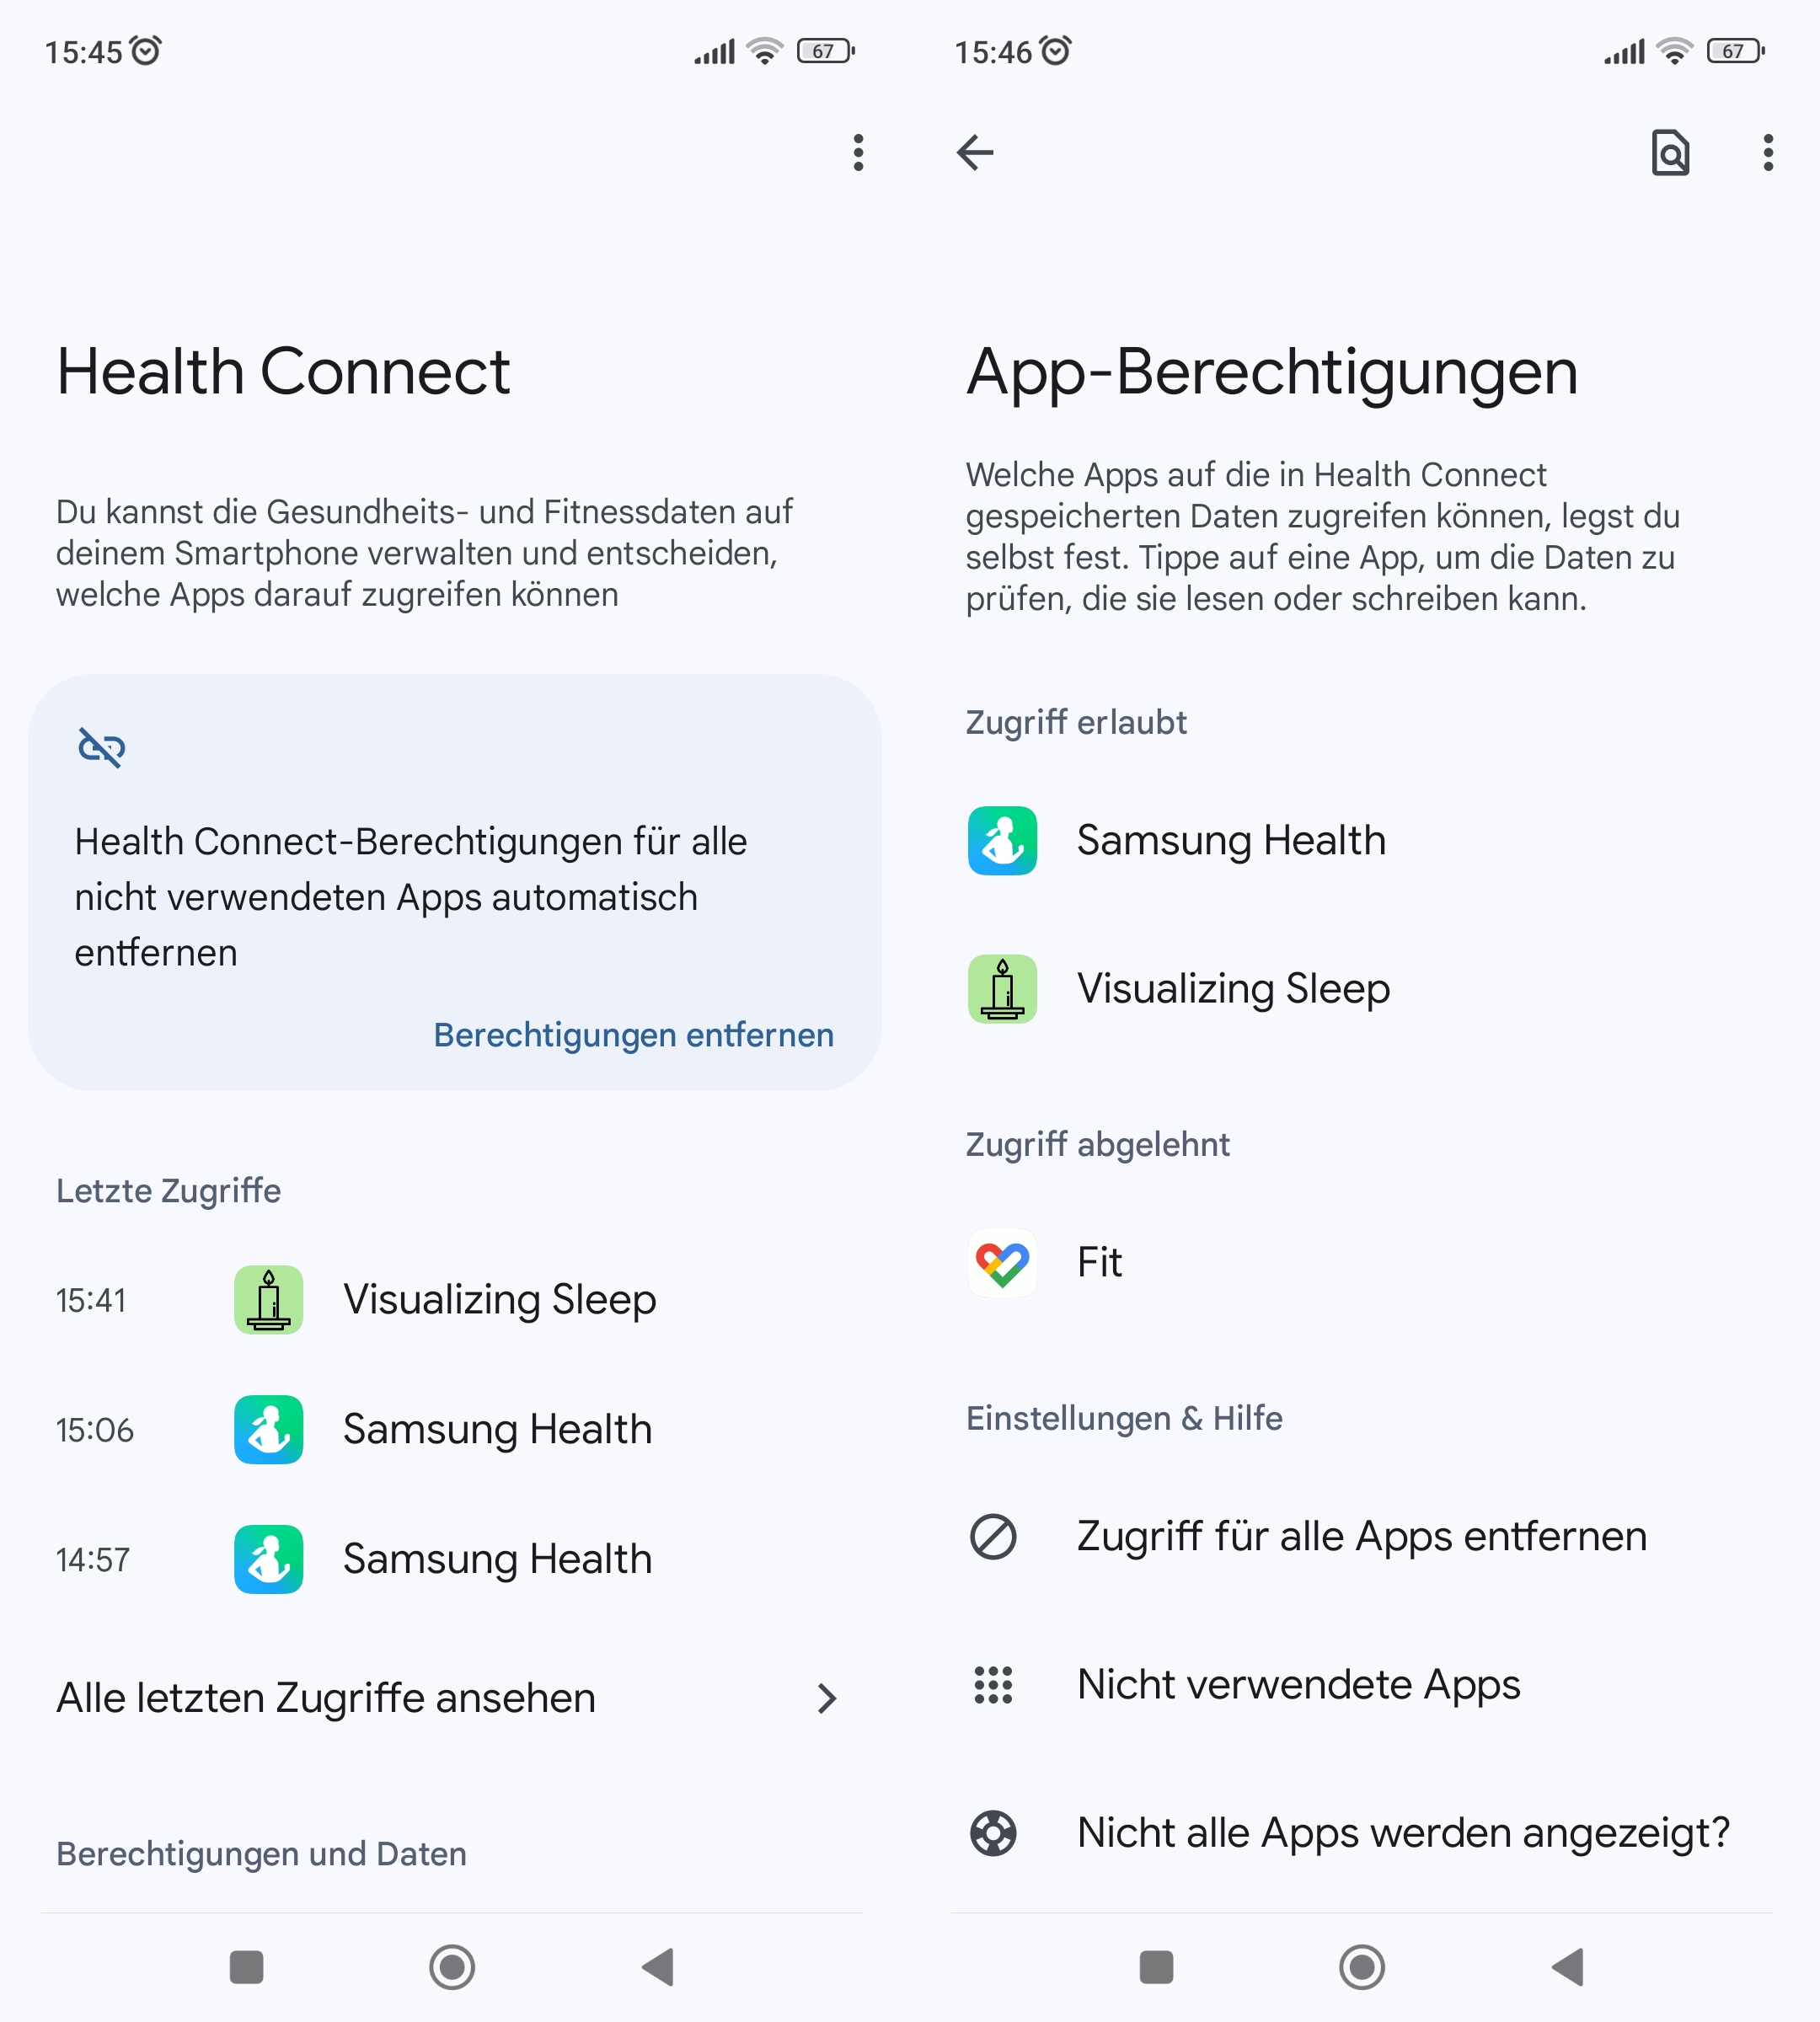
\includegraphics[scale=0.6]{graphics/HealthConnectStartRights.png}
    \caption{Giving Access to Health Apps}
    \label{fig:HealthApp-Access}
\end{figure}

\begin{figure}[H]
    \centering
    \includegraphics[scale=0.2]{graphics/Prototyping.png}
    \caption{Prototype v1}
    \label{fig:Prototype_v1}
\end{figure}

\begin{figure}[H]
    \centering
    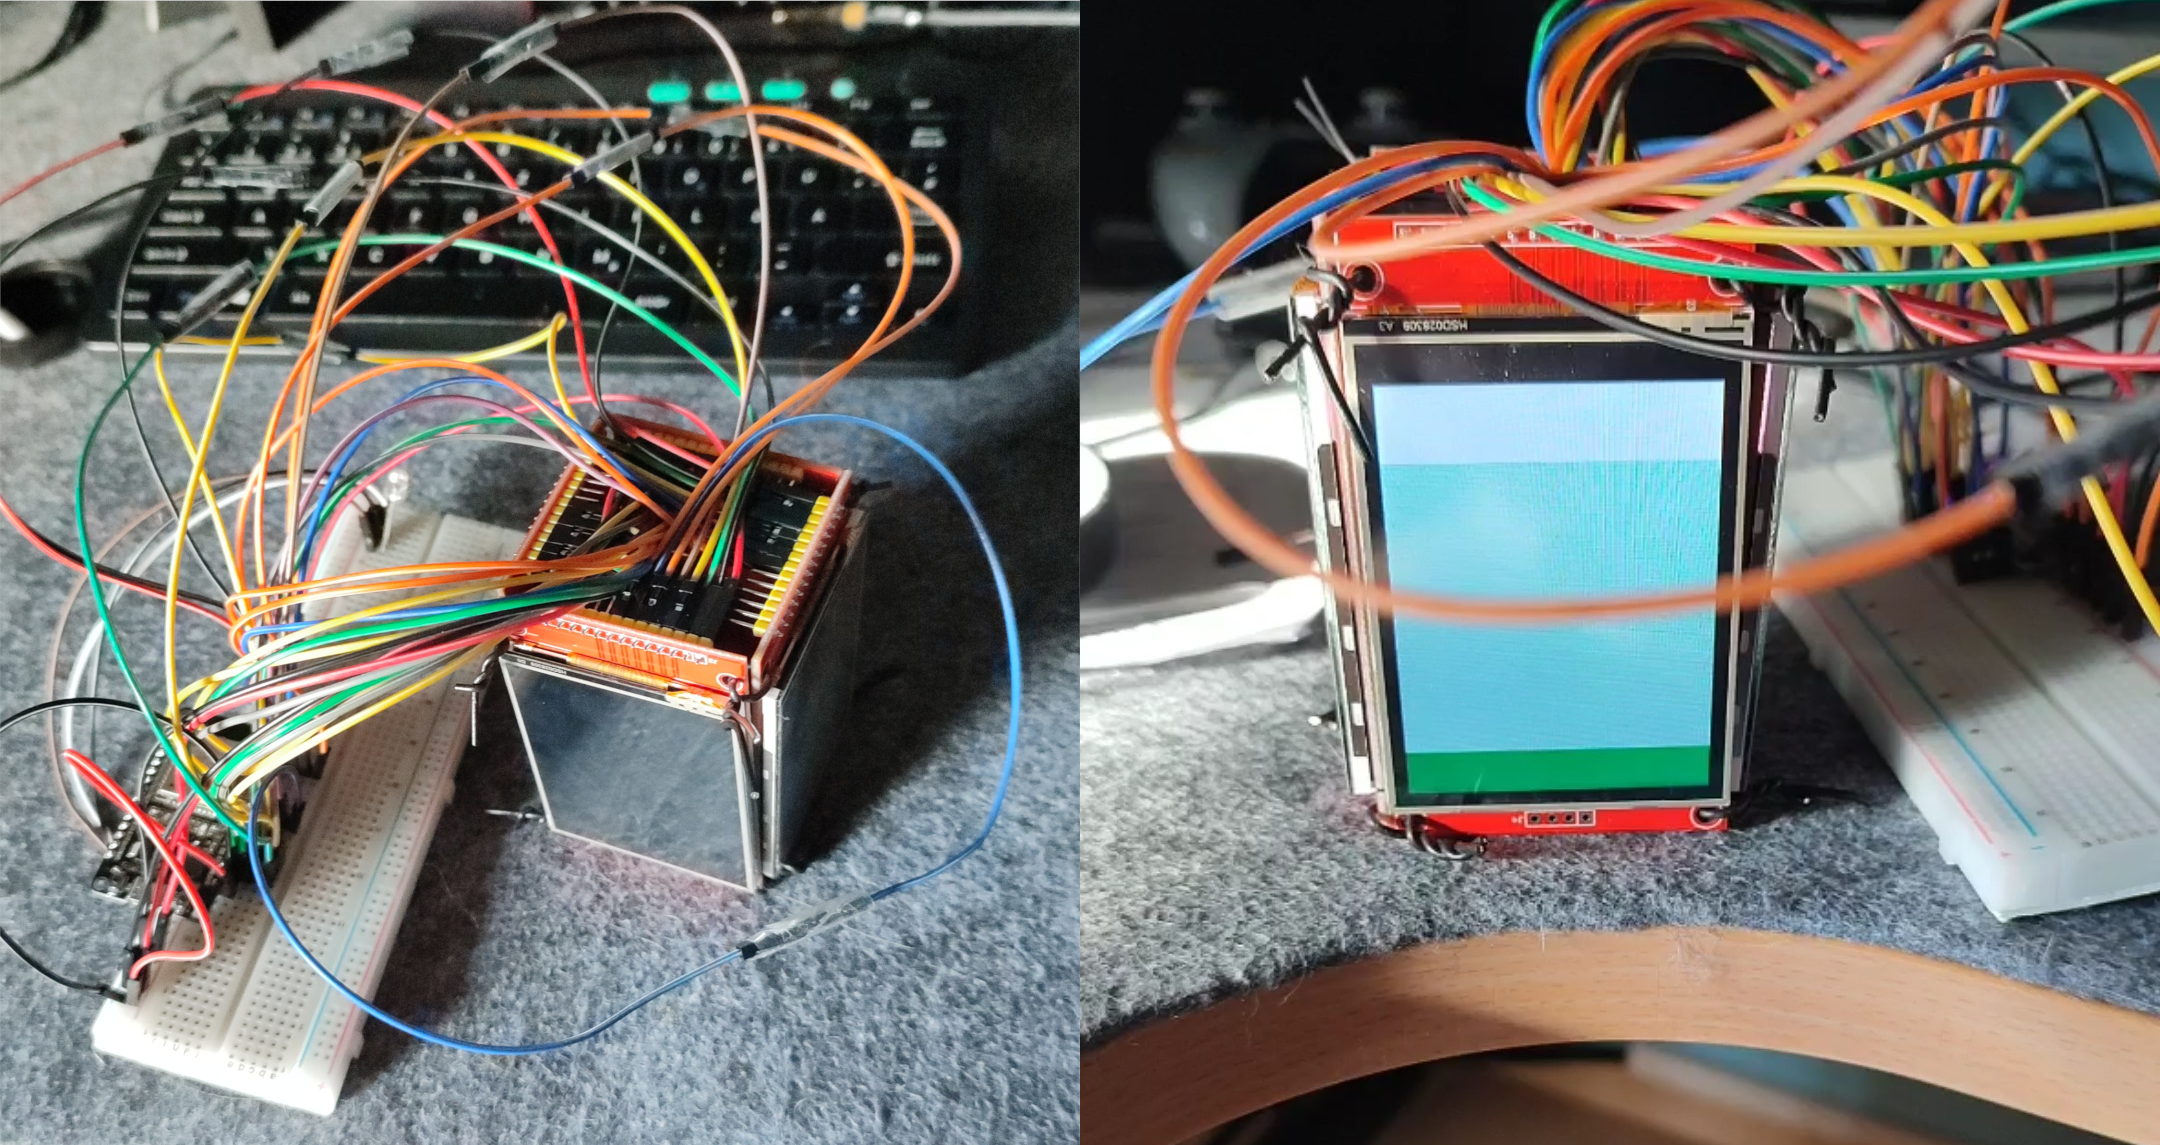
\includegraphics[scale=0.7]{graphics/Prototype2.png}
    \caption{Prototype v2}
    \label{fig:Prototype_v2}
\end{figure}

\begin{figure}[H]
    \centering
    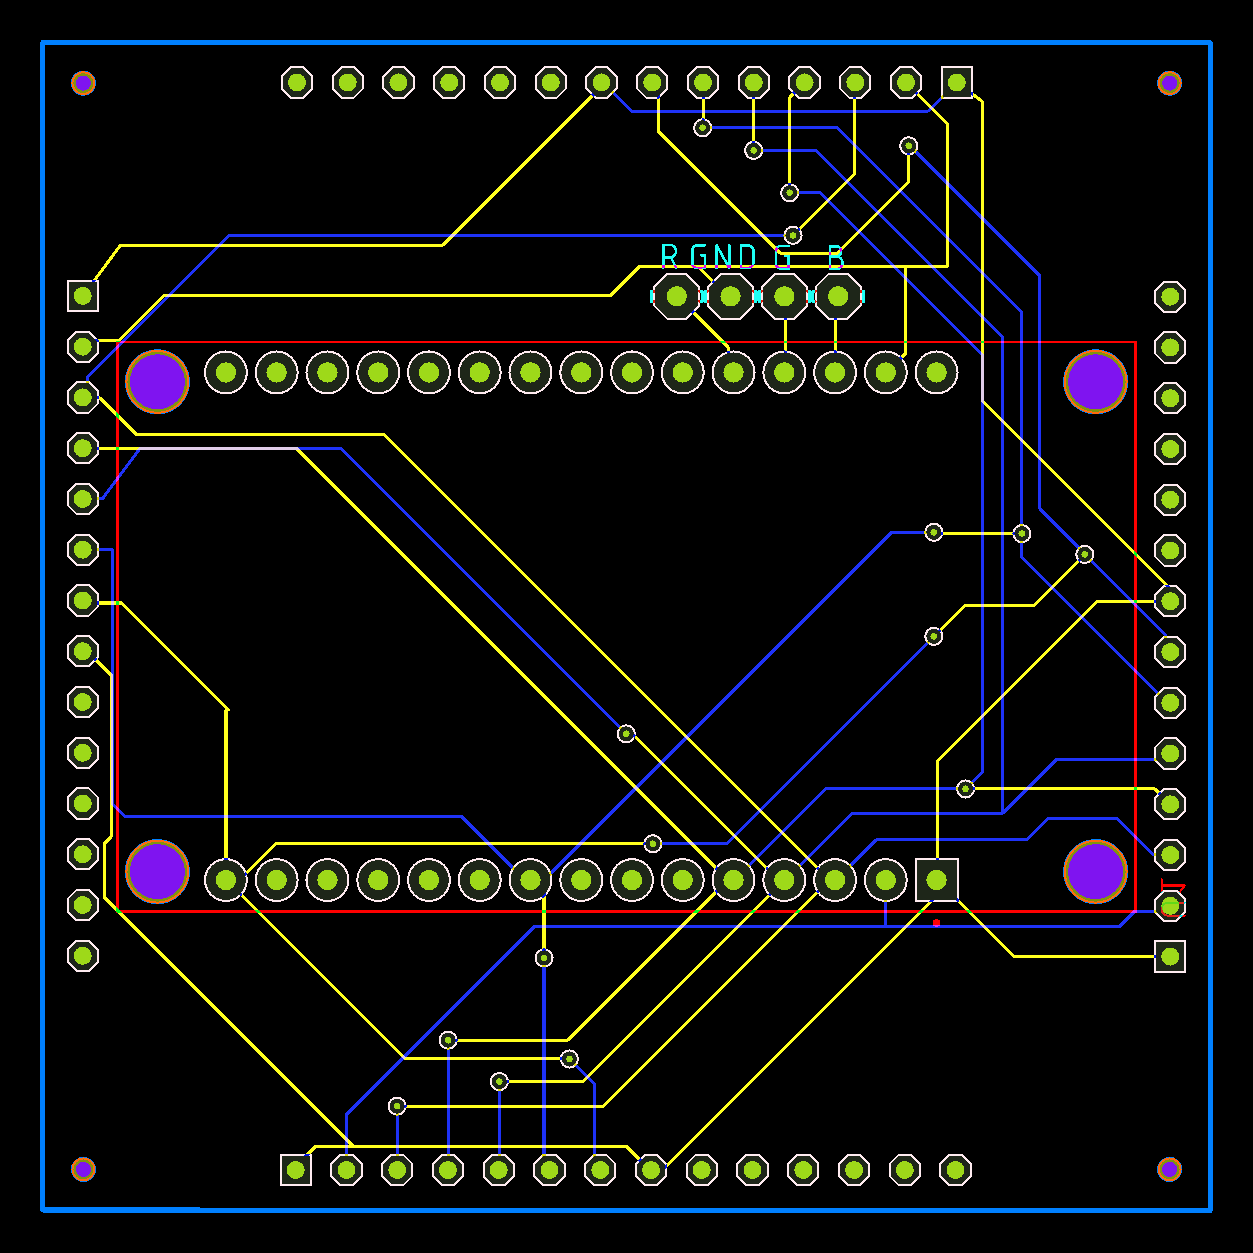
\includegraphics[scale=0.3]{graphics/PCB.png}
    \caption{Circuit Board Scheme}
    \label{fig:PCB}
\end{figure}

\begin{figure}
    \centering
    \includegraphics[scale=0.25]{graphics/FocusGroupAppendix.png}
    \caption{Focus Group Sketches}
    \label{fig:Focus_Group_Sketches}
\end{figure}

\chapter{Appendix}
\label{appendix:appendix_B}
\text{Variables having an apostrophe at the end resemble the considered healthy benchmark value.}
\begin{equation}
    \centering
    \textbf{s} = w_{1}\cdot\left | light{}' - light \right | + w_{2}\cdot\left | deep{}' - deep \right | + w_{3}\cdot\left | rem{}' - rem \right |
\end{equation}
\text{where $\textbf{s}$ is the sleep stages change, $w_{1}, w_{2}, w_{3}$ are weights, and $light, deep, rem$ are sleep phases.}
\begin{equation}
    \centering
    \textbf{e} = \left | efficiency{}' - efficiency \right |
\end{equation}
\text{where $\textbf{e}$ is the efficiency change, and $efficiency$ is the initial sleep efficiency.}
\begin{equation}
    \centering
    \textbf{a} = \left | awakenings{}' - awakenings \right |
\end{equation}
\text{where $\textbf{a}$ measures the change in the number of awakenings.}
\begin{equation}
    \centering
    \textbf{d} = \left | duration{}' - duration \right |
\end{equation}
\text{where $\textbf{d}$ is the change in sleep duration.}
\begin{equation}
    \textbf{Sleep Quality} = 100 - \max(0, \min(v_{1} \cdot \textbf{s}
    + v_{2} \cdot \textbf{e}
    + v_{3} \cdot \textbf{a}
    + v_{4} \cdot \textbf{d}), 100)
\end{equation}
\text{with $v_{1}, v_{2}, v_{3}, v_{4}$ as the respective weights.}
%% !TeX root = main-english.tex
% !TeX spellcheck = en-US
% !TeX encoding = utf8
% -*- coding:utf-8 mod:LaTeX -*-

%This smart spell only works if no changes have been made to the chapter 
%using the options proposed in preambel/chapterheads.tex.
\setchapterpreamble[u]{%
  \dictum[Albert Einstein]{We cannot solve our problems with the same level of thinking that created them}
}
\chapter{LaTeX Hints}
\label{chap:latexhints}

One sentence per line.
This rule is important for the usage of version control systems.
A new line is generated with a blank line.
As you would do in Word:
New paragraphs are generated by pressing enter.
In LaTeX, this does not lead to a new paragraph as LaTeX joins subsequent lines.
In case you want a new paragraph, just press enter twice (!).
This leads to an empty line.
In word, there is the functionality to press shift and enter.
This leads to a hard line break.
The text starts at the beginning of a new line.
In LaTeX, you can do that by using two backslashes (\textbackslash\textbackslash).
This is rarely used.

Please do \textit{not} use two backslahes for new paragraphs.
For instance, this sentence belongs to the same paragraph, whereas the last one started a new one.
A long motivation for that is provided at \url{http://loopspace.mathforge.org/HowDidIDoThat/TeX/VCS/#section.3}.

One can write \emph{emphasized text (rendered in italics)} and \textbf{bold text}.

\section{File Encoding and Support of Umlauts}
\label{sec:firstsectioninlatexhints}
The template offers foll UTF-8 support.
All recent editors should not have issues with that.

\section{Citations}


References are set by means of \texttt{\textbackslash cite[key]}.

\begin{filecontents*}{\democodefile}
Example: \cite{WSPA} or by author input: \citet{WSPA}.
\end{filecontents*}
\PrintDemo{style=parallel}

The following sentence demonstrates
\begin{inparaenum}[1.]
  \item the capitalization of author names at the beginning of the sentence,
  \item the correct citation using author names and the reference,
  \item that the author names are a hyperlink to the bibliography and that
  \item the bibliography contains the name prefix \qq{van der} of \qq{Wil M.\,P.\ van der Aalst}.
\end{inparaenum}

\begin{filecontents*}{\democodefile}
\Citet{RVvdA2016} present a study on the effectiveness of workflow management systems.
\end{filecontents*}
\PrintDemo{style=parallel}

The following sentence demonstrates that you can overwrite the text part of the generated label using \texttt{label} in a bibliopgrahie"=entry, but the year and the uniqueness is still generated by biber.

\begin{filecontents*}{\democodefile}
The workflow engine Apache ODE \cite{ApacheODE} executes \BPEL processes reliably.
\end{filecontents*}
\PrintDemo{style=parallel}

\begin{filecontents*}{\democodefile}
Words are best enclosed using \texttt{\textbackslash qq\{..\}}, then the correct quotes are used.
\end{filecontents*}
\PrintDemo{style=parallel}

When creating the Bibtex file it is recommended to make sure that the DOI is listed.

\section{Formulas and Equations}
\label{sec:mf}

\begin{filecontents*}{\democodefile}
Equations $f(x)=x$ inside the text can be provided.
\end{filecontents*}
\PrintDemo{style=parallel}

A list with all available mathematical symbols is provided at \url{http://texdoc.net/pkg/symbols-a4}.

\begin{filecontents*}{\democodefile}
As example the set of natural numbers is given by $\mathbb{N}$.
\end{filecontents*}
\PrintDemo{style=parallel}

For the documentation of editing mathematical formulas read the package documentation of \texttt{amsmath}\footnote{\url{http://texdoc.net/pkg/amsmath}}.

Equation~\ref{eq:test} is numbered and can be referenced in the text:
\begin{filecontents*}{\democodefile}
\begin{align}
  \label{eq:test}
  x = y
\end{align}
\end{filecontents*}
\PrintDemo{style=parallel}

Following equation is not numbered because of using \texttt{\textbackslash align*} as environment.
\begin{filecontents*}{\democodefile}
\begin{align*}
  x = y
\end{align*}
\end{filecontents*}
\PrintDemo{style=parallel}

The template offers \verb+\abs+ to enable the bars scaling well at the absolute value:

\begin{filecontents*}{\democodefile}
$\abs{X}$.
\end{filecontents*}
\PrintDemo{style=parallel}

More details about mathematical environments provides the documentation available at \url{http://www.ctan.org/tex-archive/help/Catalogue/entries/voss-mathmode.html}.


%%%%%%%%%%%%%%%%%%%%%%%%%%%%%%%%%%%%%%%%%%%%%%%%%%%%%%%%%%%%%%%%%%%%%%%%%%%%%%
\section{Sourcecode}
%%%%%%%%%%%%%%%%%%%%%%%%%%%%%%%%%%%%%%%%%%%%%%%%%%%%%%%%%%%%%%%%%%%%%%%%%%%%%%
\autoref{lst:ListingANDlstlisting} shows how to emmbed source code.
With \texttt{\textbackslash lstinputlisting} the source code can be loaded directly from files.

%Listing-Umgebung wurde durch \newfloat{Listing} definiert
\begin{Listing}
  \begin{lstlisting}
<listing name="second sample">
  <content>not interesting</content>
</listing>
\end{lstlisting}
  \caption{The code is separated by two horizontal lines in the listings environment.}
  \label{lst:ListingANDlstlisting}
\end{Listing}

\begin{filecontents*}{\democodefile}
Source code is also available in the text \lstinline|<listing />|.
\end{filecontents*}
\PrintDemo{style=parallel}


%%%%%%%%%%%%%%%%%%%%%%%%%%%%%%%%%%%%%%%%%%%%%%%%%%%%%%%%%%%%%%%%%%%%%%%%%%%%%%
\section{Pseudocode}
%%%%%%%%%%%%%%%%%%%%%%%%%%%%%%%%%%%%%%%%%%%%%%%%%%%%%%%%%%%%%%%%%%%%%%%%%%%%%%
\autoref{alg:sample} shows a sample algorithm.
\begin{Algorithmus} %Use the environment only if you want to place the algorithm similar to graphics from TeX
  \caption{Sample algorithm}
  \label{alg:sample}
  \begin{algorithmic}
\Procedure{Sample}{$a$,$v_e$}
\State $\mathsf{parentHandled} \gets (a = \mathsf{process}) \lor \mathsf{visited}(a'), (a',c,a) \in \mathsf{HR}$
\State \Comment $(a',c'a) \in \mathsf{HR}$ denotes that $a'$ is the parent of $a$
\If{$\mathsf{parentHandled}\,\land(\mathcal{L}_\mathit{in}(a)=\emptyset\,\lor\,\forall l \in \mathcal{L}_\mathit{in}(a): \mathsf{visited}(l))$}
\State $\mathsf{visited}(a) \gets \text{true}$
\State $\mathsf{writes}_\circ(a,v_e) \gets
\begin{cases}
\mathsf{joinLinks}(a,v_e) & \abs{\mathcal{L}_\mathit{in}(a)} > 0\\
\mathsf{writes}_\circ(p,v_e)
& \exists p: (p,c,a) \in \mathsf{HR}\\
(\emptyset, \emptyset, \emptyset, false) & \text{otherwise}
\end{cases}
$
\If{$a\in\mathcal{A}_\mathit{basic}$}
  \State \Call{HandleBasicActivity}{$a$,$v_e$}
\ElsIf{$a\in\mathcal{A}_\mathit{flow}$}
  \State \Call{HandleFlow}{$a$,$v_e$}
\ElsIf{$a = \mathsf{process}$} \Comment Directly handle the contained activity
  \State \Call{HandleActivity}{$a'$,$v_e$}, $(a,\bot,a') \in \mathsf{HR}$
  \State $\mathsf{writes}_\bullet(a) \gets \mathsf{writes}_\bullet(a')$
\EndIf
\ForAll{$l \in \mathcal{L}_\mathit{out}(a)$}
  \State \Call{HandleLink}{$l$,$v_e$}
\EndFor
\EndIf
\EndProcedure
  \end{algorithmic}
\end{Algorithmus}

\clearpage
And if you want to write an algorithm that goes over several pages, you can only do this with the following \textbf{dirty} hack:

{
\begin{minipage}{\textwidth}
  \hrule height .8pt width\textwidth
  \vskip.3em%\vskip\abovecaptionskip\relax
  \stepcounter{Algorithmus}
  \addcontentsline{alg}{Algorithmus}{\protect\numberline{\theAlgorithmus}{\ignorespaces Description \relax}}
  \noindent\textbf{Algorithmus \theAlgorithmus} Description
  %\stepcounter{algorithm}
  %\addcontentsline{alg}{Algorithmus}{\thealgorithm{}\hskip0em Description}
  %\textbf{Algorithmus \thealgorithm} Description
  \vskip.3em%\vskip\belowcaptionskip\relax
  \hrule height .5pt width\textwidth
\end{minipage}
%without the following line, the text is nerer at the rule
\vskip-.3em
%
code goes here\\
test2\\
%
\vskip-.7em
\hrule height .5pt width\textwidth
}


%%%%%%%%%%%%%%%%%%%%%%%%%%%%%%%%%%%%%%%%%%%%%%%%%%%%%%%%%%%%%%%%%%%%%%%%%%%%%%
\section{Figures}
%%%%%%%%%%%%%%%%%%%%%%%%%%%%%%%%%%%%%%%%%%%%%%%%%%%%%%%%%%%%%%%%%%%%%%%%%%%%%%
The \autoref{fig:chor1} and \ref{fig:chor2} are important to understand this document.
In the appendix \vref{fig:AnhangsChor} shows again the complete choreography.

%The parameters in square brackets are optional - e.g. [htb!]
%htb! means: Dear LaTeX, please place this image here first ("_h_ere"). If this does not work, place it at the "_t_op" of the page. And if this is not possible, please place it at the "_b_ottom" of the page. And please, please prefer here and above, even if it doesn't look so optimal ("!")
%These should NOT be used if possible. LaTeX's algorithm for placing the glide environment is already very good!
\begin{figure}
  \centering
  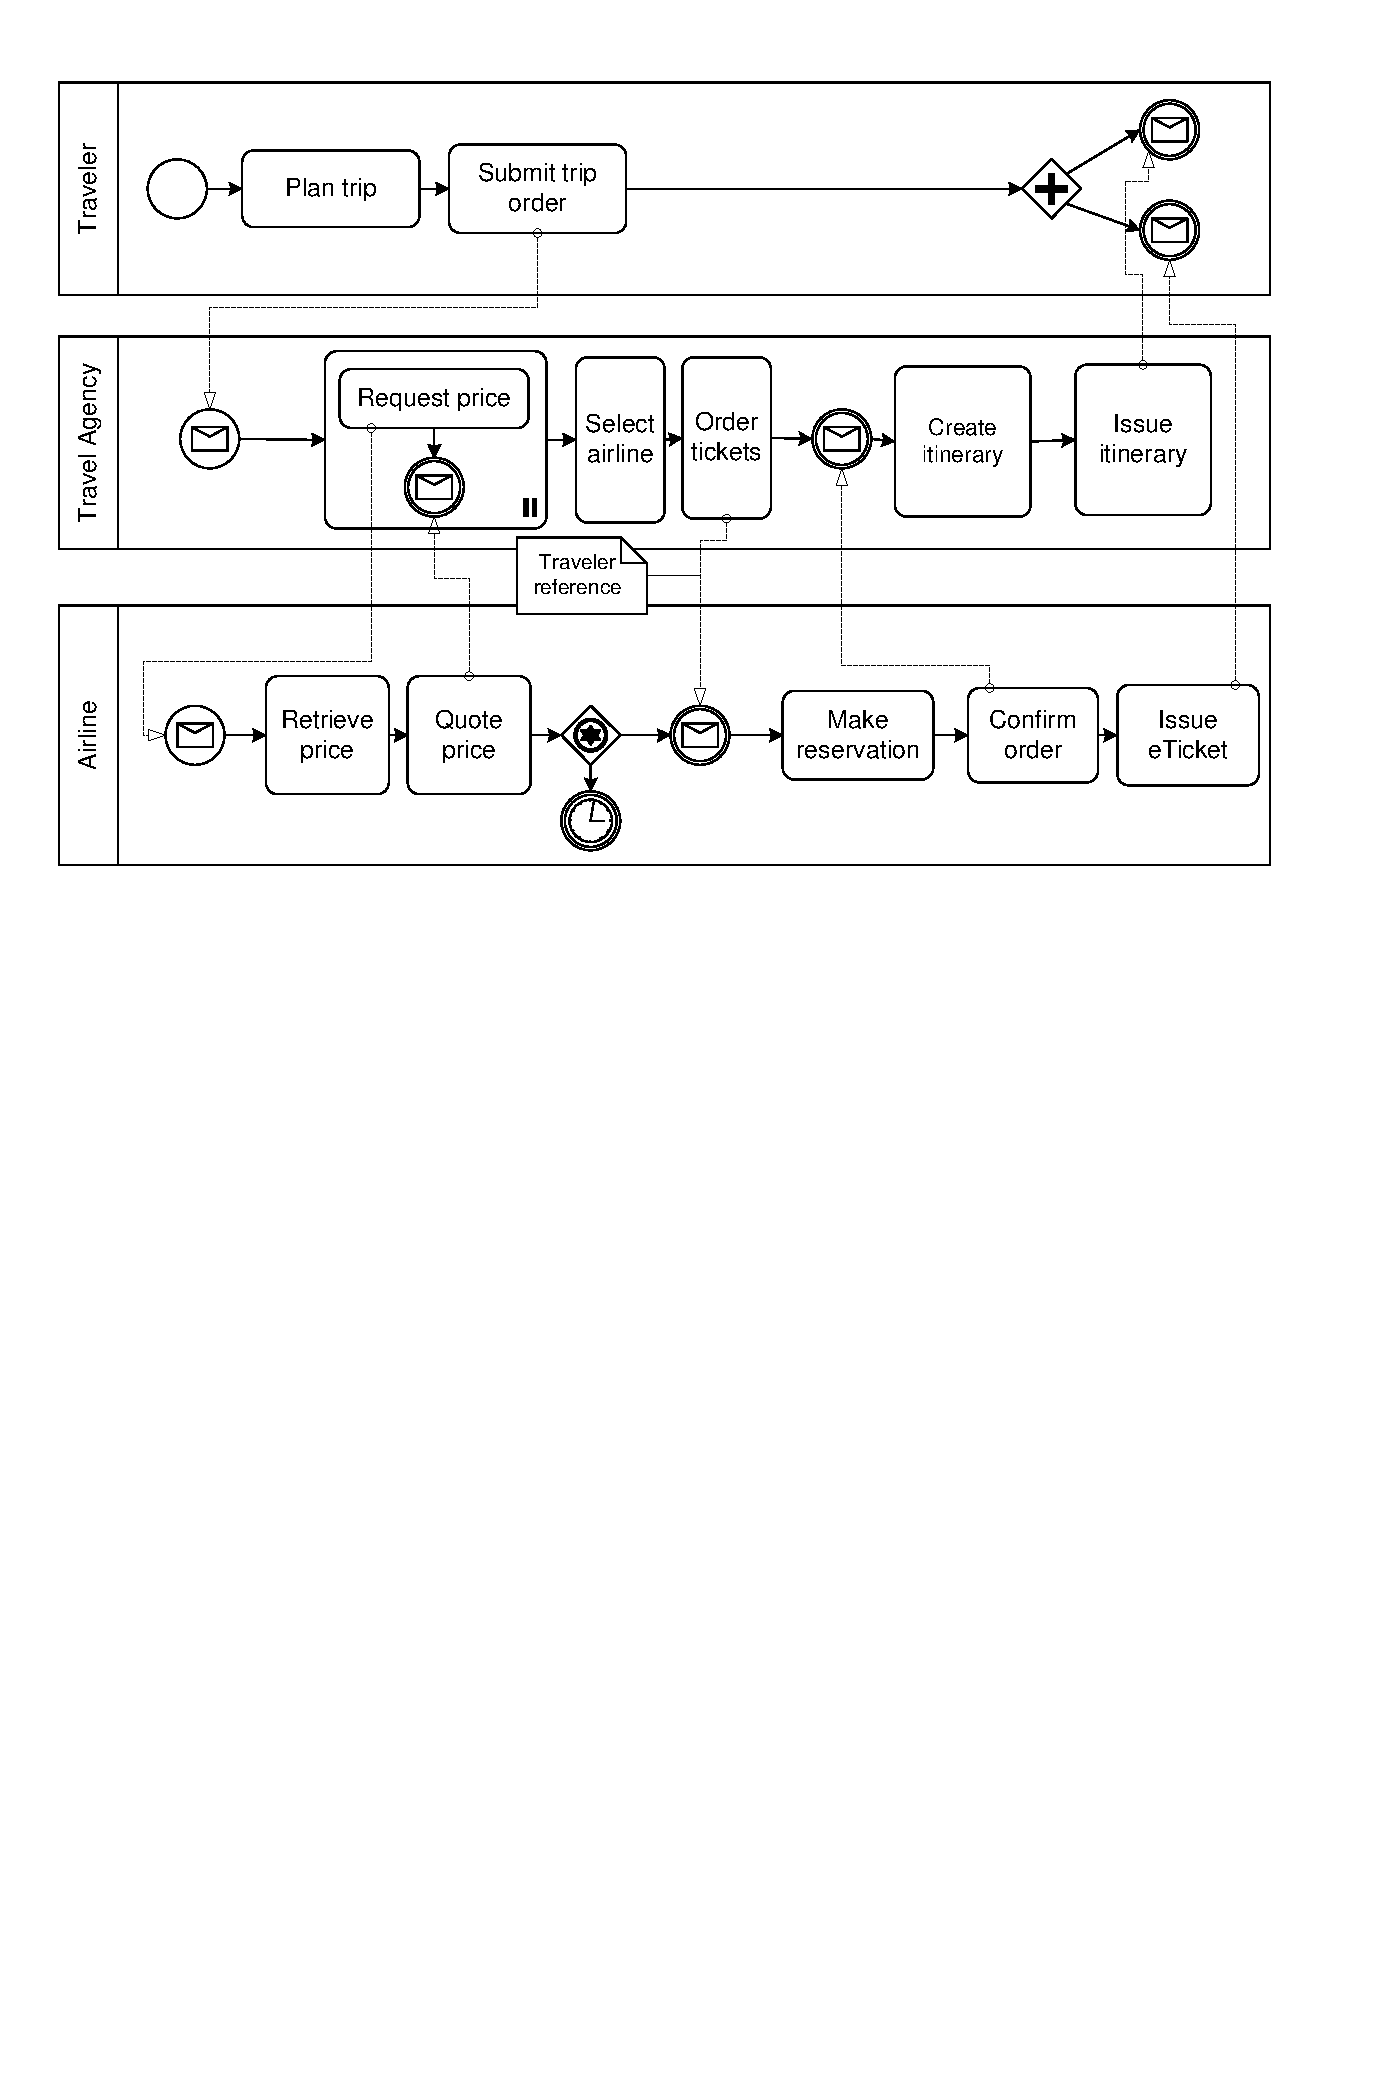
\includegraphics[width=\textwidth]{choreography.pdf}
  \caption{Example Choreography}
  \label{fig:chor1}
\end{figure}

\begin{figure}
  \centering
  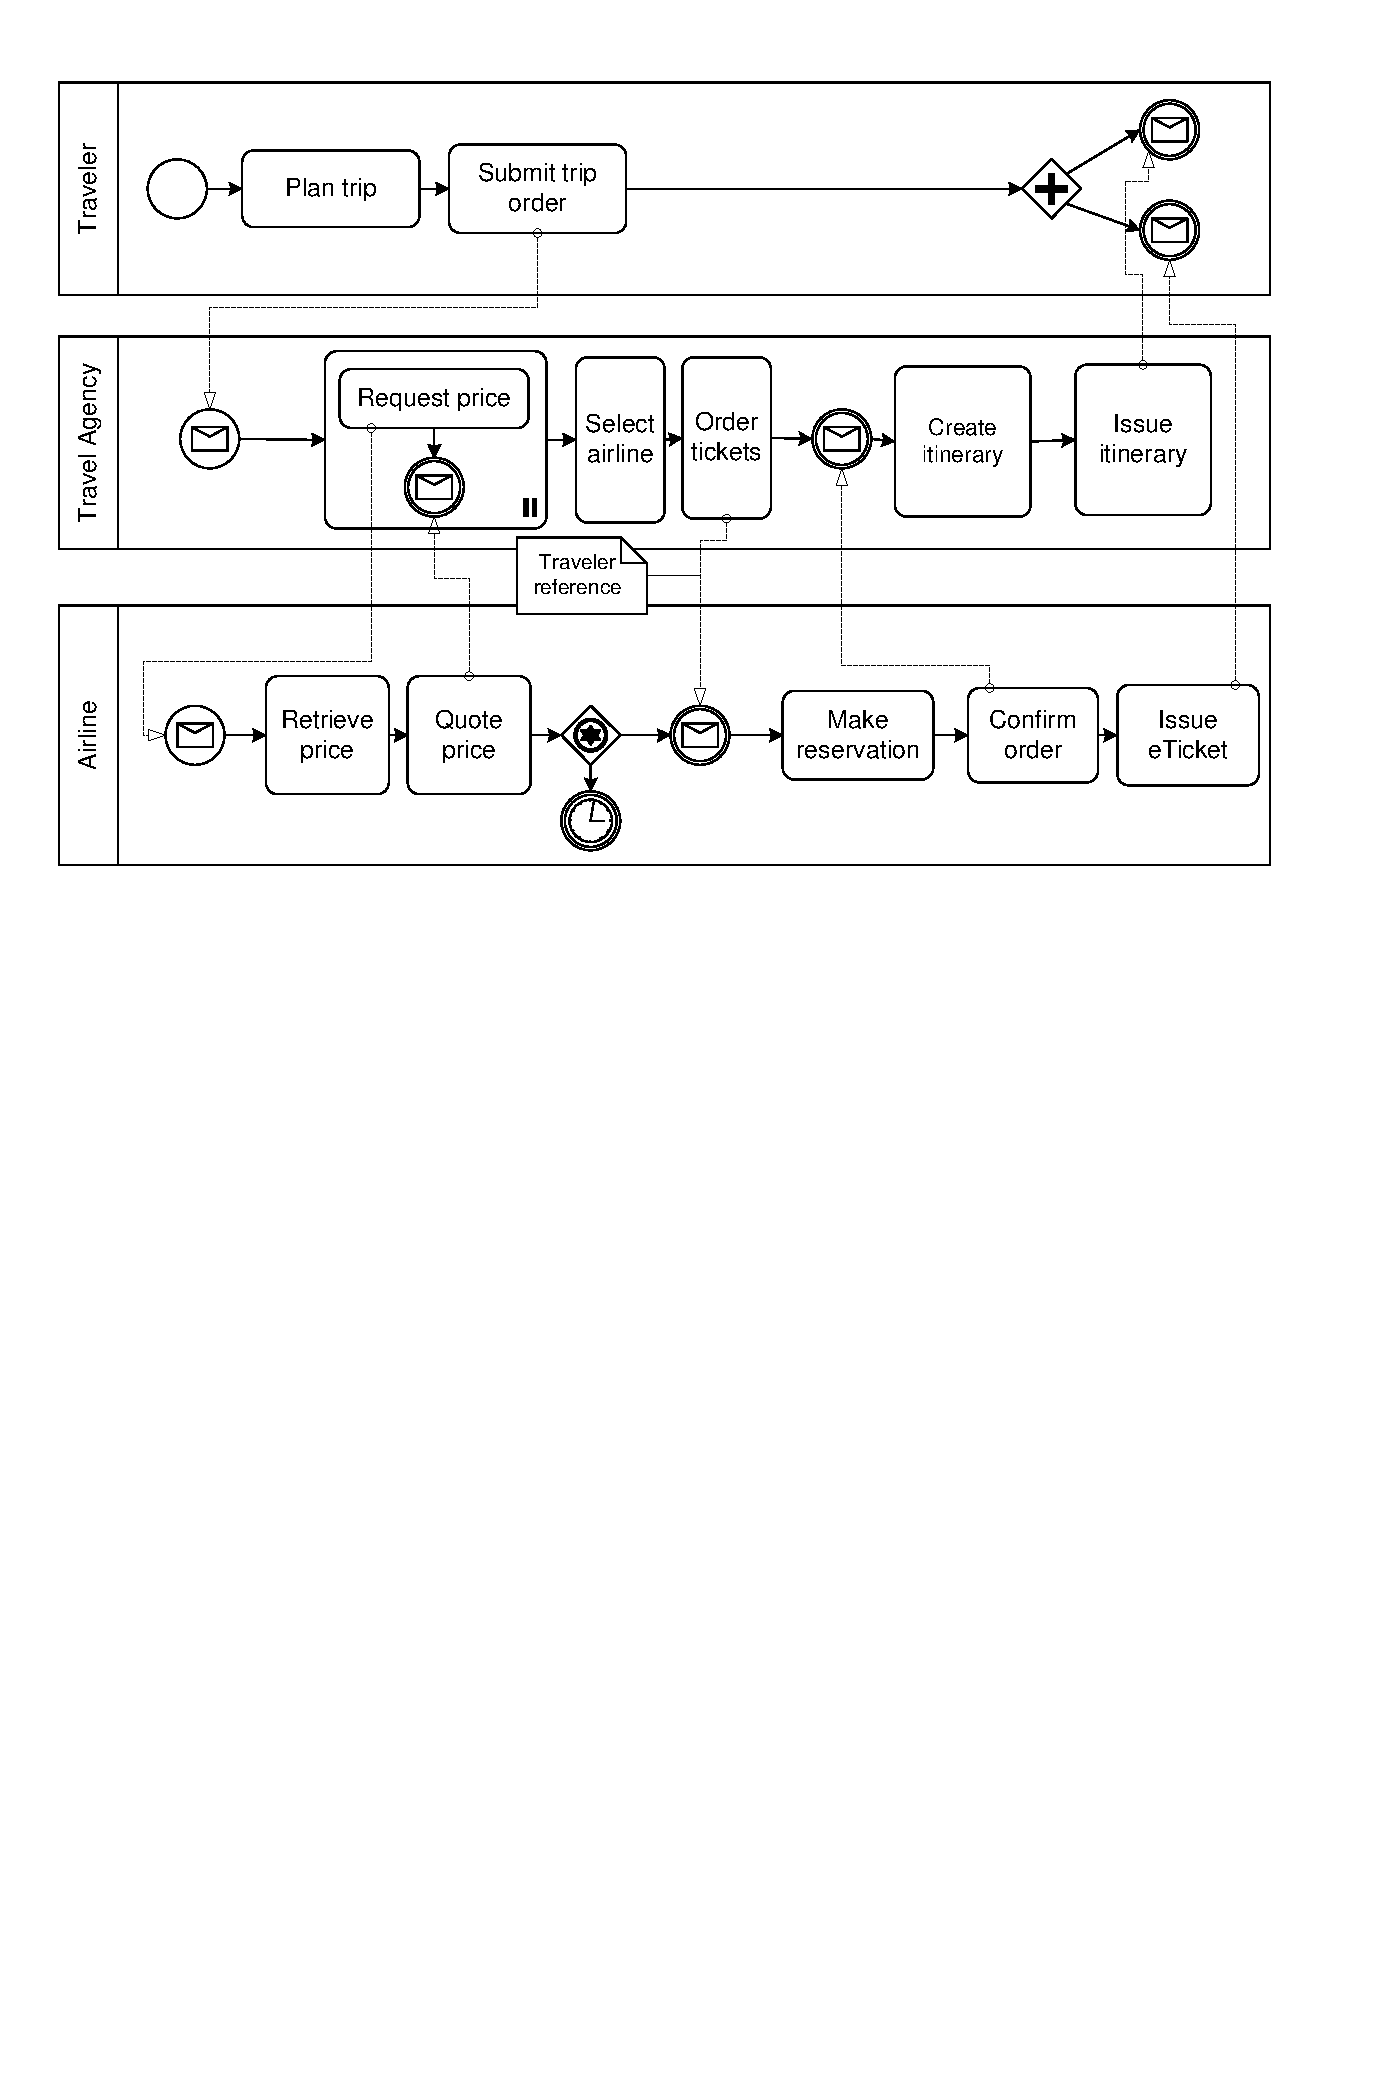
\includegraphics[width=.8\textwidth]{choreography.pdf}
  \caption[Example Choreography]{The example choreography. Now slightly smaller to demonstrate \texttt{\textbackslash textwidth}. And also the use of alternative captions for the list of images. However, the latter is only conditionally recommended, because who reads so much text under a picture? Or is it just a matter of style?}
  \label{fig:chor2}
\end{figure}


\begin{figure}
  \hfill
  \begin{subfigure}{.3\textwidth}
    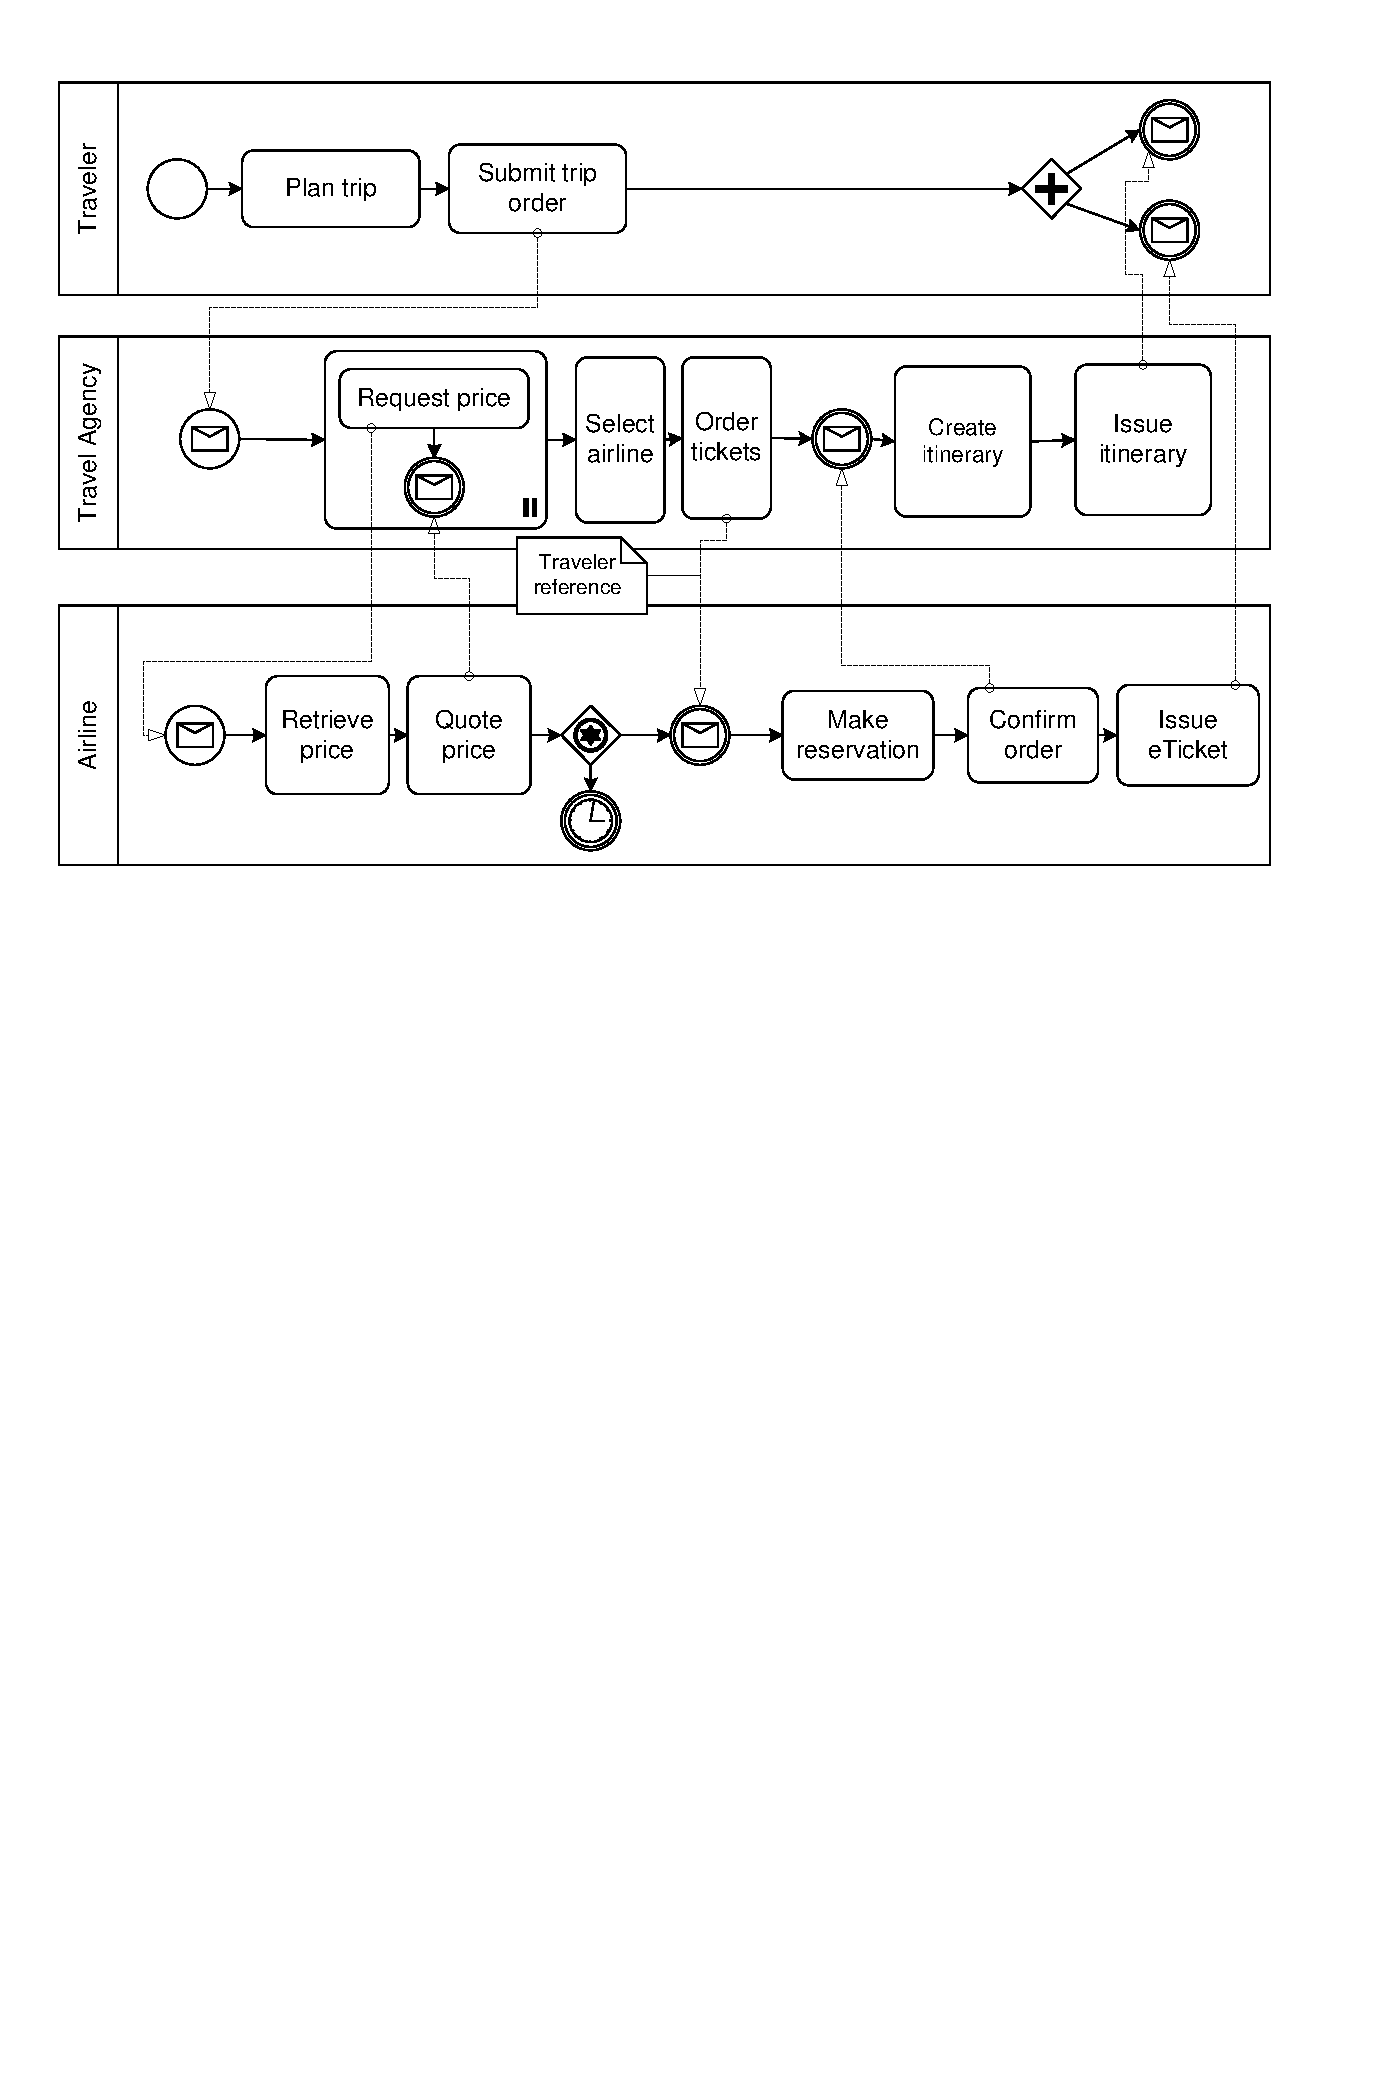
\includegraphics[width=\textwidth]{choreography.pdf}
    \caption{Choreography 1}
    \label{fig:subfigA}
  \end{subfigure}
  \hfill
  \begin{subfigure}{.3\textwidth}
    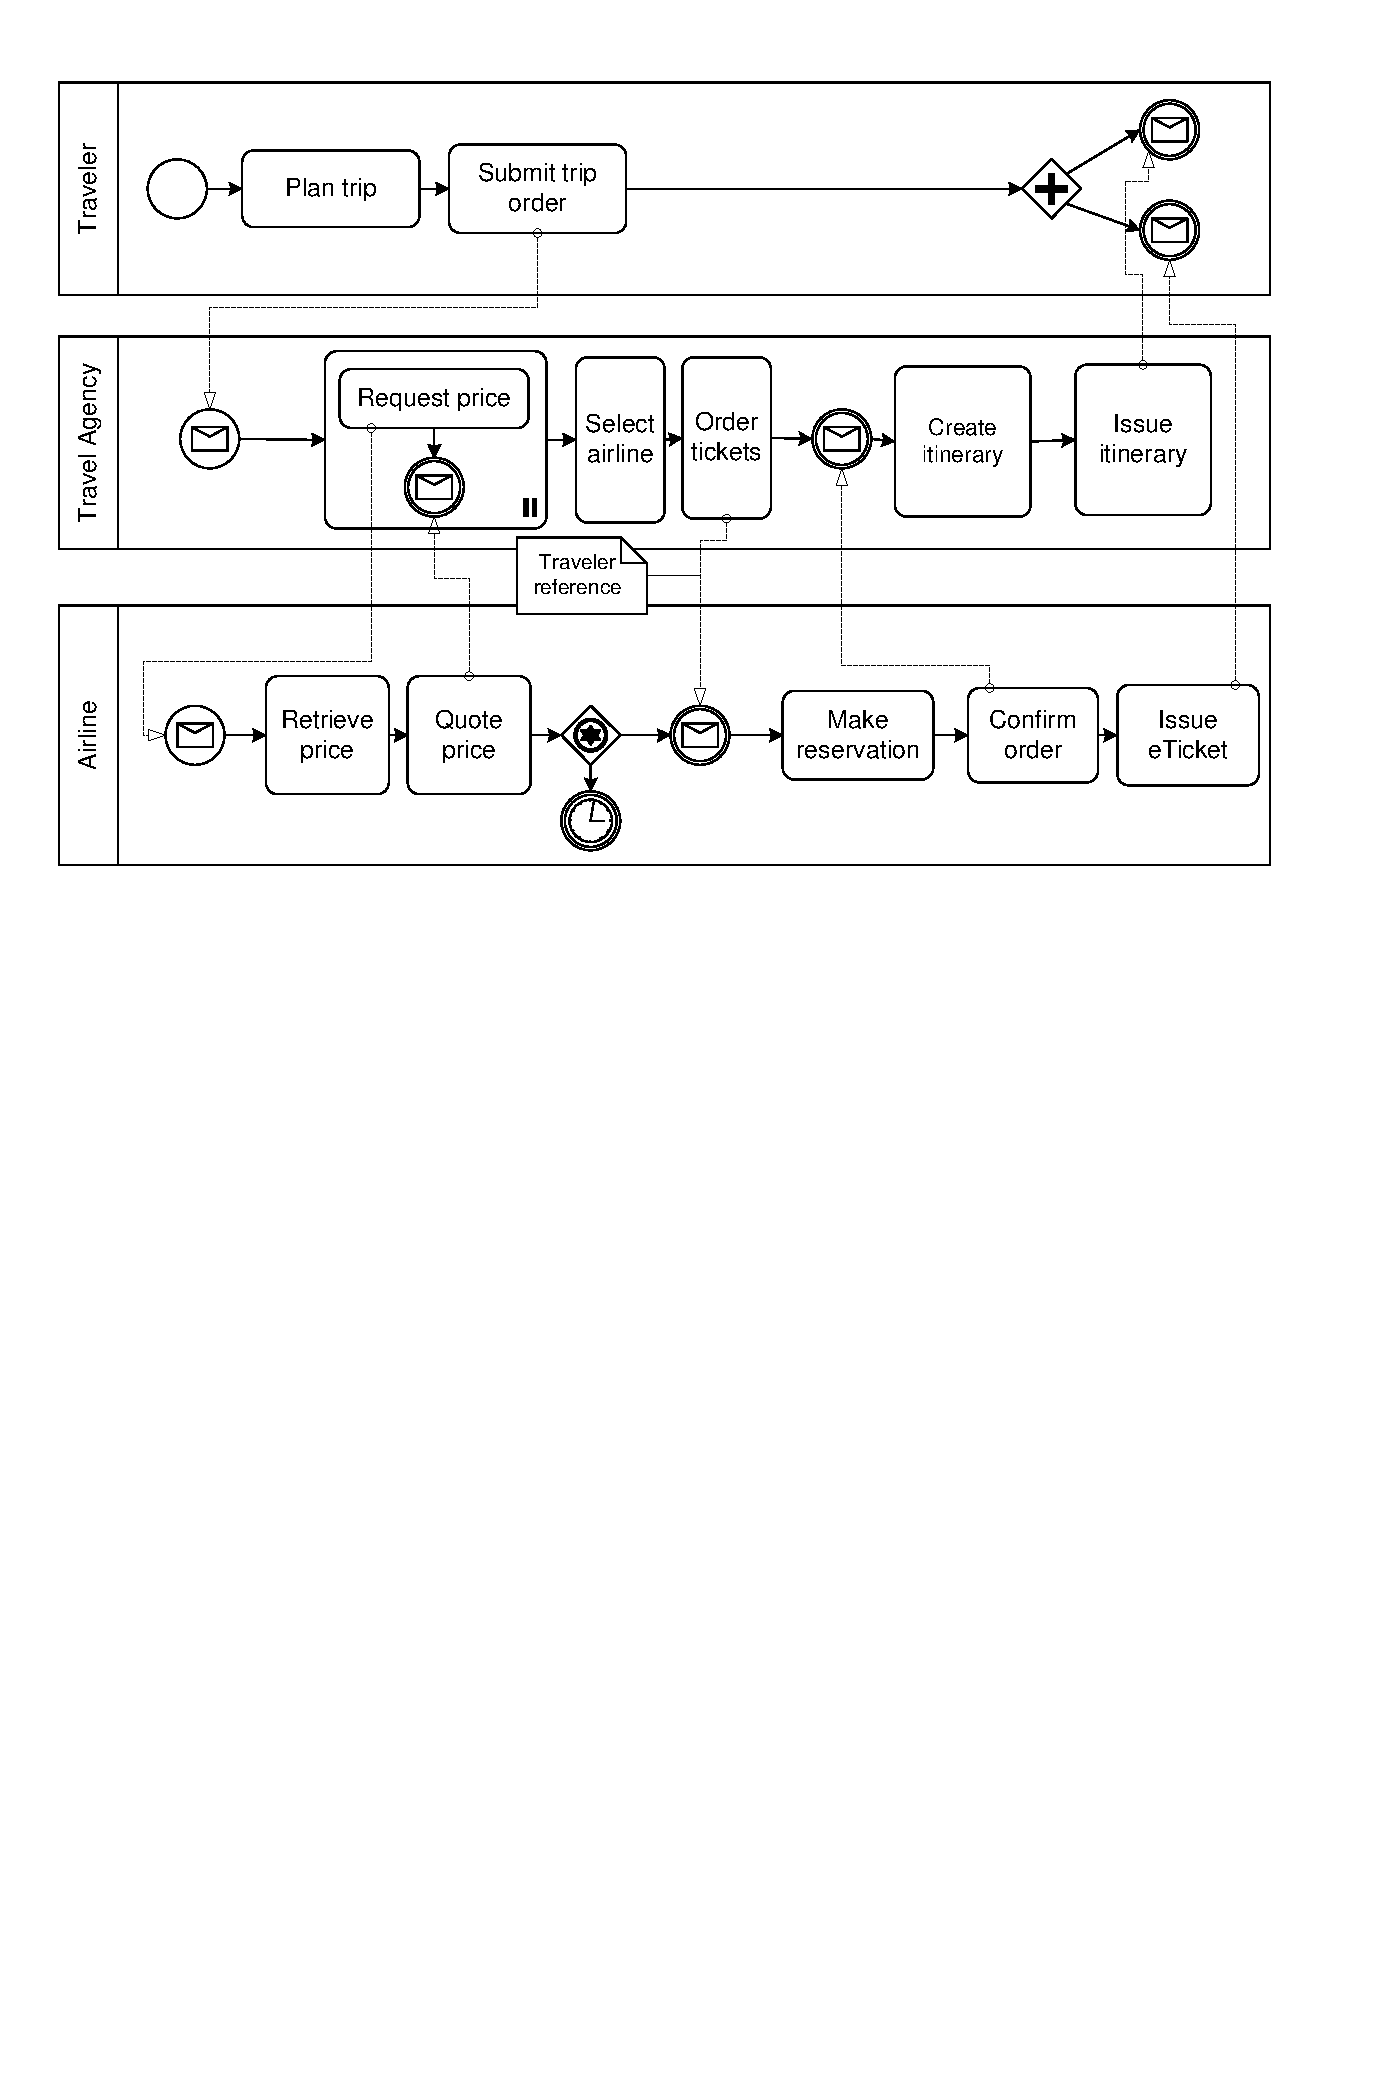
\includegraphics[width=\textwidth]{choreography.pdf}
    \caption{Choreography 2}
    \label{fig:subfigB}
  \end{subfigure}
  \hfill
  \begin{subfigure}{.3\textwidth}
    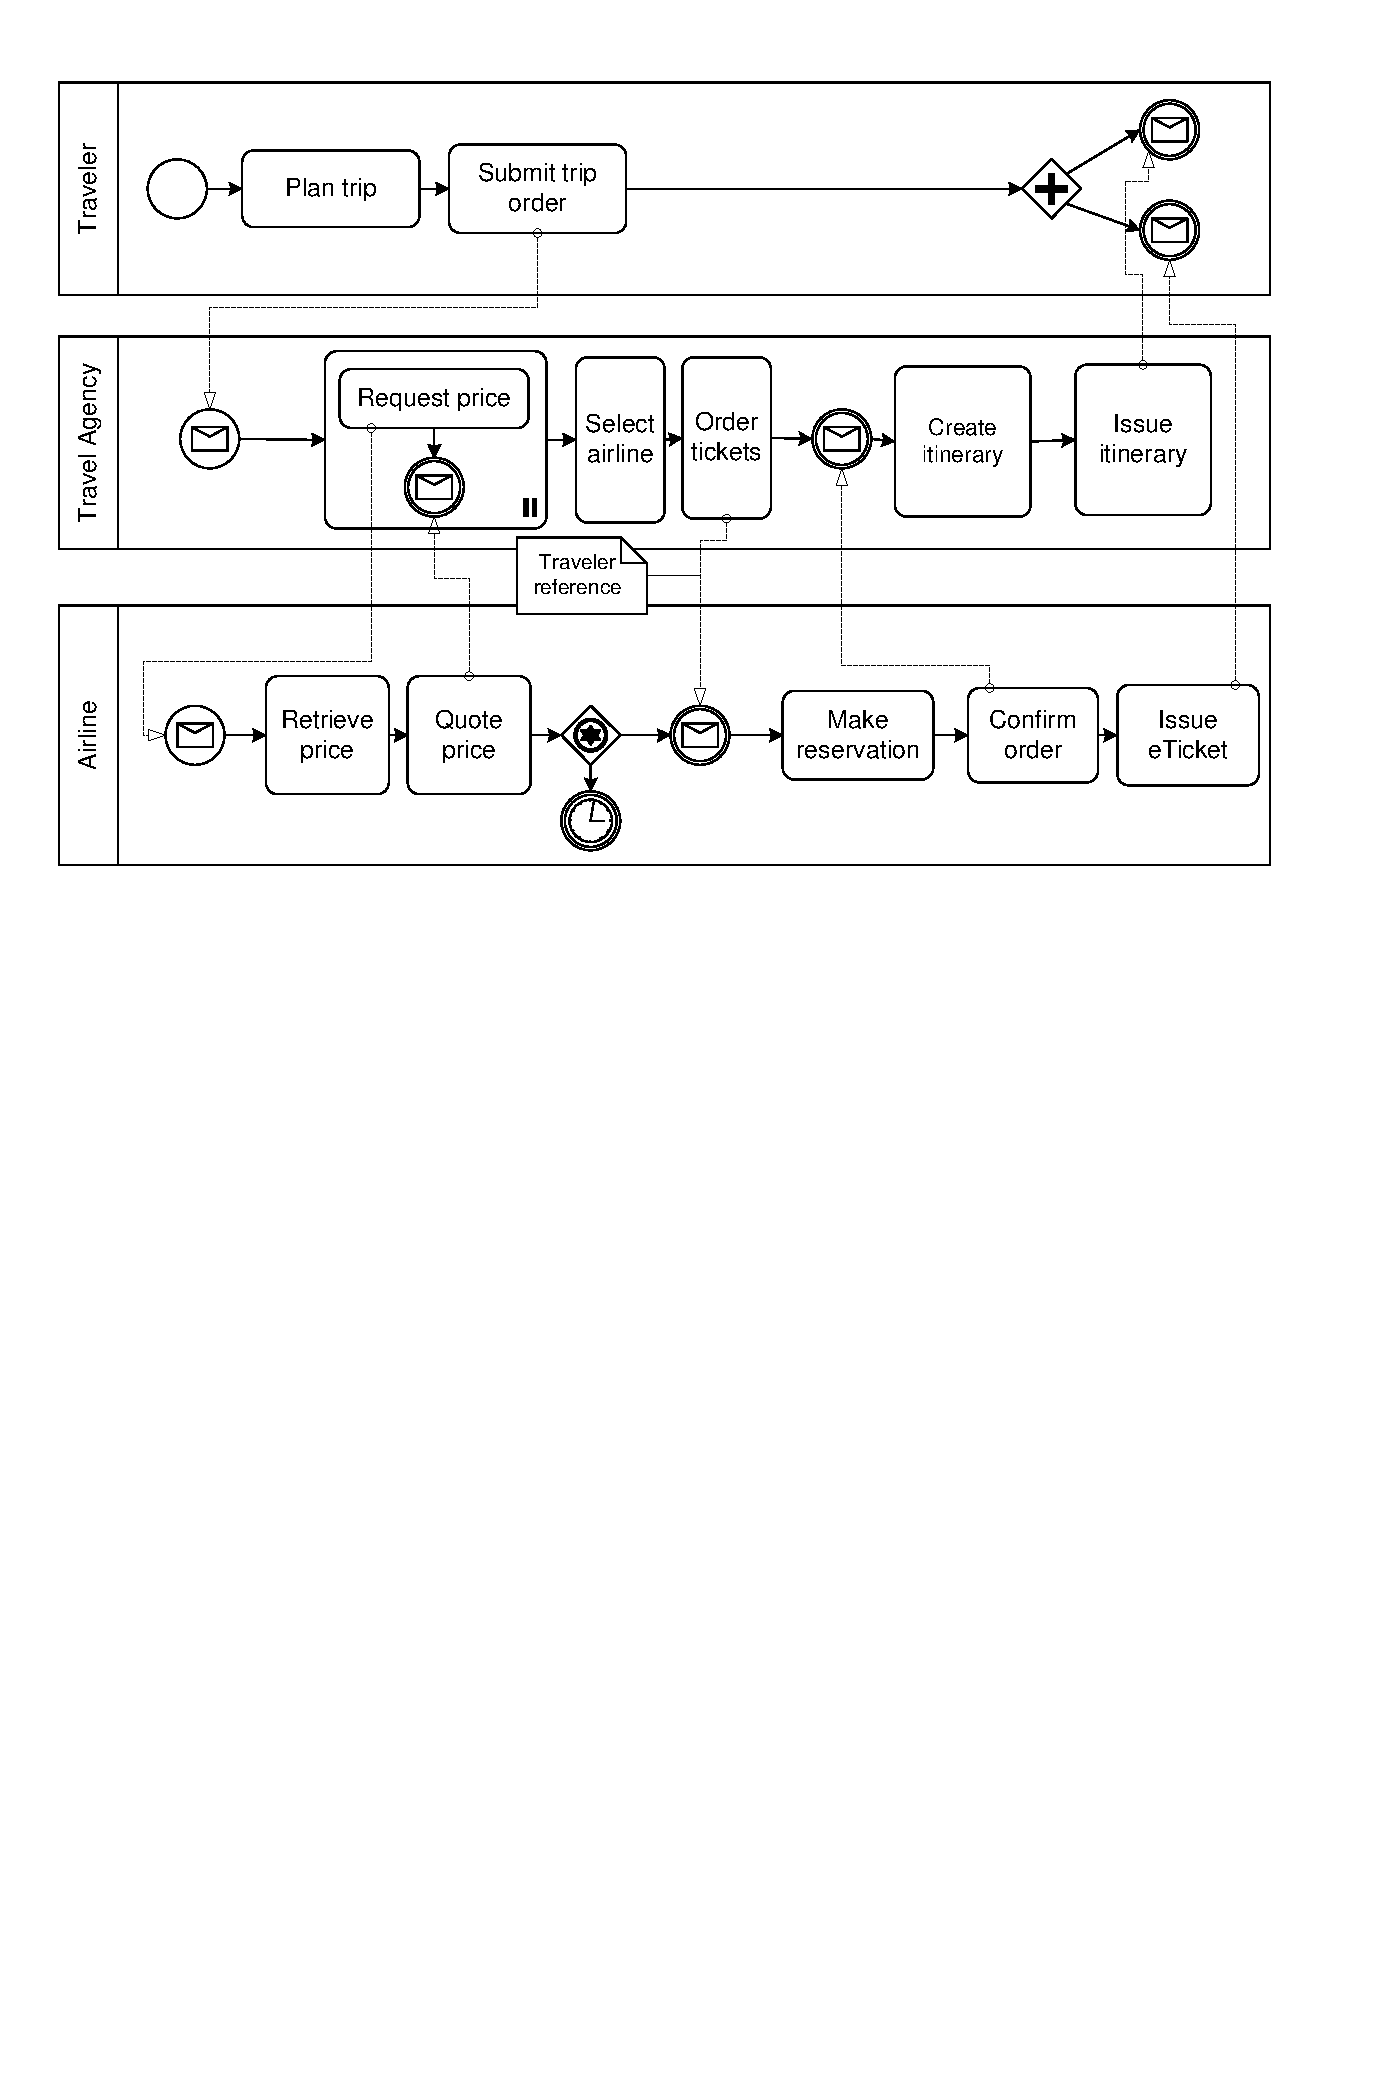
\includegraphics[width=.9\textwidth]{choreography.pdf}
    \caption{Choreography 3}
    \label{fig:subfigC}
  \end{subfigure}
  \caption{Example to place 3 illustrations next to each other. Further, it is possible to reference each separately.}
  \label{fig:subfig_example}
\end{figure}

\autoref{fig:subfig_example} shows the usage of the package subcaption.
It is indeed possible to reference to sub figures: \autoref{fig:subfigA}.

It is possible to convert SVGs to PDF directly during compilation.
This is described in the source code of latex-tipps.tex, but commented out.

\iffalse % <-- Take this away if inkscape is in the path
  The SVG in \autoref{fig:directSVG} is directly included, while the text in the SVG in \autoref{fig:latexSVG} is set using pdflatex.
  If you want to see the graphics, inkscape must be in PATH and in the text source \texttt{\textbackslash{}iffalse} and \text{\textbackslash{}iftrue} have to be commented out.

  \begin{figure}
    \centering
    
\includegraphics{svgexample.svg}
    \caption{SVG directly included}
    \label{fig:directSVG}
  \end{figure}

  \begin{figure}
    \centering
    \def\svgwidth{.4\textwidth}
    \includesvg{svgexample}
    \caption{Text in SVN set via \LaTeX{}}
    \label{fig:latexSVG}
  \end{figure}
\fi % <-- Take this away if inkscape is in the path



\section{More Illustrations}
\autoref{fig:AnhangsChor,fig:AnhangsChor2} show two choreographies, which should further explain the facts. The second figure is rotated 90 degrees to demonstrate the \texttt{pdflscape} package.

\begin{figure}
  \centering
  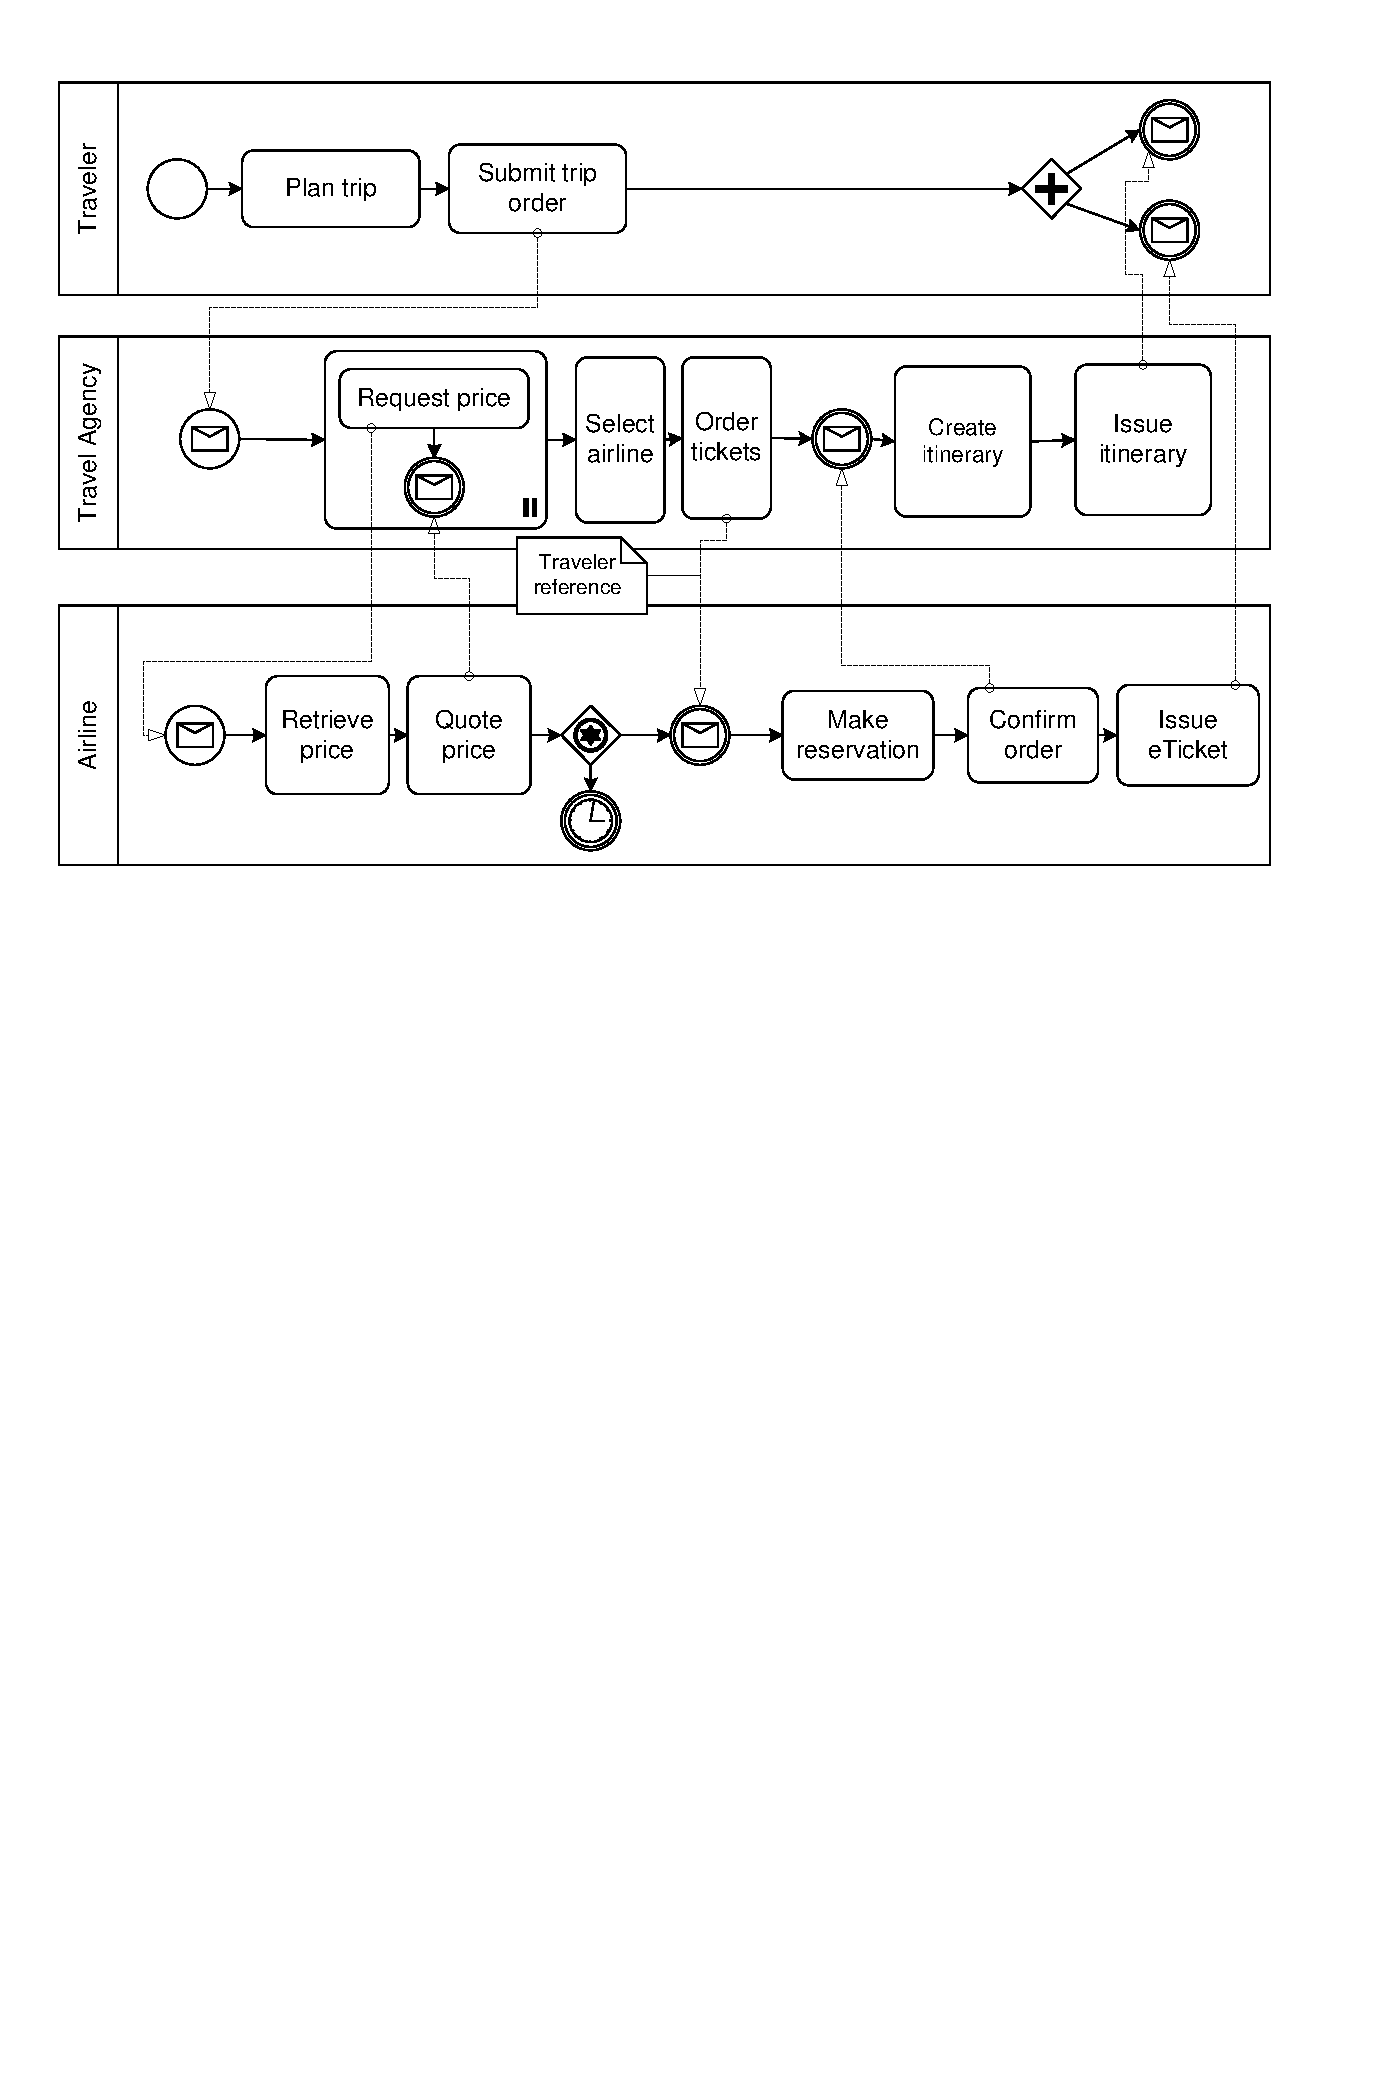
\includegraphics[width=\textwidth]{choreography.pdf}
  \caption{Example Choreography I}
  \label{fig:AnhangsChor}
\end{figure}

\begin{landscape}
  %sidewaysfigure
  \begin{figure}
    \centering
    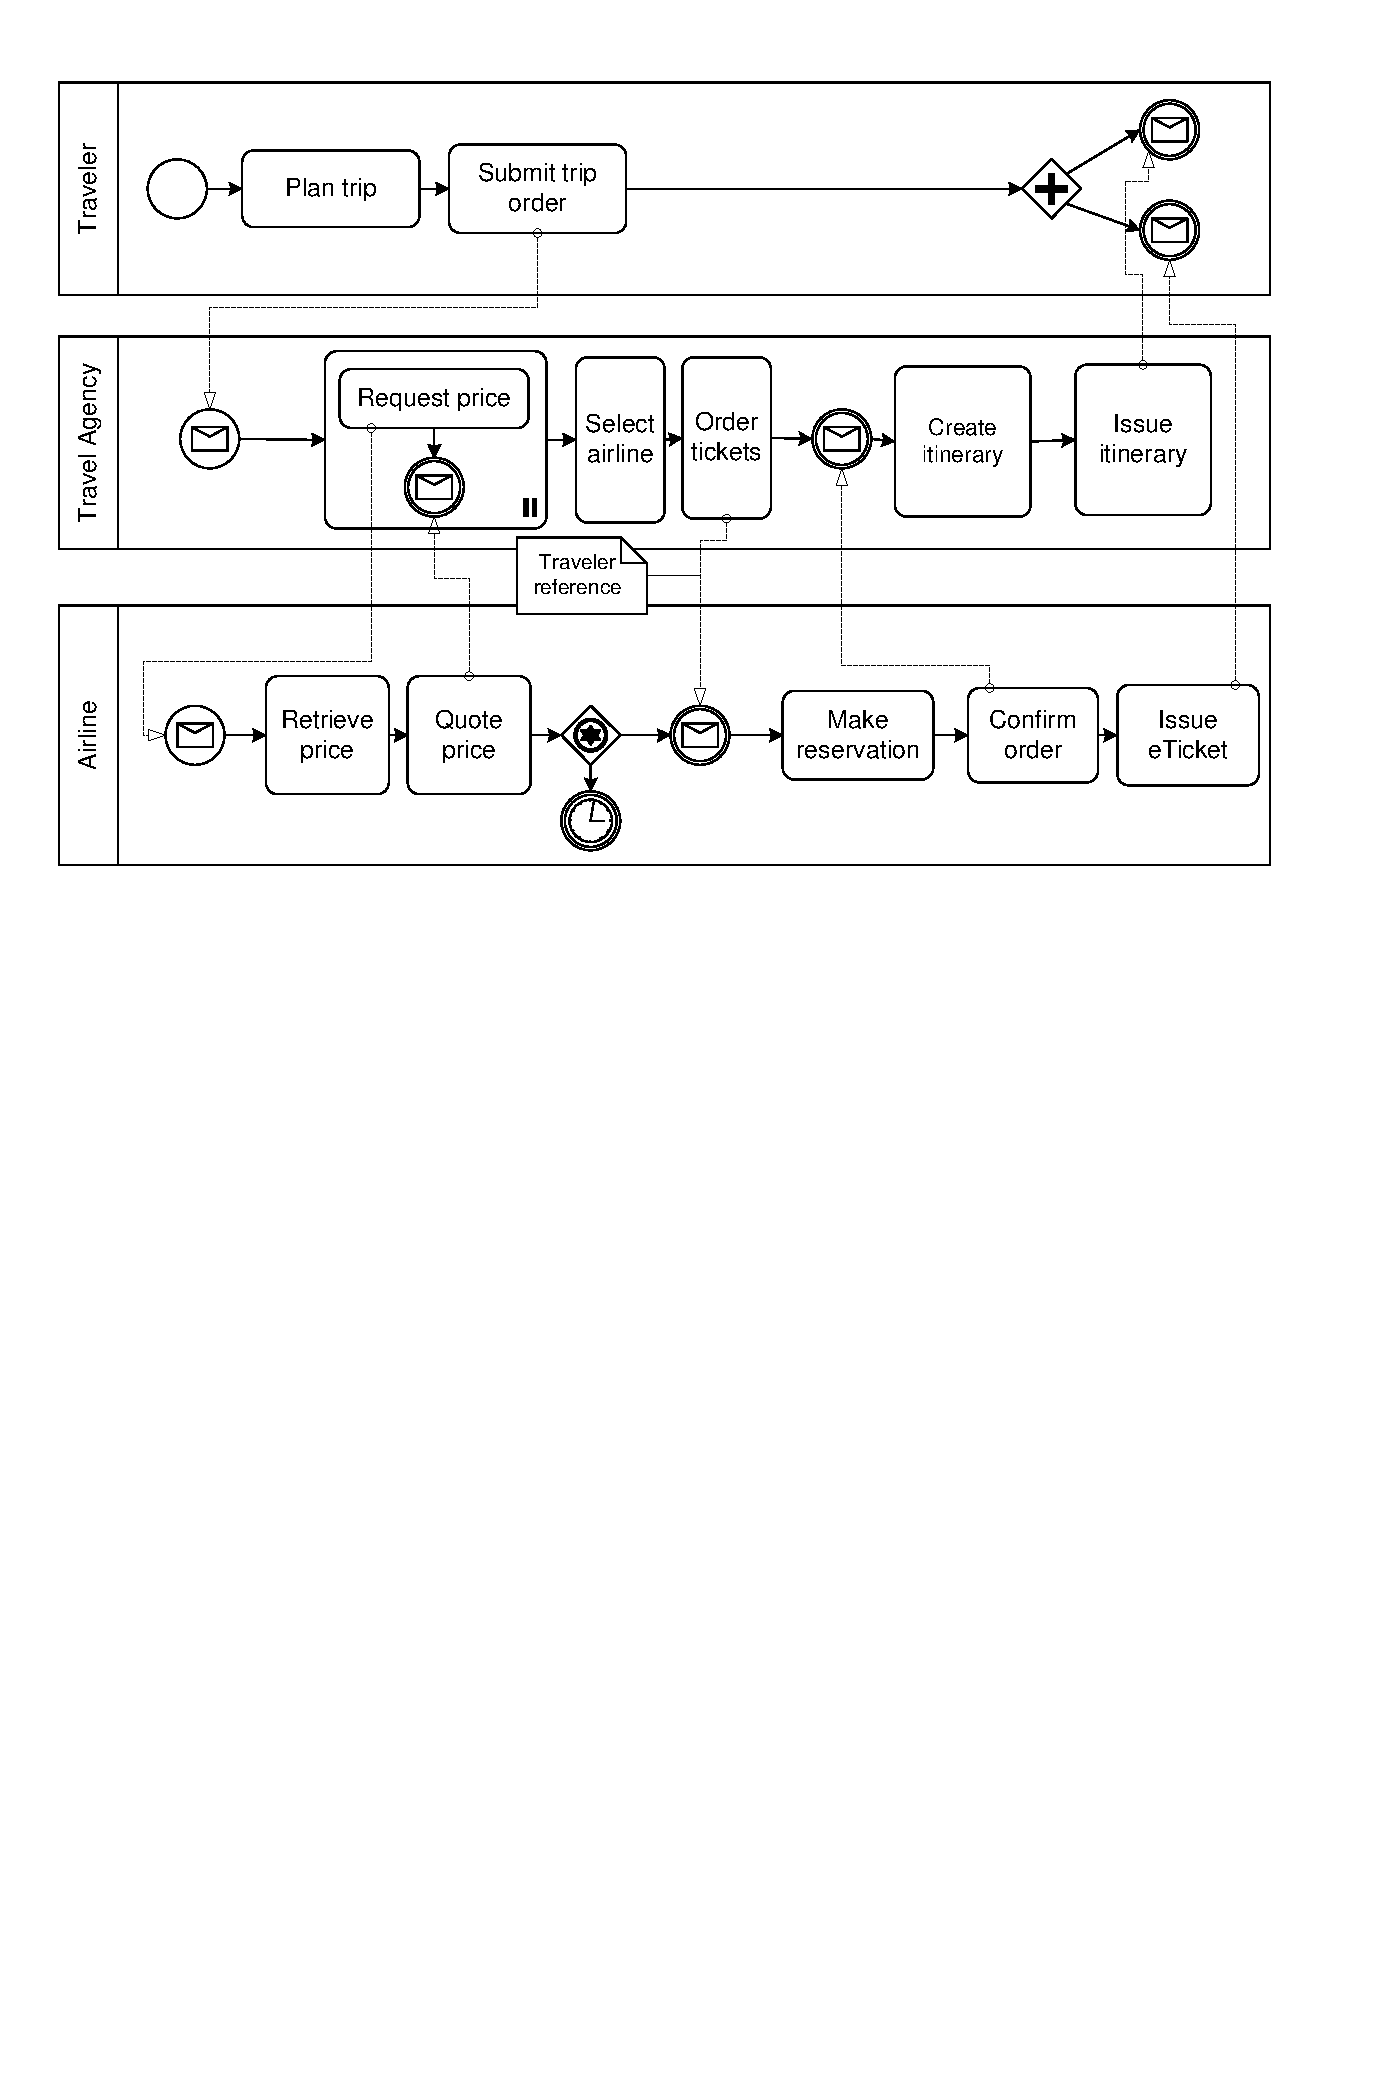
\includegraphics[width=\textwidth]{choreography.pdf}
    \caption{Example Choreography II}
    \label{fig:AnhangsChor2}
  \end{figure}
\end{landscape}


\IfFileExists{pgfplots.sty}{
  %%%%%%%%%%%%%%%%%%%%%%%%%%%%%%%%%%%%%%%%%%%%%%%%%%%%%%%%%%%%%%%%%%%%%%%%%%%%%%
  \section{Plots with pgfplots}
  %%%%%%%%%%%%%%%%%%%%%%%%%%%%%%%%%%%%%%%%%%%%%%%%%%%%%%%%%%%%%%%%%%%%%%%%%%%%%%
  The package pdfplots provides plotting of functions directly in \LaTeX~like with matlab or gnuplot. Some visual examples are available here\footnote{\url{http://texdoc.net/pkg/visualtikz}}.
  \begin{figure}[h]
    \centering
    \begin{tikzpicture}
      \begin{axis}[xlabel=$x$,
          ylabel=$\sin(x)$]
        \addplot {sin(deg(x))};  % Print sine function
      \end{axis}
    \end{tikzpicture}
    \caption{Plot of $\sin(x)$ direclty inside the figure environment with pgfplots.}
  \end{figure}

  \begin{figure}[h]
    \centering
    \begin{tikzpicture}
      \begin{axis}[xlabel=$x$,
          ylabel=$y$]
        \addplot table [x=a, y=c, col sep=comma] {data/data.csv};  % Read coordinates from csv file and plot them
      \end{axis}
    \end{tikzpicture}
    \caption{Coordinates $x$ and $y$ read from csv file and plotted pgfplots.}
  \end{figure}

}{}


%%%%%%%%%%%%%%%%%%%%%%%%%%%%%%%%%%%%%%%%%%%%%%%%%%%%%%%%%%%%%%%%%%%%%%%%%%%%%%
\section{Figures with tikz}
%%%%%%%%%%%%%%%%%%%%%%%%%%%%%%%%%%%%%%%%%%%%%%%%%%%%%%%%%%%%%%%%%%%%%%%%%%%%%%
The tikz is a package for creating graphics programmatically. With this package grids or other regular strucutres can be easliy generated.

\begin{figure}[ht]
  \centering
  \begin{tikzpicture}
    \draw(0,0) rectangle (4,4);
    \foreach \x in {0.5,1,1.5,2,2.5,3,3.5}
    \foreach \y in {0.5,1,1.5,2,2.5,3,3.5}
    \draw(\x,\y) circle (1pt);
  \end{tikzpicture}
  \caption{A regular grid genrated with easily with two for loops.}\label{fig:tikz_example}
\end{figure}


%%%%%%%%%%%%%%%%%%%%%%%%%%%%%%%%%%%%%%%%%%%%%%%%%%%%%%%%%%%%%%%%%%%%%%%%%%%%%%
\section{UML diagrams using tikz-uml}
%%%%%%%%%%%%%%%%%%%%%%%%%%%%%%%%%%%%%%%%%%%%%%%%%%%%%%%%%%%%%%%%%%%%%%%%%%%%%%

\autoref{fig:uml} presents a class diagram typeset using tikz-uml.

\begin{figure}
  \centering
  \begin{tikzpicture}
  \begin{umlpackage}{p}
  \begin{umlpackage}{sp1}
  \umlclass[template=T]{A}{
    n : uint \\ t : float
  }{}
  \umlclass[y=-3]{B}{
    d : double
  }{
    \umlvirt{setB(b : B) : void} \\ getB() : B}
  \end{umlpackage}
  \begin{umlpackage}[x=10,y=-6]{sp2}
  \umlinterface{C}{
    n : uint \\ s : string
  }{}
  \end{umlpackage}
  \umlclass[x=2,y=-10]{D}{
    n : uint
    }{}
  \end{umlpackage}

  \umlassoc[geometry=-|-, arg1=tata, mult1=*, pos1=0.3, arg2=toto, mult2=1, pos2=2.9, align2=left]{C}{B}
  \umlunicompo[geometry=-|, arg=titi, mult=*, pos=1.7, stereo=vector]{D}{C}
  \umlimport[geometry=|-, anchors=90 and 50, name=import]{sp2}{sp1}
  \umlaggreg[arg=tutu, mult=1, pos=0.8, angle1=30, angle2=60, loopsize=2cm]{D}{D}
  \umlinherit[geometry=-|]{D}{B}
  \umlnote[x=2.5,y=-6, width=3cm]{B}{A note with respect to class B}
  \umlnote[x=7.5,y=-2]{import-2}{A anotation}
  \end{tikzpicture}
  \caption{Class diagram generated with tikz-uml. Example adapted from Nicolas Kielbasiewicz.}
  \label{fig:uml}
\end{figure}

\section{UML diagrams using PlantUML}

In case \lualatex{} is used and PlantUML is installed, UML diagrams can be defined using PlantUML.

% Only works if "--shell-escape" is activated. Please activate only if you are sure, your compilation settings are correct
%\IfFileExists{plantuml.sty}{\input{latexhints-english-plantuml}}{}


%%%%%%%%%%%%%%%%%%%%%%%%%%%%%%%%%%%%%%%%%%%%%%%%%%%%%%%%%%%%%%%%%%%%%%%%%%%%%%
\section{Linguistic Forests}
%%%%%%%%%%%%%%%%%%%%%%%%%%%%%%%%%%%%%%%%%%%%%%%%%%%%%%%%%%%%%%%%%%%%%%%%%%%%%%

\begin{filecontents*}{\democodefile}
\begin{forest}
  [VP
    [DP]
    [V’
      [V]
      [DP]
    ]
  ]
\end{forest}
\end{filecontents*}
\PrintDemo{style=parallel}


%%%%%%%%%%%%%%%%%%%%%%%%%%%%%%%%%%%%%%%%%%%%%%%%%%%%%%%%%%%%%%%%%%%%%%%%%%%%%%
\section{Tables}
%%%%%%%%%%%%%%%%%%%%%%%%%%%%%%%%%%%%%%%%%%%%%%%%%%%%%%%%%%%%%%%%%%%%%%%%%%%%%%
\autoref{tab:Ergebnisse} shows results and \autoref{tab:Werte} shows how numerical data can be represented in a table.
\begin{table}
  \centering
  \begin{tabular}{ccc}
    \toprule
    \multicolumn{2}{c}{\textbf{summed}} & \textbf{Title}                                                          \\ \midrule
    Table                                      & as                                                           & in      \\
    \url{tabsatz.pdf}                            & recommended                                                     & gesetzt \\

    \multirow{2}{*}{Example}                    & \multicolumn{2}{c}{a nice example}                                \\
                                                 & \multicolumn{2}{c}{for using \qq{multirow}}           \\
    \bottomrule
  \end{tabular}
  \caption[Example Table]{Exampe Table -- see \url{http://www.ctan.org/tex-archive/info/german/tabsatz/}}
  \label{tab:Ergebnisse}
\end{table}

\begin{table}
  \centering
  \begin{tabular}{l *{8}{d{3.2}}}
    \toprule

                         & \multicolumn{2}{c}{\textbf{Parameter 1}} & \multicolumn{2}{c}{\textbf{Parameter 2}} & \multicolumn{2}{c}{\textbf{Parameter 3}} & \multicolumn{2}{c}{\textbf{Parameter 4}}                                                                                                                                       \\
    \cmidrule(r){2-3}\cmidrule(lr){4-5}\cmidrule(lr){6-7}\cmidrule(l){8-9}

    \textbf{Bedingungen} & \multicolumn{1}{c}{\textbf{M}}           & \multicolumn{1}{c}{\textbf{SD}}          & \multicolumn{1}{c}{\textbf{M}}           & \multicolumn{1}{c}{\textbf{SD}}          & \multicolumn{1}{c}{\textbf{M}} & \multicolumn{1}{c}{\textbf{SD}} & \multicolumn{1}{c}{\textbf{M}} & \multicolumn{1}{c}{\textbf{SD}} \\
    \midrule

    W                    & 1.1                                      & 5.55                                     & 6.66                                     & .01                                      &                                &                                 &                                &                                 \\
    X                    & 22.22                                    & 0.0                                      & 77.5                                     & .1                                       &                                &                                 &                                &                                 \\
    Y                    & 333.3                                    & .1                                       & 11.11                                    & .05                                      &                                &                                 &                                &                                 \\
    Z                    & 4444.44                                  & 77.77                                    & 14.06                                    & .3                                       &                                &                                 &                                &                                 \\
    \bottomrule
  \end{tabular}

  \caption{Example table for 4 constraints (W-Z), each having 4 parameters with (M und SD). Note: use always the same number of decimal places.}
  \label{tab:Werte}
\end{table}

\IfFileExists{pgfplotstable.sty}{

\subsection{Tables with pgfplots}
With the pgfplotstable package tables can be directly generated from a csv file.

\begin{table}[h]
\centering
\pgfplotstabletypeset[
col sep = comma,
every head row/.style={before row=\toprule,after row=\midrule},
every last row/.style={after row=\bottomrule},
display columns/0/.style={string type,column name={}}
]
{data/data.csv}
\caption{Table direclty generated from the values of a csf file.}
\end{table}
}{}


\section{Tables spanning multiple pages}


\begin{longtable}{|l|l|l|}
\caption{A sample long table.} \label{tab:long} \\

\hline \multicolumn{1}{|c|}{\textbf{First column}} & \multicolumn{1}{c|}{\textbf{Second column}} & \multicolumn{1}{c|}{\textbf{Third column}} \\ \hline
\endfirsthead

\multicolumn{3}{c}%
{{\bfseries \tablename\ \thetable{} -- continued from previous page}} \\
\hline \multicolumn{1}{|c|}{\textbf{First column}} & \multicolumn{1}{c|}{\textbf{Second column}} & \multicolumn{1}{c|}{\textbf{Third column}} \\ \hline
\endhead

\hline \multicolumn{3}{|r|}{{Continued on next page}} \\ \hline
\endfoot

\hline \hline
\endlastfoot

A & BC & D \\
A & BC & D \\
A & BC & D \\
A & BC & D \\
A & BC & D \\
A & BC & D \\
A & BC & D \\
A & BC & D \\
A & BC & D \\
A & BC & D \\
A & BC & D \\
A & BC & D \\
A & BC & D \\
A & BC & D \\
A & BC & D \\
A & BC & D \\
A & BC & D \\
A & BC & D \\
A & BC & D \\
A & BC & D \\
A & BC & D \\
A & BC & D \\
A & BC & D \\
A & BC & D \\
A & BC & D \\
A & BC & D \\
A & BC & D \\
A & BC & D \\
A & BC & D \\
A & BC & D \\
A & BC & D \\
A & BC & D \\
A & BC & D \\
A & BC & D \\
A & BC & D \\
A & BC & D \\
A & BC & D \\
A & BC & D \\
A & BC & D \\
A & BC & D \\
A & BC & D \\
A & BC & D \\
A & BC & D \\
A & BC & D \\
A & BC & D \\
A & BC & D \\
A & BC & D \\
A & BC & D \\
A & BC & D \\
A & BC & D \\
A & BC & D \\
A & BC & D \\
A & BC & D \\
A & BC & D \\
A & BC & D \\
A & BC & D \\
A & BC & D \\
A & BC & D \\
A & BC & D \\
A & BC & D \\
A & BC & D \\
A & BC & D \\
A & BC & D \\
A & BC & D \\
A & BC & D \\
A & BC & D \\
A & BC & D \\
A & BC & D \\
A & BC & D \\
A & BC & D \\
A & BC & D \\
A & BC & D \\
A & BC & D \\
A & BC & D \\
A & BC & D \\
A & BC & D \\
A & BC & D \\
A & BC & D \\
A & BC & D \\
A & BC & D \\
\end{longtable}


%%%%%%%%%%%%%%%%%%%%%%%%%%%%%%%%%%%%%%%%%%%%%%%%%%%%%%%%%%%%%%%%%%%%%%%%%%%%%%
\section{Abbreviations}
%%%%%%%%%%%%%%%%%%%%%%%%%%%%%%%%%%%%%%%%%%%%%%%%%%%%%%%%%%%%%%%%%%%%%%%%%%%%%%
At the first pass the \gls{fr} was 5.
At the second pass was \gls{fr} 3.
The plural form can be seen here: \glspl{er}.
To demonstrate what the list of abbreviations looks like for longer description texts, \glspl{rdbms} must be mentioned here.

With \verb+\gls{...}+ you can enter abbreviations, the first time you call it, the long form is used.
When reusing \verb+\gls{..}+ the short form is automatically displayed.
The abbreviation is also automatically inserted in the abbreviation list.
With \verb+\glspl{...}+ the plural form is used.
If you want the short form to appear directly at the first use, you can use \verb+\glsunset{..}+ to mark an abbreviation as already used.
The opposite is achieved with \verb+\glsreset{..}+.

Abbreviations are defined in \verb+\content\ausarbeitung.tex+ by means of \verb+\newacronym{...}{...}{...}+.

More information at: \url{http://tug.ctan.org/macros/latex/contrib/glossaries/glossariesbegin.pdf}
%%%%%%%%%%%%%%%%%%%%%%%%%%%%%%%%%%%%%%%%%%%%%%%%%%%%%%%%%%%%%%%%%%%%%%%%%%%%%%
\section{References}
%%%%%%%%%%%%%%%%%%%%%%%%%%%%%%%%%%%%%%%%%%%%%%%%%%%%%%%%%%%%%%%%%%%%%%%%%%%%%%
For distant sections \qq{varioref} is recommended:
\qq{See \vref{sec:mf}}.
The command \texttt{\textbackslash{}vref} works similar to \texttt{\textbackslash{}cref} the difference beeing that a reference to the page is additionally added.
\texttt{vref}: \qq{\vref{sec:firstsectioninlatexhints}}, \texttt{cref}: \qq{\autoref{sec:firstsectioninlatexhints}}, \texttt{ref}: \qq{\ref{sec:firstsectioninlatexhints}}.

If \qq{varioref} causes difficulties, then \qq{cref} can be used instead.
This also creates the word \qq{section} automatically: \autoref{sec:mf}.
This is also possible for illustrations etc.
In English please use \verb1\autoref{...}1 (with large \qq{C} at the beginning).

%With MiKTeX installation from 2012-01-16 no longer necessary.
%If a section becomes longer than one page and you want to refer to a specific place in the section with \texttt{\textbackslash{}vref}, then you should use \texttt{\textbackslash{}phantomsection} then using \texttt{vref} will also display the correct page number.

%%The link location will be placed on the line below.
%%Tipp von http://en.wikibooks.org/wiki/LaTeX/Labels_and_Cross-referencing#The_hyperref_package_and_.5Cphantomsection
%\phantomsection
%\label{alabel}
%View the example for \texttt{\textbackslash{}phantomsection} in the \LaTeX{} source code.

%Here is the example: See Section \vref{hack1} and Section \vref{hack2}.
%%%%%%%%%%%%%%%%%%%%%%%%%%%%%%%%%%%%%%%%%%%%%%%%%%%%%%%%%%%%%%%%%%%%%%%%%%%%%%
\section{Definitions}
%%%%%%%%%%%%%%%%%%%%%%%%%%%%%%%%%%%%%%%%%%%%%%%%%%%%%%%%%%%%%%%%%%%%%%%%%%%%%%
\begin{definition}[Title]
  \label{def:def1}
  Definition Text
\end{definition}

\autoref{def:def1} shows \ldots

%%%%%%%%%%%%%%%%%%%%%%%%%%%%%%%%%%%%%%%%%%%%%%%%%%%%%%%%%%%%%%%%%%%%%%%%%%%%%%
\section{Footnotes}
%%%%%%%%%%%%%%%%%%%%%%%%%%%%%%%%%%%%%%%%%%%%%%%%%%%%%%%%%%%%%%%%%%%%%%%%%%%%%%
Footnotes are provided by the command \verb+\footnote{...}+\footnote{\label{fussnote}Example footnote.}. Citing footnotes is possible by provinding a label\verb+\footnote{\label{...}...}+ and cite the footnote with \verb+\autoref{...}+ in the text\autoref{fussnote}.
%%%%%%%%%%%%%%%%%%%%%%%%%%%%%%%%%%%%%%%%%%%%%%%%%%%%%%%%%%%%%%%%%%%%%%%%%%%%%%

%%%%%%%%%%%%%%%%%%%%%%%%%%%%%%%%%%%%%%%%%%%%%%%%%%%%%%%%%%%%%%%%%%%%%%%%%%%%%%
\section{Various Things}
%%%%%%%%%%%%%%%%%%%%%%%%%%%%%%%%%%%%%%%%%%%%%%%%%%%%%%%%%%%%%%%%%%%%%%%%%%%%%%
\label{sec:diff}
\ifdeutsch
  Numbers (123\,654\,789) are nicely set.
  Either in a line or as non-lining figure.
  The latter is reached by parameter \texttt{osf} at package \texttt{libertine} or.\ \texttt{mathpazo} in \text{fonts.tex}.
\fi

\begin{filecontents*}{\democodefile}
\begin{compactenum}[I.]
  \item You can also keep the numbering compact thanks to paralist
  \item and switch to a different numbering
\end{compactenum}
\end{filecontents*}
\PrintDemo{style=parallel}

The words \qq{workflow} and \qq{dwarflike} can be copied from the PDF and pasted to a text file.

\begin{filecontents*}{\democodefile}
In case \LuaLaTeX{} is used as compiler, there is no ligature at \qq{f\/l} in the word \qq{dwarflike} (in contrast to \qq{fl} at \qq{workflow}).
In other words: \qq{dwarflike} and \qq{dwarf\/like} look the same in the PDF.
In case they do not, there is an issue with Lua\LaTeX{} and the selnolig package.
\end{filecontents*}
\PrintDemo{style=parallel}
% Meta comment: The precise form of the optimal ligation suppression command may vary depending on the character pairs involved - see https://tex.stackexchange.com/q/28437/9075


%%%%%%%%%%%%%%%%%%%%%%%%%%%%%%%%%%%%%%%%%%%%%%%%%%%%%%%%%%%%%%%%%%%%%%%%%%%%%%
\section{Closing remarks}
%%%%%%%%%%%%%%%%%%%%%%%%%%%%%%%%%%%%%%%%%%%%%%%%%%%%%%%%%%%%%%%%%%%%%%%%%%%%%%
Please feel free to provide enhancements for this template and create a new ticket on GitHub (\url{https://github.com/latextemplates/uni-stuttgart-computer-science-template/issues}).


\pagestyle{empty}
\renewcommand*{\chapterpagestyle}{empty}
\Affirmation
\end{document}
